\section{Results from First Science Run}
\par
In this section, limits are placed on the elastic EFT operator couplings using data from the first science run (SR1) of LZ.
The region of interest considered here is limited to $\backsim$40 keV, i.e. 80 phd, rather than an extended energy window used in the previous section.
A more complete analysis using an extended recoil energy range is currently under preparation.
An analysis for SI and SD dark matter interactions have already been performed in this recoil energy range, with null results \cite{lz_ws_sr1_ref}.
As the analysis in this section uses the same dataset and cuts, only a limited summary of SR1 is presented here.
An overview of the calibration sources used for SR1 is described in \autoref{sec:lz_calibrations}.
A more complete description of the backgrounds in SR1 is laid out in \cite{lz_sr1_backgrounds_ref}.

\subsection{Overview of SR1}
\par
SR1 ran for a total of 116 days from 23 December 2021 to 18 April 2022 during which time the detector was in a stable running state.
As was mentioned in \autoref{sec:od_analysis_backgrounds}, several interruptions occurred for both calibration runs and system maintenance reducing the data set down to 89 live-days.
The length of time running was driven by a requirement to demonstrate physics capability and so only ran until the sensitivity to SI interactions was comparable to previous experiments.
SR1 was primarily an engineering run, and as such, no blinding or salting of the data set was performed.
As with any new detector, there are unexpected features that are best understood by being able to see and explore them.
In order to mitigate bias in analysis development, analysis cuts were developed in side bands and from calibration data.

\subsection{TPC Calibration}
\par
The spatial variation in $S1$ and $S2$ was corrected using primarily internal sources which are naturally dispersed throughout the detector volume.
${}^{83m}$Kr and ${}^{131m}$Xe were used for this along with injected tritium (injected as tritiated methane CH$_3$T).
Energy calibrations were performed with the internal sources as well as ${}^{129m}$Xe, which is monoenergetic at higher energies outside of the region considered here.
$g_1$ was determined to be 0.114$\pm$0.002 phd/photon and $g_2$ as 47.1$\pm$1.1 phd/electron \cite{lz_ws_sr1_ref}.
The size of a single electron light signal was measured as 57.6$\pm$1.9 phd/electron which gives an electron extraction efficiency of 80.5$\pm$3.7\% \cite{lz_ws_sr1_ref}.
For calibrating the detector model, NR events were produced using the DD neutrons and AmLi, whilst ER events were produced using tritium.
The detector response model was tuned to these measurements, which are shown in \autoref{fig:sr1_tpc_calibration} along with the ER and NR bands.
\begin{figure}
    \centering
    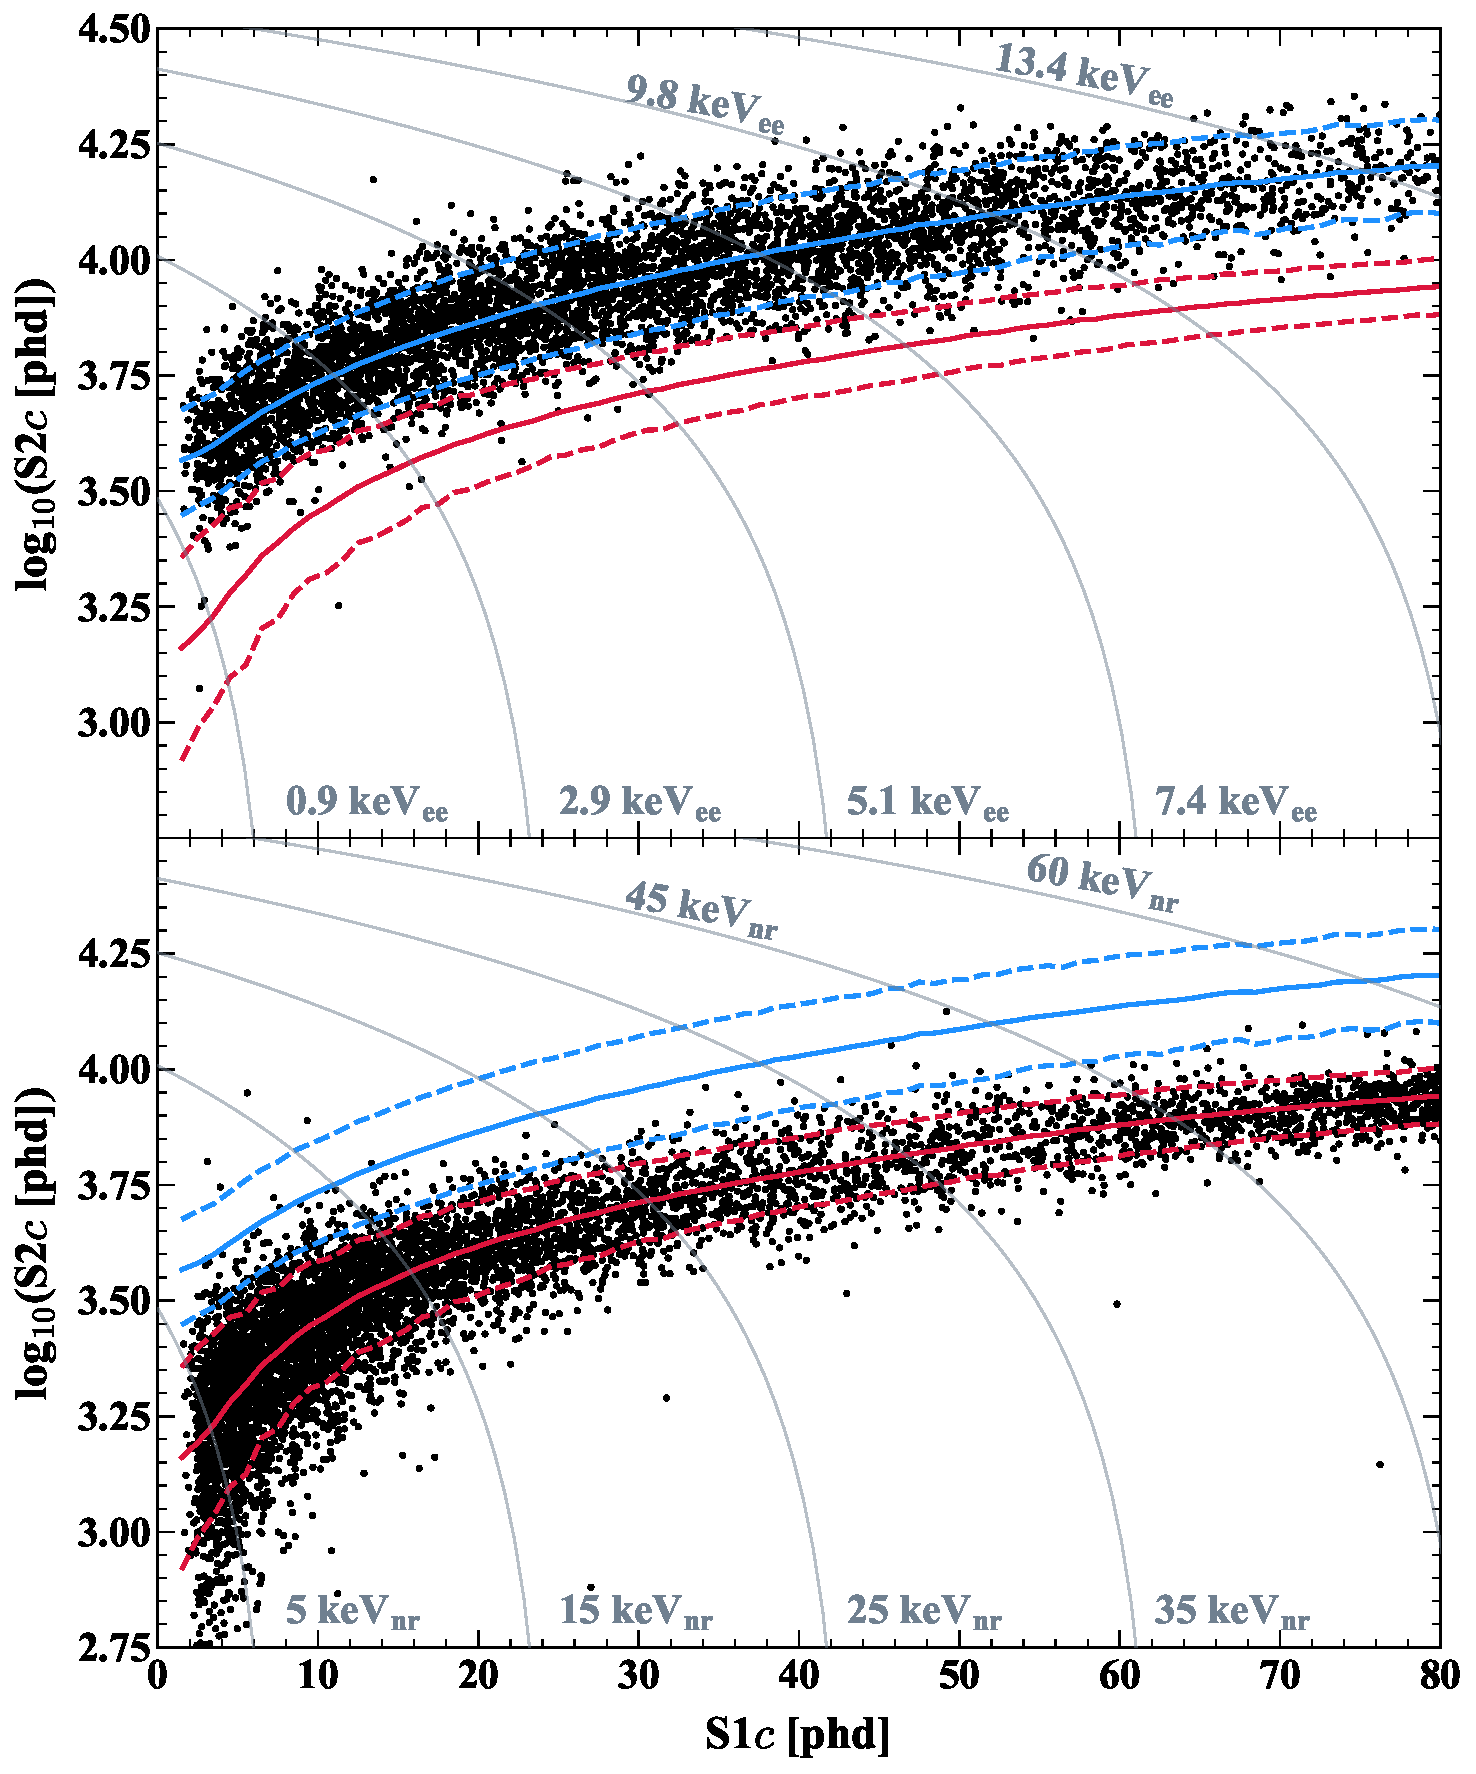
\includegraphics[width=10cm]{Figures/EFT/All_SR1_Plots/SR1WS_calOnly_0629_twoPanel.pdf}
    \caption{Calibration of ER and NR bands, shown in blue and red respectively.
             The solid line is the median, and the dashed are the 10\% and 90\% quantiles.
             \textbf{Top:} ER events produced by $\beta$-decays from injected CH$_3$T.
             \textbf{Bottom:} NR events produced by DD neutrons.
             }
    \label{fig:sr1_tpc_calibration}
\end{figure}

\subsection{Analysis Cuts}
\par
In addition to the core cuts that remove scatters that are inconsistent with dark matter that have been previously discussed, a multitude of other cuts were developed.
They fall broadly into three categories: live-time, S2-based cuts and S1-based cuts.
These three, along with the core cuts are briefly discussed below.


\subsubsection{Live-time cuts}
The live time cuts are named as such as they have a large adverse effect on the amount of data available.
Data is removed which shows uncharacteristic behaviour in the form of a high rate of pulses.
The two most significant cuts were an electron-train cut and a hot spot cut, together removing 35\% of the live-time.
After a large S2 event, a period of sustained high rate is observed. 
This is due to electrons attaching to impurities and then being released at some later time, causing a delayed extraction and an elevated rate after the S2.
Single photons are also observed after the same event, which is thought to be from delayed fluorescence.
The removal of time after an S2 until the detector rate settles corresponds to 29.8\% of live day loss.
Occasionally hot spots appeared in the TPC due to electron emission from the grids. 
These periods of time lasted approximately an hour at a time and reduced the live time by 6.6\%.
There were several other cuts in this category which combined reduced live-time by a further 1\%.

\subsubsection{S2 cuts}
This selection is designed to remove events which originate in or near the GXe. 
If the scatter occurs very close to the GXe then the time separation between the S1 and S2 is sufficiently low that the pulse finding algorithm cannot separate them. 
Similarly, GXe scatters would have merged S1 and S2s. 
Events with a poor position reconstruction (which uses the S2 hit pattern) are also removed this way.

\subsubsection{S1 cuts}
The S1 cuts were to ensure that the S1 pulse is not caused by a PMT process or a background process which would not produce an S2.
The most significant cut in this suite removed S1 events where a single PMT contributed significantly more to the waveform than neighbouring PMTs.

\subsubsection{Core cuts}
The core cuts focus on removing clean scatters in the TPC, but which do not match the properties of dark matter.
Only events with a single S1-S2 pulse pair are selected, and multiple S1 or multiple S2 events are removed.
\par
The fiducial region was defined in $z$ by the drift time (time between the S1 and S2 pulses) in the interval [86,936.5] $\mu$s, which corresponds to approximately 12.8 cm below the gate grid and 2.2 cm from the cathode grid.
$r$ was defined as either [4.0,5.0,5.2] cm from the TPC wall. 
The variation in $r$ is to remove regions where the electric field is non-uniform and effects from being close to the wall.
Within this region, the volume of xenon is 5.5$\pm$0.2 tonnes.
%\autoref{fig:sr1_fiducial_cut} shows the fiducial volume definition.
\par
The region of interest was defined as 3 phd $<$ S1$_c <$ 80 phd, S2 $>$ 600 phd and S2$_c <$ 10$^5$ phd.
The relation between S1$_c$ and recoil energy for nuclear recoil events is shown in \autoref{fig:sr1_detector_model_response_for_flat_nr}.
\par
The OD veto window was set to the value discussed in \autoref{sec:od_analysis_veto_efficiency} of 1200 $\mu$s, with an energy threshold of 200 keV.
The Skin veto window was set to 400 $\mu$s.
Additionally, a prompt veto window was implemented to remove events where the S1 is within [-300,300] ns of a pulse in either the Skin or OD to remove $\gamma$ events.

\par
The combined efficiency of all of these cuts is shown in \autoref{fig:sr1_nr_efficiency}.
A total of 335 events remained after the application of all of these cuts \cite{lz_ws_sr1_ref}.
%which are shown in \autoref{fig:henr_ws_sr1_events}.

%\begin{figure}
%    \centering
%    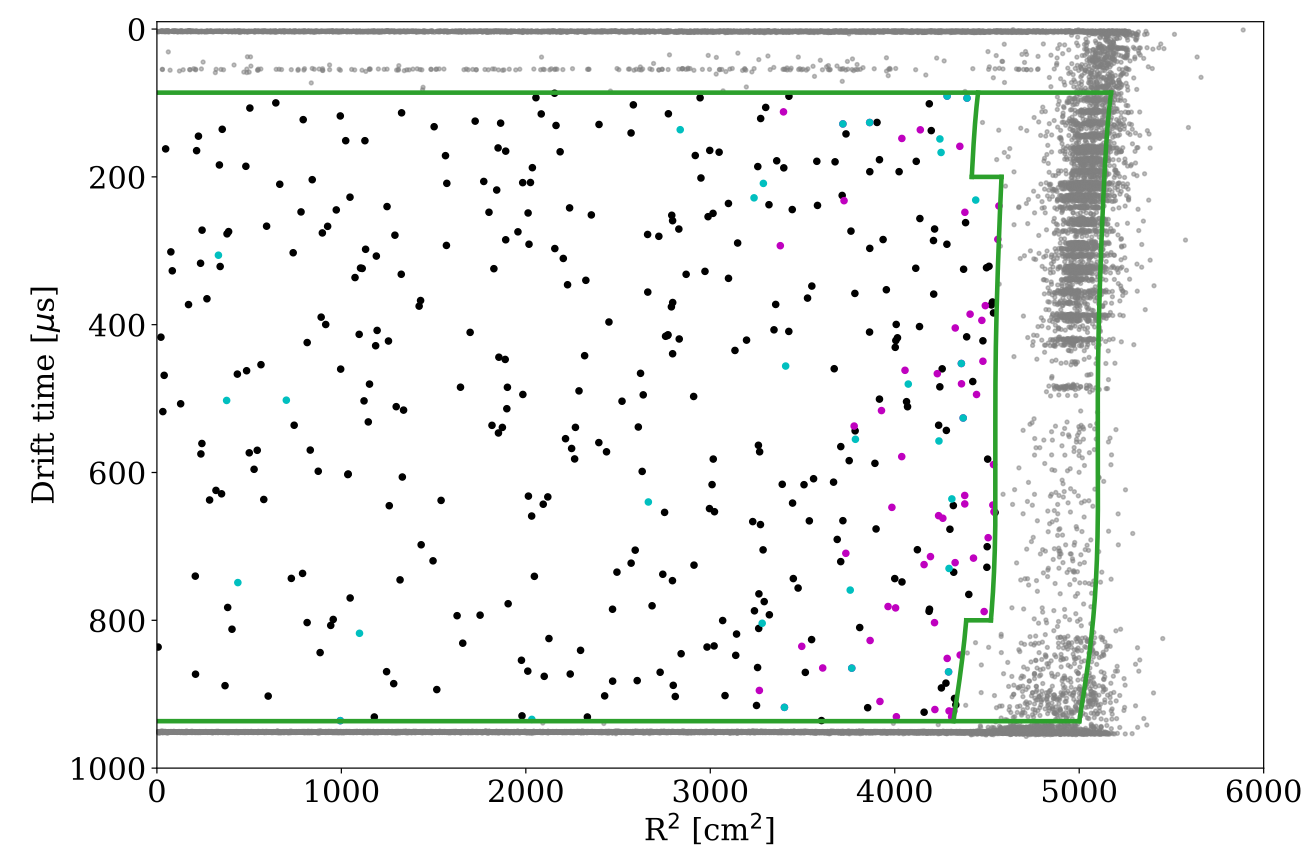
\includegraphics[width=15cm]{Figures/EFT/All_SR1_Plots/fid.png}
%    \caption{Distribution of events in the SR1 dataset in the ROI.
%    The vertical green line which two steps is the fiducial region.
%    The other green line shown is the wall definition.
%    The events in grey are outside of the fiducial volume and so vetoed. 
%    The events marked in cyan were removed by the OD and the events marked in purple by the Skin.
%    The remaining events in the WIMP dataset are shown in black.}
%    \label{fig:sr1_fiducial_cut}
%\end{figure}

\begin{figure}[!htbp]%
\centering
    \begin{tikzpicture}
    \centering
        \begin{groupplot}[view={0}{90},
            group style = {group size = 2 by 1,
            horizontal sep=0.6cm}]
            \nextgroupplot[
            width=0.48\textwidth, height=8cm,
            xlabel={Recoil Energy [keV$_{nr}$]},
            ylabel={S1$_{c}$ [phd]},
            mark size=0pt,
            xmin=0, xmax=100,
            ymin=0, ymax=150]

            \addplot[yellow, name path = psig2] table[x=energy, y=psig2]
                      {Data/HENR/sr1_ws/Signal/data_cuts/s1_vs_recoil.dat};
            \addplot[yellow, name path = nsig2] table[x=energy, y=nsig2]
                      {Data/HENR/sr1_ws/Signal/data_cuts/s1_vs_recoil.dat};
            
            \addplot[green, name path = psig1] table[x=energy, y=psig1]
                      {Data/HENR/sr1_ws/Signal/data_cuts/s1_vs_recoil.dat};
            \addplot[green, name path = nsig1] table[x=energy, y=nsig1]
                      {Data/HENR/sr1_ws/Signal/data_cuts/s1_vs_recoil.dat};
                      
            \addplot[yellow, forget plot] fill between[of=nsig2 and psig2]; 
            \addplot[green, forget plot] fill between[of=nsig1 and psig1];
            
            \addplot[black] table[x=energy, y=mean]
                    {Data/HENR/sr1_ws/Signal/data_cuts/s1_vs_recoil.dat};
            
            \addplot[blue, dashed] coordinates { (0,80)  (100,80)};
            \addplot[black, dashed] coordinates { (72,0)  (72,200)};
                  
            \nextgroupplot[
            width=0.48\textwidth, height=8cm,
            xlabel={Recoil Energy [keV$_{nr}$]},
            ylabel={log$_{10}$(S2$_{c}$ [phd])},
            yticklabel pos=right,
            mark size=0pt,
            xmin=0, xmax=100,
            ymin=2.5, ymax=4.5]
            
            \addplot[yellow, name path = psig2] table[x=energy, y=psig2]
                      {Data/HENR/sr1_ws/Signal/data_cuts/logs2_vs_recoil.dat};
            \addplot[yellow, name path = nsig2] table[x=energy, y=nsig2]
                      {Data/HENR/sr1_ws/Signal/data_cuts/logs2_vs_recoil.dat};
            \addplot[yellow, forget plot] fill between[of=nsig2 and psig2];          
            
            \addplot[green, name path = psig1] table[x=energy, y=psig1]
                      {Data/HENR/sr1_ws/Signal/data_cuts/logs2_vs_recoil.dat};
            \addplot[green, name path = nsig1] table[x=energy, y=nsig1]
                      {Data/HENR/sr1_ws/Signal/data_cuts/logs2_vs_recoil.dat};
            \addplot[green, forget plot] fill between[of=nsig1 and psig1];
            
            \addplot[black] table[x=energy, y=mean]
                    {Data/HENR/sr1_ws/Signal/data_cuts/logs2_vs_recoil.dat};
                    
            \addplot[black, dashed] coordinates { (72,2.5)  (72,4.5)};
        
        \end{groupplot}
    \end{tikzpicture}
    \caption{Detector response in S1 (\textbf{Left}) and S2 (\textbf{Right}) space for a given recoil in the LZ detector for SR1 detector parameters.
    The black line is the mean response, the green band is 1$\sigma$ and the yellow is 3$\sigma$. The blue dashed line is the S1$_c$ cut. The dashed black lines are the largest recoil energy signal within 3$\sigma$ of that cut.
    }
    \label{fig:sr1_detector_model_response_for_flat_nr}
\end{figure}

\begin{figure}
    \centering
    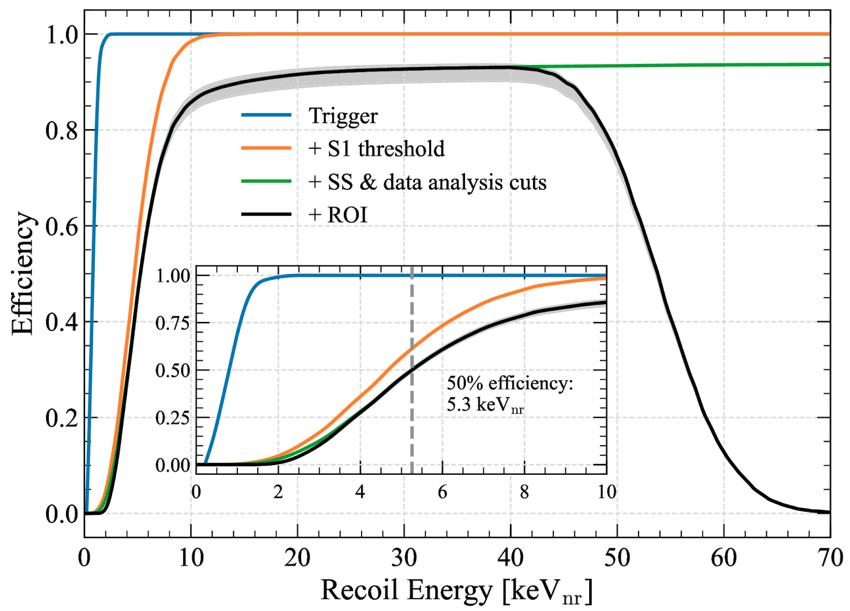
\includegraphics[width=10cm]{Figures/EFT/All_SR1_Plots/NR_efficiency.png}
    \caption{Signal efficiency as a function of NR energy for the trigger (blue), S1 threshold (orange), all analysis cuts expect ROI (green) and the ROI (black).
    The vertical dashed line is the 50\% efficiency point. Figure from \cite{lz_ws_sr1_ref}.
    }
    \label{fig:sr1_nr_efficiency}
\end{figure}

%\begin{figure}[!htbp]%
\centering
\begin{tikzpicture}
\centering
    \begin{axis}[
            ylabel={log${}_{10}$(S2$_c$ [phd])},
            xlabel={S1 [phd]},
            width=15cm,
            height=8cm,
            ymin=2.75, ymax=4.5,
            xmin=0, xmax=80,
            ]
            
        \addplot[gray, opacity = 0.5, fill=gray]
            table [x=x, y=y]
            {Data/HENR/sr1_ws/sr1_data/beta_band_95.dat};
        \addplot[gray, fill=gray]
            table [x=x, y=y]
            {Data/HENR/sr1_ws/sr1_data/beta_band_68.dat};
    
        \addplot[green, opacity = 0.5, fill=green]
            table [x=x, y=y]
            {Data/HENR/sr1_ws/sr1_data/b8_band_95.dat};
        \addplot[green, fill=green]
            table [x=x, y=y]
            {Data/HENR/sr1_ws/sr1_data/b8_band_68.dat};
            
        \addplot[red, ]
            table [x=x, y=y]
            {Data/HENR/sr1_ws/nr_band.dat};    
        \addplot[red, dashed]
            table [x=x, y=high]
            {Data/HENR/sr1_ws/nr_band.dat};     
        \addplot[red, dashed]
            table [x=x, y=low]
            {Data/HENR/sr1_ws/nr_band.dat}; 
            
        \addplot[black, only marks,]
            table [x=S1c, y=log_10S2c]
            {Data/HENR/sr1_ws/ws_data.dat};
            
        \addplot[orange]
            table [x=x, y=y]
            {Data/HENR/sr1_ws/sr1_data/ar37_band_95.dat};
        \addplot[orange]
            table [x=x, y=y]
            {Data/HENR/sr1_ws/sr1_data/ar37_band_68.dat};
    \end{axis}
\end{tikzpicture}
    \caption{SR1 search data after all cuts.}
    \label{fig:henr_ws_sr1_events}
\end{figure}


\subsection{Background Model}
\par
In the background model, 9 components were included listed in \autoref{fig:sr1_er_background_pre_fit}.
The grouping is based on the distribution in the ROI and the level of uncertainty and is discussed below.

\par
In the ROI, there are three dominant $\beta$-decays which make up a flat contribution: ${}^{214}$Pb from the ${}^{222}$Rn chain, ${}^{212}$Pb from the ${}^{220}$Rn chain and ${}^{85}$Kr.
The rate of ${}^{214}$Pb and ${}^{212}$Pb was determined from $\alpha$-peak fitting other decays in the decay chains outside of the ROI \cite{lz_sr1_backgrounds_ref}.
This is analogous to what was shown in \autoref{sec:od_analysis_backgrounds}.
The rate of ${}^{85}$Kr was determined by in situ mass spectroscopy measurements \cite{lz_sr1_backgrounds_ref}. 
%which can be seen in \autoref{fig:sr1_spectra}.
The $\gamma$ spectrum from the detector contaminants is also flat in this region and is constrained from the radioassay \cite{LZ_assay_ref}.
These contributions are treated as a single background labelled \textit{Flat ER} in subsequent plots.
This is the largest contribution to the expected rate, with 218 $\pm$ 36 events.
\par
Two contributions which were ignored in the projected sensitivity have been included here: ${}^{127}$Xe and ${}^{37}$Ar.
As previously discussed, these have half-lives of approximately a month each, and so the contribution during SR1 cannot be ignored.
Both components originate from cosmic activation of xenon, and so the amount of each in the TPC depends upon how long the xenon spent above ground prior to being moved underground.
The contribution from $^{127}$Xe was constrained by sideband analysis from K-shell x-rays deexcitation \cite{marisarthurs_thesis_ref}.
${}^{37}$Ar cannot be constrained by sideband analysis as its decays are entirely within the ROI.
However, the contribution can be constrained by the delivery schedule of the xenon \cite{lz_argon37_ref}.
This put the expected count to be $\approx$100 in this data set, but there is a very large uncertainty meaning that it could be as high as 300.
In the PLR, ${}^{37}$Ar was allowed to float from anywhere between 0 and 291 events \cite{lz_argon37_ref}.
\par
Two other xenon isotopes were considered ${}^{124}$Xe and ${}^{136}$Xe, both of which are constrained by the total mass of xenon \cite{lz_ws_sr1_ref}.
\par
Accidental events, where unrelated S1 and S2 pulses are produced in an event window, were also included in the background model.
The rate of this was determined by the rate of unphysical single scatter events based upon electron drift time \cite{lz_ws_sr1_ref}.
\par
The final ER contribution considered are neutrinos with the rate constrained in the same way as the sensitivity study.
\par
Two contributions to NR events were considered: neutrinos and detector components.
The contribution from NR neutrinos is limited due to the S2$>$600 phd requirement.
Only ${}^{8}$B neutrinos were considered \cite{lz_ws_sr1_ref}.
The rate of neutrons from detector components is constrained by the radioassay and by the number of events which are vetoed by the OD \cite{lz_sr1_backgrounds_ref}.
\par
The background model prior to fitting to the data is shown in \autoref{fig:sr1_er_background_pre_fit}.
The ${}^{37}$Ar component value in the plot uses the post-fit value in the figure. 

\begin{figure}
    \centering
    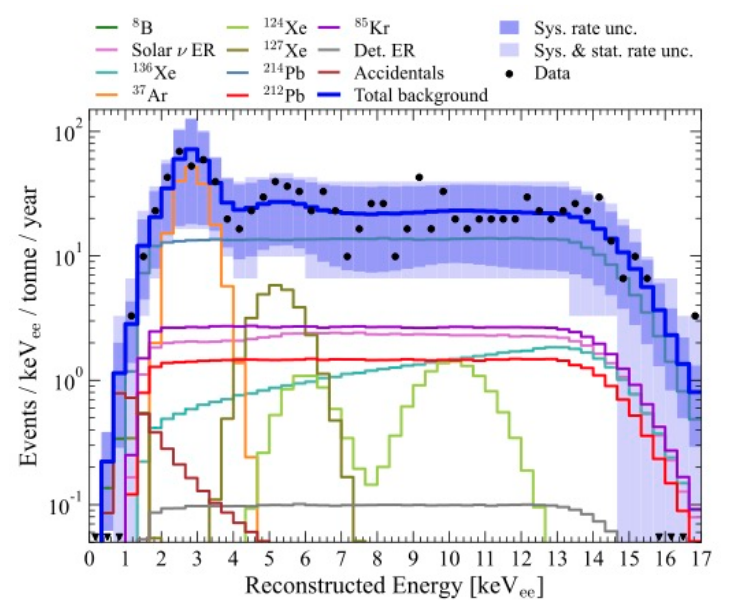
\includegraphics[width=10cm]{Figures/EFT/All_SR1_Plots/sr1_bg_model.png}
    \caption{Background model before fitting to data with the exception of ${}^{37}$Ar, which uses the post-fit rate.
             The total model is shown in dark blue.
             The SR1 data which passed all analysis cuts is shown by the black points.
             Figure from \cite{lz_sr1_backgrounds_ref}.}
    \label{fig:sr1_er_background_pre_fit}
\end{figure}

%\begin{figure}[]%
\centering
\begin{tikzpicture}
\centering
    \begin{axis}[
            ylabel=Rate (/tonne/year/keV),
            xlabel=Reconstructed Energy (keV$_{ee}$),
            width=15cm,
            height=10cm,
            grid=major,
            xmin=80, xmax=700,
            ymin=1e-1, ymax=1e5,
            ymode=log,
            legend style = { column sep = 10pt, legend columns = 2, cells={line width=1.5pt}}
            ]
        \addplot[only marks, mark size=1.0pt, black, error bar legend] 
            plot[error bars/.cd, x dir=both, x explicit, y dir=both, y explicit, ]
            table[x=bin,y=weight,x error=x_error, y error=y_error]
            {Data/HENR/sr1_ws/sr1_data/sr1_background_fit_data.dat};
        \addlegendentry{data};
        
        \addplot[const plot, teal]
            table [x=bins, y=h_bkg_Kr85]
            {Data/HENR/sr1_ws/sr1_data/sr1_background_fit_model.dat};
        \addlegendentry{${}^{85}$Kr};
        
        \addplot[const plot, cyan]
            table [x=bins, y=h_bkg_Pb212]
            {Data/HENR/sr1_ws/sr1_data/sr1_background_fit_model.dat};
        \addlegendentry{${}^{212}$Pb}; 
        
        \addplot[const plot, green]
            table [x=bins, y=h_bkg_Pb214]
            {Data/HENR/sr1_ws/sr1_data/sr1_background_fit_model.dat};
        \addlegendentry{${}^{214}$Pb}; 
        
        \addplot[const plot, lime]
            table [x=bins, y=h_bkg_SolarER]
            {Data/HENR/sr1_ws/sr1_data/sr1_background_fit_model.dat};
        \addlegendentry{Solar ER};
        
        \addplot[const plot, yellow]
            table [x=bins, y=h_bkg_Xe125]
            {Data/HENR/sr1_ws/sr1_data/sr1_background_fit_model.dat};
        \addlegendentry{${}^{125}$Xe};
        
        \addplot[const plot, pink]
            table [x=bins, y=h_bkg_Xe127]
            {Data/HENR/sr1_ws/sr1_data/sr1_background_fit_model.dat};
        \addlegendentry{${}^{127}$Xe};
        
        \addplot[const plot, olive]
            table [x=bins, y=h_bkg_Xe129m]
            {Data/HENR/sr1_ws/sr1_data/sr1_background_fit_model.dat};
        \addlegendentry{${}^{129m}$Xe};
        
        \addplot[const plot, brown]
            table [x=bins, y=h_bkg_Xe131m]
            {Data/HENR/sr1_ws/sr1_data/sr1_background_fit_model.dat};
        \addlegendentry{${}^{131m}$Xe};        

        \addplot[const plot, orange]
            table [x=bins, y=h_bkg_Xe133]
            {Data/HENR/sr1_ws/sr1_data/sr1_background_fit_model.dat};
        \addlegendentry{${}^{133}$Xe};  

        \addplot[const plot, red]
            table [x=bins, y=h_bkg_Xe136]
            {Data/HENR/sr1_ws/sr1_data/sr1_background_fit_model.dat};
        \addlegendentry{${}^{136}$Xe};   
        
        \addplot[const plot, violet]
            table [x=bins, y=h_bkg_full_model]
            {Data/HENR/sr1_ws/sr1_data/sr1_background_fit_model.dat};
        \addlegendentry{model};   
        
\end{axis}
\end{tikzpicture}
    \caption{Result of fit to data.
             \textbf{Top:} Contribution from each source. Only components with a contribution greater than 1 Hz have been included.
             \textbf{Bottom:} Ratio of fit to data. The dashed lines indicate the fit region.
             In generally there is good agreement.}
    \label{fig:sr1_tpc_background_fit_to_data}
\end{figure}



\begin{table}[]
    \centering
    \begin{tabular}{c|c|c}
        Background Component     & Expected Events & Fit Result             \\ \hline
        Flat ER                  & 218 $\pm$ 36    & 222 $\pm$ 16           \\
        $\nu$ ER                 & 27.3 $\pm$ 1.6  & 27.3 $\pm$ 1.6         \\
        ${}^{127}$Xe             & 9.3 $\pm$ 0.8   & 9.3 $\pm$ 0.8          \\
        ${}^{124}$Xe             & 5.0 $\pm$ 1.4   & 5.2 $\pm$ 1.4          \\
        ${}^{136}$Xe             & 15.2 $\pm$ 2.4  & 15.3 $\pm$ 2.4         \\
        ${}^{8}$B CE$\nu$NS      & 0.15 $\pm$ 0.01 & 0.15 $\pm$ 0.01        \\
        Accidentals              & 1.2 $\pm$ 0.3   & 1.2 $\pm$ 0.3          \\
        ${}^{37}$Ar              & [0, 291]        & 52.1${}^{+9.6}_{-8.9}$ \\
        neutrons                 & 0.0${}^{+0.2}$  & 0.0${}^{+0.2}$
    \end{tabular}
    \caption{Number of events from each component in the background model for SR1 before and after the fit.}
    \label{tab:sr1_ws_lz_backgrounds}
\end{table}

%\begin{figure}
%    \centering
%    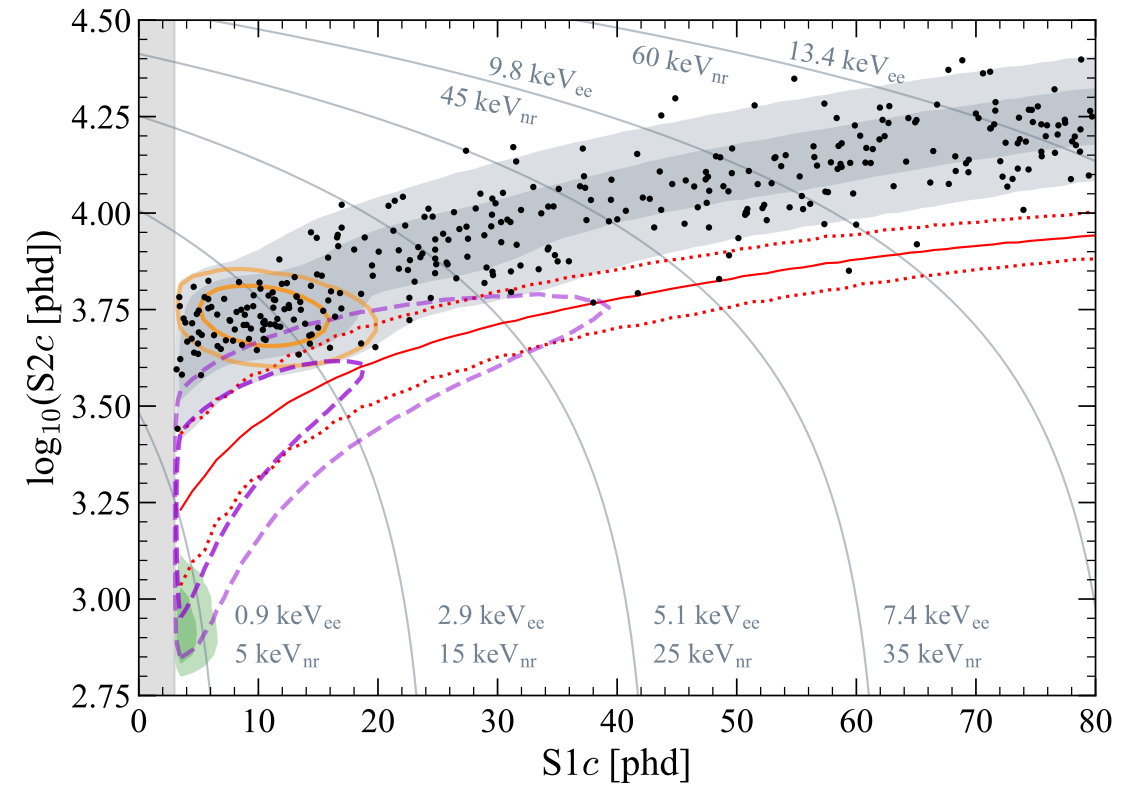
\includegraphics[width=10cm]{Figures/EFT/All_SR1_Plots/final_data_points.png}
%    \caption{SR1 vanilla WIMP-search data (black points) overlaid on the background model.
%    The contours shown for each distribution are 1 and 2 $\sigma$.
%    ${}^{8}$B is shown in green, ${}^{37}$Ar is shown in orange, the combined ER spectrum in grey.
%    The red lines are the NR band with the medium, 10\% and 90\% quantiles.
%    The distribution from a 30 GeV WIMP is also shown in purple. 
%    }
%    \label{fig:final_data_points}
%\end{figure}

\subsection{Signal Model}
\par
The signal models were generated using the recoil spectra described previously in this chapter.
Limiting the maximum recoil energy of 70 keV$_{nr}$ means that some of the operators will have a significant rate outside of the ROI.
Shown in \autoref{tab:sr1_signal_integrated_rates} is the fraction of the total integrated rate for each operator up to 70 keV$_{nr}$ for a number of WIMP masses.
For some operators, as the WIMP mass increases, the rate of recoils decreases significantly, so the sensitivity will be reduced. 


\begin{table}[]
    \centering
    \begin{tabular}{c|c|c|c}
    
        \multirow{2}{*}{Operator} & \multicolumn{3}{c}{Fraction of spectra} \\ 
                                  & 10 GeV/c$^2$ & 100 GeV/c$^2$ & 1000 GeV/c$^2$ \\ \hline
        1                         & 1.0          & 0.997         & 0.993 \\
        3                         & 1.0          & 0.882         & 0.730 \\
        4                         & 1.0          & 0.954         & 0.816 \\
        5                         & 1.0          & 0.942         & 0.736 \\
        6                         & 1.0          & 0.458         & 0.085 \\
        7                         & 1.0          & 0.986         & 0.900 \\
        8                         & 1.0          & 0.991         & 0.963 \\
        9                         & 1.0          & 0.821         & 0.320 \\
        10                        & 1.0          & 0.726         & 0.344 \\
        11                        & 1.0          & 0.986         & 0.949 \\
        12                        & 1.0          & 0.958         & 0.902 \\
        13                        & 1.0          & 0.903         & 0.629 \\
        14                        & 1.0          & 0.859         & 0.359 \\
        15                        & 1.0          & 0.762         & 0.447
    \end{tabular}
    \caption{Fraction of recoil spectra below 70 keV$_{NR}$ for each operator.}
    \label{tab:sr1_signal_integrated_rates}
\end{table}



\subsection{Limits}
\par
On each operator for WIMP masses of [5, 7, 10, 12, 14, 21, 33, 50, 100, 200, 400, 1000, 4000] GeV/c$^2$, a 2-sided frequentist confidence interval is determined above a 90\% confidence level.
Shown in \autoref{tab:sr1_ws_lz_backgrounds} are the constraints and final fit values (from a background-only hypothesis) of the nuisance parameters in this analysis.
This is supported by \autoref{fig:henr_ws_sr1_fitted_events}, which shows the final dataset and the likelihood of each point being part of any given background component.
Many data points have more than one colour, indicating that the background component PDFs overlap.
Each data point is well modelled by the backgrounds considered.

\begin{figure}[]%
\centering
\begin{tikzpicture}
\centering
    \begin{axis}[
            ylabel={log${}_{10}$(S2$_c$ [phd])},
            xlabel={S1 [phd]},
            width=15cm,
            height=8cm,
            ymin=2.75, ymax=4.5,
            xmin=0, xmax=80,
            ]

\draw [black, fill=black] (40.00928,3.98382) -- (40.33150,3.98382) arc [start angle=0.00000,end angle=39.24027, radius=0.05cm] -- (40.00928,3.98382);
\draw [pink, fill=pink] (40.00928,3.98382) -- (40.25884,3.99322) arc [start angle=39.24027,end angle=57.94588, radius=0.05cm] -- (40.00928,3.98382);
\draw [blue, fill=blue] (40.00928,3.98382) -- (40.18029,3.99641) arc [start angle=57.94588,end angle=357.27905, radius=0.05cm] -- (40.00928,3.98382);

\draw [black, fill=black] (12.57129,3.75414) -- (12.89351,3.75414) arc [start angle=0.00000,end angle=10.90037, radius=0.05cm] -- (12.57129,3.75414);
\draw [orange, fill=orange] (12.57129,3.75414) -- (12.88769,3.75695) arc [start angle=10.90037,end angle=257.35718, radius=0.05cm] -- (12.57129,3.75414);
\draw [blue, fill=blue] (12.57129,3.75414) -- (12.50076,3.73964) arc [start angle=257.35718,end angle=356.30690, radius=0.05cm] -- (12.57129,3.75414);

\draw [black, fill=black] (7.28195,3.67028) -- (7.60417,3.67028) arc [start angle=0.00000,end angle=20.52712, radius=0.05cm] -- (7.28195,3.67028);
\draw [orange, fill=orange] (7.28195,3.67028) -- (7.58371,3.67549) arc [start angle=20.52712,end angle=175.25376, radius=0.05cm] -- (7.28195,3.67028);
\draw [blue, fill=blue] (7.28195,3.67028) -- (6.96083,3.67151) arc [start angle=175.25376,end angle=354.73875, radius=0.05cm] -- (7.28195,3.67028);

\draw [black, fill=black] (11.36268,3.71118) -- (11.68490,3.71118) arc [start angle=0.00000,end angle=9.34337, radius=0.05cm] -- (11.36268,3.71118);
\draw [orange, fill=orange] (11.36268,3.71118) -- (11.68063,3.71359) arc [start angle=9.34337,end angle=275.27157, radius=0.05cm] -- (11.36268,3.71118);
\draw [blue, fill=blue] (11.36268,3.71118) -- (11.39228,3.69638) arc [start angle=275.27157,end angle=357.27668, radius=0.05cm] -- (11.36268,3.71118);

\draw [black, fill=black] (62.36395,4.19937) -- (62.68617,4.19937) arc [start angle=0.00000,end angle=35.37095, radius=0.05cm] -- (62.36395,4.19937);
\draw [pink, fill=pink] (62.36395,4.19937) -- (62.62670,4.20797) arc [start angle=35.37095,end angle=63.32370, radius=0.05cm] -- (62.36395,4.19937);
\draw [blue, fill=blue] (62.36395,4.19937) -- (62.50861,4.21265) arc [start angle=63.32370,end angle=359.19930, radius=0.05cm] -- (62.36395,4.19937);

\draw [black, fill=black] (5.80901,3.77719) -- (6.13124,3.77719) arc [start angle=0.00000,end angle=9.11971, radius=0.05cm] -- (5.80901,3.77719);
\draw [orange, fill=orange] (5.80901,3.77719) -- (6.12716,3.77954) arc [start angle=9.11971,end angle=278.91012, radius=0.05cm] -- (5.80901,3.77719);
\draw [blue, fill=blue] (5.80901,3.77719) -- (5.85892,3.76251) arc [start angle=278.91012,end angle=356.87069, radius=0.05cm] -- (5.80901,3.77719);

\draw [black, fill=black] (53.23484,4.14475) -- (53.55706,4.14475) arc [start angle=0.00000,end angle=36.35484, radius=0.05cm] -- (53.23484,4.14475);
\draw [pink, fill=pink] (53.23484,4.14475) -- (53.49434,4.15356) arc [start angle=36.35484,end angle=59.32450, radius=0.05cm] -- (53.23484,4.14475);
\draw [green, fill=green] (53.23484,4.14475) -- (53.39923,4.15753) arc [start angle=59.32450,end angle=74.30965, radius=0.05cm] -- (53.23484,4.14475);
\draw [blue, fill=blue] (53.23484,4.14475) -- (53.32198,4.15906) arc [start angle=74.30965,end angle=359.99542, radius=0.05cm] -- (53.23484,4.14475);

\draw [black, fill=black] (3.74730,3.72675) -- (4.06952,3.72675) arc [start angle=0.00000,end angle=18.46297, radius=0.05cm] -- (3.74730,3.72675);
\draw [pink, fill=pink] (3.74730,3.72675) -- (4.05294,3.73145) arc [start angle=18.46297,end angle=23.52389, radius=0.05cm] -- (3.74730,3.72675);
\draw [orange, fill=orange] (3.74730,3.72675) -- (4.04274,3.73268) arc [start angle=23.52389,end angle=189.71431, radius=0.05cm] -- (3.74730,3.72675);
\draw [blue, fill=blue] (3.74730,3.72675) -- (3.42970,3.72424) arc [start angle=189.71431,end angle=355.38171, radius=0.05cm] -- (3.74730,3.72675);

\draw [black, fill=black] (59.98510,3.97001) -- (60.30732,3.97001) arc [start angle=0.00000,end angle=32.60080, radius=0.05cm] -- (59.98510,3.97001);
\draw [pink, fill=pink] (59.98510,3.97001) -- (60.25655,3.97802) arc [start angle=32.60080,end angle=52.78355, radius=0.05cm] -- (59.98510,3.97001);
\draw [green, fill=green] (59.98510,3.97001) -- (60.17998,3.98184) arc [start angle=52.78355,end angle=87.73142, radius=0.05cm] -- (59.98510,3.97001);
\draw [blue, fill=blue] (59.98510,3.97001) -- (59.99785,3.98486) arc [start angle=87.73142,end angle=359.93131, radius=0.05cm] -- (59.98510,3.97001);

\draw [black, fill=black] (27.40352,3.96478) -- (27.72574,3.96478) arc [start angle=0.00000,end angle=35.53417, radius=0.05cm] -- (27.40352,3.96478);
\draw [pink, fill=pink] (27.40352,3.96478) -- (27.66573,3.97342) arc [start angle=35.53417,end angle=49.80231, radius=0.05cm] -- (27.40352,3.96478);
\draw [green, fill=green] (27.40352,3.96478) -- (27.61149,3.97613) arc [start angle=49.80231,end angle=65.38089, radius=0.05cm] -- (27.40352,3.96478);
\draw [gray, fill=gray] (27.40352,3.96478) -- (27.53775,3.97829) arc [start angle=65.38089,end angle=88.38437, radius=0.05cm] -- (27.40352,3.96478);
\draw [blue, fill=blue] (27.40352,3.96478) -- (27.41260,3.97963) arc [start angle=88.38437,end angle=359.97263, radius=0.05cm] -- (27.40352,3.96478);

\draw [black, fill=black] (74.66848,4.26732) -- (74.99070,4.26732) arc [start angle=0.00000,end angle=35.15746, radius=0.05cm] -- (74.66848,4.26732);
\draw [pink, fill=pink] (74.66848,4.26732) -- (74.93192,4.27588) arc [start angle=35.15746,end angle=68.23490, radius=0.05cm] -- (74.66848,4.26732);
\draw [blue, fill=blue] (74.66848,4.26732) -- (74.78796,4.28112) arc [start angle=68.23490,end angle=359.99853, radius=0.05cm] -- (74.66848,4.26732);

\draw [black, fill=black] (78.26501,4.19843) -- (78.58724,4.19843) arc [start angle=0.00000,end angle=35.21454, radius=0.05cm] -- (78.26501,4.19843);
\draw [pink, fill=pink] (78.26501,4.19843) -- (78.52827,4.20700) arc [start angle=35.21454,end angle=66.47614, radius=0.05cm] -- (78.26501,4.19843);
\draw [blue, fill=blue] (78.26501,4.19843) -- (78.39362,4.21205) arc [start angle=66.47614,end angle=359.99228, radius=0.05cm] -- (78.26501,4.19843);

\draw [black, fill=black] (10.37297,3.69747) -- (10.69520,3.69747) arc [start angle=0.00000,end angle=10.46780, radius=0.05cm] -- (10.37297,3.69747);
\draw [orange, fill=orange] (10.37297,3.69747) -- (10.68983,3.70017) arc [start angle=10.46780,end angle=265.28389, radius=0.05cm] -- (10.37297,3.69747);
\draw [blue, fill=blue] (10.37297,3.69747) -- (10.34648,3.68266) arc [start angle=265.28389,end angle=356.95812, radius=0.05cm] -- (10.37297,3.69747);

\draw [black, fill=black] (25.88875,3.93087) -- (26.21097,3.93087) arc [start angle=0.00000,end angle=32.22008, radius=0.05cm] -- (25.88875,3.93087);
\draw [pink, fill=pink] (25.88875,3.93087) -- (26.16135,3.93879) arc [start angle=32.22008,end angle=44.67690, radius=0.05cm] -- (25.88875,3.93087);
\draw [green, fill=green] (25.88875,3.93087) -- (26.11788,3.94132) arc [start angle=44.67690,end angle=58.56452, radius=0.05cm] -- (25.88875,3.93087);
\draw [gray, fill=gray] (25.88875,3.93087) -- (26.05680,3.94355) arc [start angle=58.56452,end angle=115.55799, radius=0.05cm] -- (25.88875,3.93087);
\draw [blue, fill=blue] (25.88875,3.93087) -- (25.74974,3.94427) arc [start angle=115.55799,end angle=359.97050, radius=0.05cm] -- (25.88875,3.93087);

\draw [black, fill=black] (79.70562,4.25023) -- (80.02784,4.25023) arc [start angle=0.00000,end angle=35.59535, radius=0.05cm] -- (79.70562,4.25023);
\draw [pink, fill=pink] (79.70562,4.25023) -- (79.96763,4.25887) arc [start angle=35.59535,end angle=69.87197, radius=0.05cm] -- (79.70562,4.25023);
\draw [blue, fill=blue] (79.70562,4.25023) -- (79.81650,4.26418) arc [start angle=69.87197,end angle=359.99874, radius=0.05cm] -- (79.70562,4.25023);

\draw [black, fill=black] (25.73676,3.87174) -- (26.05899,3.87174) arc [start angle=0.00000,end angle=27.84138, radius=0.05cm] -- (25.73676,3.87174);
\draw [pink, fill=pink] (25.73676,3.87174) -- (26.02169,3.87868) arc [start angle=27.84138,end angle=38.31557, radius=0.05cm] -- (25.73676,3.87174);
\draw [green, fill=green] (25.73676,3.87174) -- (25.98958,3.88095) arc [start angle=38.31557,end angle=45.84109, radius=0.05cm] -- (25.73676,3.87174);
\draw [gray, fill=gray] (25.73676,3.87174) -- (25.96124,3.88240) arc [start angle=45.84109,end angle=136.13511, radius=0.05cm] -- (25.73676,3.87174);
\draw [blue, fill=blue] (25.73676,3.87174) -- (25.50445,3.88204) arc [start angle=136.13511,end angle=359.96069, radius=0.05cm] -- (25.73676,3.87174);

\draw [black, fill=black] (26.80824,3.95862) -- (27.13046,3.95862) arc [start angle=0.00000,end angle=34.55492, radius=0.05cm] -- (26.80824,3.95862);
\draw [pink, fill=pink] (26.80824,3.95862) -- (27.07362,3.96704) arc [start angle=34.55492,end angle=48.62502, radius=0.05cm] -- (26.80824,3.95862);
\draw [green, fill=green] (26.80824,3.95862) -- (27.02122,3.96976) arc [start angle=48.62502,end angle=63.99245, radius=0.05cm] -- (26.80824,3.95862);
\draw [gray, fill=gray] (26.80824,3.95862) -- (26.94953,3.97197) arc [start angle=63.99245,end angle=95.17134, radius=0.05cm] -- (26.80824,3.95862);
\draw [blue, fill=blue] (26.80824,3.95862) -- (26.77920,3.97341) arc [start angle=95.17134,end angle=359.97128, radius=0.05cm] -- (26.80824,3.95862);

\draw [black, fill=black] (9.06497,3.75501) -- (9.38720,3.75501) arc [start angle=0.00000,end angle=8.83622, radius=0.05cm] -- (9.06497,3.75501);
\draw [orange, fill=orange] (9.06497,3.75501) -- (9.38337,3.75729) arc [start angle=8.83622,end angle=280.04115, radius=0.05cm] -- (9.06497,3.75501);
\draw [blue, fill=blue] (9.06497,3.75501) -- (9.12115,3.74038) arc [start angle=280.04115,end angle=357.30339, radius=0.05cm] -- (9.06497,3.75501);

\draw [black, fill=black] (9.37781,3.70068) -- (9.70003,3.70068) arc [start angle=0.00000,end angle=11.29880, radius=0.05cm] -- (9.37781,3.70068);
\draw [orange, fill=orange] (9.37781,3.70068) -- (9.69378,3.70359) arc [start angle=11.29880,end angle=259.66173, radius=0.05cm] -- (9.37781,3.70068);
\draw [blue, fill=blue] (9.37781,3.70068) -- (9.31998,3.68606) arc [start angle=259.66173,end angle=356.81584, radius=0.05cm] -- (9.37781,3.70068);

\draw [black, fill=black] (57.32886,4.28360) -- (57.65108,4.28360) arc [start angle=0.00000,end angle=35.86768, radius=0.05cm] -- (57.32886,4.28360);
\draw [pink, fill=pink] (57.32886,4.28360) -- (57.58998,4.29231) arc [start angle=35.86768,end angle=66.71942, radius=0.05cm] -- (57.32886,4.28360);
\draw [blue, fill=blue] (57.32886,4.28360) -- (57.45621,4.29725) arc [start angle=66.71942,end angle=359.99174, radius=0.05cm] -- (57.32886,4.28360);

\draw [black, fill=black] (52.15371,4.01296) -- (52.47594,4.01296) arc [start angle=0.00000,end angle=36.77109, radius=0.05cm] -- (52.15371,4.01296);
\draw [pink, fill=pink] (52.15371,4.01296) -- (52.41182,4.02186) arc [start angle=36.77109,end angle=57.69711, radius=0.05cm] -- (52.15371,4.01296);
\draw [green, fill=green] (52.15371,4.01296) -- (52.32591,4.02552) arc [start angle=57.69711,end angle=76.66904, radius=0.05cm] -- (52.15371,4.01296);
\draw [blue, fill=blue] (52.15371,4.01296) -- (52.22801,4.02742) arc [start angle=76.66904,end angle=359.98561, radius=0.05cm] -- (52.15371,4.01296);

\draw [black, fill=black] (72.62480,4.06848) -- (72.94702,4.06848) arc [start angle=0.00000,end angle=35.73618, radius=0.05cm] -- (72.62480,4.06848);
\draw [pink, fill=pink] (72.62480,4.06848) -- (72.88635,4.07716) arc [start angle=35.73618,end angle=61.45395, radius=0.05cm] -- (72.62480,4.06848);
\draw [green, fill=green] (72.62480,4.06848) -- (72.77878,4.08153) arc [start angle=61.45395,end angle=73.28572, radius=0.05cm] -- (72.62480,4.06848);
\draw [blue, fill=blue] (72.62480,4.06848) -- (72.71747,4.08271) arc [start angle=73.28572,end angle=359.98488, radius=0.05cm] -- (72.62480,4.06848);

\draw [black, fill=black] (30.30806,3.92453) -- (30.63028,3.92453) arc [start angle=0.00000,end angle=33.76827, radius=0.05cm] -- (30.30806,3.92453);
\draw [pink, fill=pink] (30.30806,3.92453) -- (30.57592,3.93278) arc [start angle=33.76827,end angle=47.00413, radius=0.05cm] -- (30.30806,3.92453);
\draw [green, fill=green] (30.30806,3.92453) -- (30.52779,3.93539) arc [start angle=47.00413,end angle=66.33596, radius=0.05cm] -- (30.30806,3.92453);
\draw [gray, fill=gray] (30.30806,3.92453) -- (30.43739,3.93813) arc [start angle=66.33596,end angle=104.95340, radius=0.05cm] -- (30.30806,3.92453);
\draw [blue, fill=blue] (30.30806,3.92453) -- (30.22491,3.93888) arc [start angle=104.95340,end angle=359.97399, radius=0.05cm] -- (30.30806,3.92453);

\draw [black, fill=black] (56.48796,4.14503) -- (56.81018,4.14503) arc [start angle=0.00000,end angle=35.29636, radius=0.05cm] -- (56.48796,4.14503);
\draw [pink, fill=pink] (56.48796,4.14503) -- (56.75095,4.15362) arc [start angle=35.29636,end angle=60.04975, radius=0.05cm] -- (56.48796,4.14503);
\draw [green, fill=green] (56.48796,4.14503) -- (56.64883,4.15790) arc [start angle=60.04975,end angle=72.77544, radius=0.05cm] -- (56.48796,4.14503);
\draw [blue, fill=blue] (56.48796,4.14503) -- (56.58338,4.15922) arc [start angle=72.77544,end angle=359.99609, radius=0.05cm] -- (56.48796,4.14503);

\draw [black, fill=black] (14.30739,3.66165) -- (14.62961,3.66165) arc [start angle=0.00000,end angle=9.88354, radius=0.05cm] -- (14.30739,3.66165);
\draw [orange, fill=orange] (14.30739,3.66165) -- (14.62483,3.66420) arc [start angle=9.88354,end angle=270.92869, radius=0.05cm] -- (14.30739,3.66165);
\draw [blue, fill=blue] (14.30739,3.66165) -- (14.31261,3.64680) arc [start angle=270.92869,end angle=357.08275, radius=0.05cm] -- (14.30739,3.66165);

\draw [black, fill=black] (45.63678,3.97239) -- (45.95901,3.97239) arc [start angle=0.00000,end angle=37.04823, radius=0.05cm] -- (45.63678,3.97239);
\draw [pink, fill=pink] (45.63678,3.97239) -- (45.89396,3.98134) arc [start angle=37.04823,end angle=56.07428, radius=0.05cm] -- (45.63678,3.97239);
\draw [blue, fill=blue] (45.63678,3.97239) -- (45.81662,3.98472) arc [start angle=56.07428,end angle=356.92672, radius=0.05cm] -- (45.63678,3.97239);

\draw [black, fill=black] (14.39964,3.95009) -- (14.72186,3.95009) arc [start angle=0.00000,end angle=33.40257, radius=0.05cm] -- (14.39964,3.95009);
\draw [pink, fill=pink] (14.39964,3.95009) -- (14.66864,3.95827) arc [start angle=33.40257,end angle=45.45729, radius=0.05cm] -- (14.39964,3.95009);
\draw [gray, fill=gray] (14.39964,3.95009) -- (14.62566,3.96068) arc [start angle=45.45729,end angle=90.77698, radius=0.05cm] -- (14.39964,3.95009);
\draw [blue, fill=blue] (14.39964,3.95009) -- (14.39527,3.96495) arc [start angle=90.77698,end angle=357.87644, radius=0.05cm] -- (14.39964,3.95009);

\draw [black, fill=black] (24.41422,3.78011) -- (24.73644,3.78011) arc [start angle=0.00000,end angle=31.22533, radius=0.05cm] -- (24.41422,3.78011);
\draw [pink, fill=pink] (24.41422,3.78011) -- (24.68976,3.78782) arc [start angle=31.22533,end angle=42.51590, radius=0.05cm] -- (24.41422,3.78011);
\draw [gray, fill=gray] (24.41422,3.78011) -- (24.65173,3.79015) arc [start angle=42.51590,end angle=100.84322, radius=0.05cm] -- (24.41422,3.78011);
\draw [blue, fill=blue] (24.41422,3.78011) -- (24.35360,3.79471) arc [start angle=100.84322,end angle=356.29243, radius=0.05cm] -- (24.41422,3.78011);

\draw [black, fill=black] (11.19674,3.79452) -- (11.51897,3.79452) arc [start angle=0.00000,end angle=14.24280, radius=0.05cm] -- (11.19674,3.79452);
\draw [orange, fill=orange] (11.19674,3.79452) -- (11.50906,3.79818) arc [start angle=14.24280,end angle=230.19119, radius=0.05cm] -- (11.19674,3.79452);
\draw [blue, fill=blue] (11.19674,3.79452) -- (10.99045,3.78311) arc [start angle=230.19119,end angle=355.33112, radius=0.05cm] -- (11.19674,3.79452);

\draw [black, fill=black] (33.65458,3.99933) -- (33.97680,3.99933) arc [start angle=0.00000,end angle=38.35134, radius=0.05cm] -- (33.65458,3.99933);
\draw [pink, fill=pink] (33.65458,3.99933) -- (33.90727,4.00855) arc [start angle=38.35134,end angle=56.43238, radius=0.05cm] -- (33.65458,3.99933);
\draw [blue, fill=blue] (33.65458,3.99933) -- (33.83274,4.01171) arc [start angle=56.43238,end angle=353.99261, radius=0.05cm] -- (33.65458,3.99933);

\draw [black, fill=black] (13.91094,3.71338) -- (14.23316,3.71338) arc [start angle=0.00000,end angle=10.08942, radius=0.05cm] -- (13.91094,3.71338);
\draw [orange, fill=orange] (13.91094,3.71338) -- (14.22817,3.71598) arc [start angle=10.08942,end angle=268.79732, radius=0.05cm] -- (13.91094,3.71338);
\draw [blue, fill=blue] (13.91094,3.71338) -- (13.90417,3.69852) arc [start angle=268.79732,end angle=356.87104, radius=0.05cm] -- (13.91094,3.71338);

\draw [black, fill=black] (8.17713,3.74377) -- (8.49935,3.74377) arc [start angle=0.00000,end angle=9.46148, radius=0.05cm] -- (8.17713,3.74377);
\draw [orange, fill=orange] (8.17713,3.74377) -- (8.49496,3.74622) arc [start angle=9.46148,end angle=275.16549, radius=0.05cm] -- (8.17713,3.74377);
\draw [blue, fill=blue] (8.17713,3.74377) -- (8.20614,3.72898) arc [start angle=275.16549,end angle=357.21624, radius=0.05cm] -- (8.17713,3.74377);

\draw [black, fill=black] (36.89751,4.06951) -- (37.21973,4.06951) arc [start angle=0.00000,end angle=38.88888, radius=0.05cm] -- (36.89751,4.06951);
\draw [pink, fill=pink] (36.89751,4.06951) -- (37.14832,4.07884) arc [start angle=38.88888,end angle=58.32781, radius=0.05cm] -- (36.89751,4.06951);
\draw [blue, fill=blue] (36.89751,4.06951) -- (37.06670,4.08215) arc [start angle=58.32781,end angle=358.29037, radius=0.05cm] -- (36.89751,4.06951);

\draw [black, fill=black] (47.69737,4.05776) -- (48.01959,4.05776) arc [start angle=0.00000,end angle=37.79022, radius=0.05cm] -- (47.69737,4.05776);
\draw [pink, fill=pink] (47.69737,4.05776) -- (47.95201,4.06686) arc [start angle=37.79022,end angle=58.88347, radius=0.05cm] -- (47.69737,4.05776);
\draw [green, fill=green] (47.69737,4.05776) -- (47.86389,4.07048) arc [start angle=58.88347,end angle=73.60204, radius=0.05cm] -- (47.69737,4.05776);
\draw [blue, fill=blue] (47.69737,4.05776) -- (47.78833,4.07201) arc [start angle=73.60204,end angle=359.99194, radius=0.05cm] -- (47.69737,4.05776);

\draw [black, fill=black] (27.36173,4.16159) -- (27.68395,4.16159) arc [start angle=0.00000,end angle=39.15732, radius=0.05cm] -- (27.36173,4.16159);
\draw [pink, fill=pink] (27.36173,4.16159) -- (27.61158,4.17097) arc [start angle=39.15732,end angle=57.15222, radius=0.05cm] -- (27.36173,4.16159);
\draw [blue, fill=blue] (27.36173,4.16159) -- (27.53650,4.17407) arc [start angle=57.15222,end angle=359.06932, radius=0.05cm] -- (27.36173,4.16159);

\draw [black, fill=black] (38.00267,3.76806) -- (38.32489,3.76806) arc [start angle=0.00000,end angle=23.34068, radius=0.05cm] -- (38.00267,3.76806);
\draw [pink, fill=pink] (38.00267,3.76806) -- (38.29852,3.77395) arc [start angle=23.34068,end angle=32.22509, radius=0.05cm] -- (38.00267,3.76806);
\draw [green, fill=green] (38.00267,3.76806) -- (38.27526,3.77599) arc [start angle=32.22509,end angle=62.04172, radius=0.05cm] -- (38.00267,3.76806);
\draw [gray, fill=gray] (38.00267,3.76806) -- (38.15374,3.78119) arc [start angle=62.04172,end angle=176.67875, radius=0.05cm] -- (38.00267,3.76806);
\draw [blue, fill=blue] (38.00267,3.76806) -- (37.68099,3.76893) arc [start angle=176.67875,end angle=358.91552, radius=0.05cm] -- (38.00267,3.76806);

\draw [black, fill=black] (59.48688,4.13005) -- (59.80910,4.13005) arc [start angle=0.00000,end angle=36.07861, radius=0.05cm] -- (59.48688,4.13005);
\draw [pink, fill=pink] (59.48688,4.13005) -- (59.74730,4.13880) arc [start angle=36.07861,end angle=60.59168, radius=0.05cm] -- (59.48688,4.13005);
\draw [green, fill=green] (59.48688,4.13005) -- (59.64510,4.14299) arc [start angle=60.59168,end angle=73.56489, radius=0.05cm] -- (59.48688,4.13005);
\draw [blue, fill=blue] (59.48688,4.13005) -- (59.57804,4.14430) arc [start angle=73.56489,end angle=359.99593, radius=0.05cm] -- (59.48688,4.13005);

\draw [black, fill=black] (29.53017,3.99585) -- (29.85239,3.99585) arc [start angle=0.00000,end angle=37.73687, radius=0.05cm] -- (29.53017,3.99585);
\draw [pink, fill=pink] (29.53017,3.99585) -- (29.78499,4.00494) arc [start angle=37.73687,end angle=54.74631, radius=0.05cm] -- (29.53017,3.99585);
\draw [green, fill=green] (29.53017,3.99585) -- (29.71615,4.00798) arc [start angle=54.74631,end angle=63.91207, radius=0.05cm] -- (29.53017,3.99585);
\draw [blue, fill=blue] (29.53017,3.99585) -- (29.67187,4.00919) arc [start angle=63.91207,end angle=355.88105, radius=0.05cm] -- (29.53017,3.99585);

\draw [black, fill=black] (13.03509,3.83414) -- (13.35731,3.83414) arc [start angle=0.00000,end angle=27.53499, radius=0.05cm] -- (13.03509,3.83414);
\draw [pink, fill=pink] (13.03509,3.83414) -- (13.32082,3.84101) arc [start angle=27.53499,end angle=36.78957, radius=0.05cm] -- (13.03509,3.83414);
\draw [orange, fill=orange] (13.03509,3.83414) -- (13.29314,3.84304) arc [start angle=36.78957,end angle=108.53545, radius=0.05cm] -- (13.03509,3.83414);
\draw [blue, fill=blue] (13.03509,3.83414) -- (12.93266,3.84823) arc [start angle=108.53545,end angle=357.45637, radius=0.05cm] -- (13.03509,3.83414);

\draw [black, fill=black] (53.71547,4.12159) -- (54.03769,4.12159) arc [start angle=0.00000,end angle=35.67012, radius=0.05cm] -- (53.71547,4.12159);
\draw [pink, fill=pink] (53.71547,4.12159) -- (53.97724,4.13025) arc [start angle=35.67012,end angle=58.95723, radius=0.05cm] -- (53.71547,4.12159);
\draw [green, fill=green] (53.71547,4.12159) -- (53.88163,4.13432) arc [start angle=58.95723,end angle=80.23885, radius=0.05cm] -- (53.71547,4.12159);
\draw [blue, fill=blue] (53.71547,4.12159) -- (53.77010,4.13623) arc [start angle=80.23885,end angle=359.99504, radius=0.05cm] -- (53.71547,4.12159);

\draw [black, fill=black] (58.67392,4.12733) -- (58.99614,4.12733) arc [start angle=0.00000,end angle=35.91110, radius=0.05cm] -- (58.67392,4.12733);
\draw [pink, fill=pink] (58.67392,4.12733) -- (58.93490,4.13604) arc [start angle=35.91110,end angle=60.17064, radius=0.05cm] -- (58.67392,4.12733);
\draw [green, fill=green] (58.67392,4.12733) -- (58.83420,4.14022) arc [start angle=60.17064,end angle=74.94938, radius=0.05cm] -- (58.67392,4.12733);
\draw [blue, fill=blue] (58.67392,4.12733) -- (58.75759,4.14168) arc [start angle=74.94938,end angle=359.99574, radius=0.05cm] -- (58.67392,4.12733);

\draw [black, fill=black] (56.71368,4.12304) -- (57.03591,4.12304) arc [start angle=0.00000,end angle=35.12492, radius=0.05cm] -- (56.71368,4.12304);
\draw [pink, fill=pink] (56.71368,4.12304) -- (56.97723,4.13158) arc [start angle=35.12492,end angle=58.45088, radius=0.05cm] -- (56.71368,4.12304);
\draw [green, fill=green] (56.71368,4.12304) -- (56.88228,4.13570) arc [start angle=58.45088,end angle=77.44122, radius=0.05cm] -- (56.71368,4.12304);
\draw [blue, fill=blue] (56.71368,4.12304) -- (56.78375,4.13754) arc [start angle=77.44122,end angle=359.99562, radius=0.05cm] -- (56.71368,4.12304);

\draw [black, fill=black] (22.08357,4.04218) -- (22.40580,4.04218) arc [start angle=0.00000,end angle=38.30886, radius=0.05cm] -- (22.08357,4.04218);
\draw [pink, fill=pink] (22.08357,4.04218) -- (22.33642,4.05139) arc [start angle=38.30886,end angle=54.66832, radius=0.05cm] -- (22.08357,4.04218);
\draw [green, fill=green] (22.08357,4.04218) -- (22.26992,4.05430) arc [start angle=54.66832,end angle=61.88834, radius=0.05cm] -- (22.08357,4.04218);
\draw [gray, fill=gray] (22.08357,4.04218) -- (22.23540,4.05529) arc [start angle=61.88834,end angle=67.97837, radius=0.05cm] -- (22.08357,4.04218);
\draw [blue, fill=blue] (22.08357,4.04218) -- (22.20439,4.05596) arc [start angle=67.97837,end angle=359.84745, radius=0.05cm] -- (22.08357,4.04218);

\draw [black, fill=black] (9.87382,3.64493) -- (10.19604,3.64493) arc [start angle=0.00000,end angle=16.91809, radius=0.05cm] -- (9.87382,3.64493);
\draw [orange, fill=orange] (9.87382,3.64493) -- (10.18209,3.64925) arc [start angle=16.91809,end angle=207.44135, radius=0.05cm] -- (9.87382,3.64493);
\draw [blue, fill=blue] (9.87382,3.64493) -- (9.58785,3.63808) arc [start angle=207.44135,end angle=355.24265, radius=0.05cm] -- (9.87382,3.64493);

\draw [black, fill=black] (6.59143,3.65534) -- (6.91366,3.65534) arc [start angle=0.00000,end angle=26.13297, radius=0.05cm] -- (6.59143,3.65534);
\draw [pink, fill=pink] (6.59143,3.65534) -- (6.88072,3.66188) arc [start angle=26.13297,end angle=32.37046, radius=0.05cm] -- (6.59143,3.65534);
\draw [orange, fill=orange] (6.59143,3.65534) -- (6.86358,3.66329) arc [start angle=32.37046,end angle=133.15427, radius=0.05cm] -- (6.59143,3.65534);
\draw [blue, fill=blue] (6.59143,3.65534) -- (6.37104,3.66618) arc [start angle=133.15427,end angle=359.17986, radius=0.05cm] -- (6.59143,3.65534);

\draw [black, fill=black] (57.40655,4.05558) -- (57.72877,4.05558) arc [start angle=0.00000,end angle=34.38003, radius=0.05cm] -- (57.40655,4.05558);
\draw [pink, fill=pink] (57.40655,4.05558) -- (57.67248,4.06397) arc [start angle=34.38003,end angle=55.73599, radius=0.05cm] -- (57.40655,4.05558);
\draw [green, fill=green] (57.40655,4.05558) -- (57.58796,4.06786) arc [start angle=55.73599,end angle=87.37920, radius=0.05cm] -- (57.40655,4.05558);
\draw [blue, fill=blue] (57.40655,4.05558) -- (57.42129,4.07042) arc [start angle=87.37920,end angle=359.99179, radius=0.05cm] -- (57.40655,4.05558);

\draw [black, fill=black] (9.21492,3.67386) -- (9.53714,3.67386) arc [start angle=0.00000,end angle=14.42225, radius=0.05cm] -- (9.21492,3.67386);
\draw [orange, fill=orange] (9.21492,3.67386) -- (9.52699,3.67756) arc [start angle=14.42225,end angle=230.33400, radius=0.05cm] -- (9.21492,3.67386);
\draw [blue, fill=blue] (9.21492,3.67386) -- (9.00924,3.66242) arc [start angle=230.33400,end angle=355.89140, radius=0.05cm] -- (9.21492,3.67386);

\draw [black, fill=black] (11.58248,3.72569) -- (11.90470,3.72569) arc [start angle=0.00000,end angle=9.10591, radius=0.05cm] -- (11.58248,3.72569);
\draw [orange, fill=orange] (11.58248,3.72569) -- (11.90064,3.72804) arc [start angle=9.10591,end angle=276.89355, radius=0.05cm] -- (11.58248,3.72569);
\draw [blue, fill=blue] (11.58248,3.72569) -- (11.62115,3.71094) arc [start angle=276.89355,end angle=357.32541, radius=0.05cm] -- (11.58248,3.72569);

\draw [black, fill=black] (4.46028,3.71452) -- (4.78250,3.71452) arc [start angle=0.00000,end angle=19.63519, radius=0.05cm] -- (4.46028,3.71452);
\draw [pink, fill=pink] (4.46028,3.71452) -- (4.76376,3.71952) arc [start angle=19.63519,end angle=24.78508, radius=0.05cm] -- (4.46028,3.71452);
\draw [orange, fill=orange] (4.46028,3.71452) -- (4.75282,3.72075) arc [start angle=24.78508,end angle=182.37259, radius=0.05cm] -- (4.46028,3.71452);
\draw [blue, fill=blue] (4.46028,3.71452) -- (4.13833,3.71391) arc [start angle=182.37259,end angle=358.02690, radius=0.05cm] -- (4.46028,3.71452);

\draw [black, fill=black] (8.76765,3.70998) -- (9.08987,3.70998) arc [start angle=0.00000,end angle=11.01540, radius=0.05cm] -- (8.76765,3.70998);
\draw [orange, fill=orange] (8.76765,3.70998) -- (9.08394,3.71282) arc [start angle=11.01540,end angle=260.42991, radius=0.05cm] -- (8.76765,3.70998);
\draw [blue, fill=blue] (8.76765,3.70998) -- (8.71408,3.69533) arc [start angle=260.42991,end angle=356.79437, radius=0.05cm] -- (8.76765,3.70998);

\draw [black, fill=black] (10.97286,3.71182) -- (11.29509,3.71182) arc [start angle=0.00000,end angle=9.40940, radius=0.05cm] -- (10.97286,3.71182);
\draw [orange, fill=orange] (10.97286,3.71182) -- (11.29075,3.71425) arc [start angle=9.40940,end angle=273.99308, radius=0.05cm] -- (10.97286,3.71182);
\draw [blue, fill=blue] (10.97286,3.71182) -- (10.99530,3.69700) arc [start angle=273.99308,end angle=357.22229, radius=0.05cm] -- (10.97286,3.71182);

\draw [black, fill=black] (8.03131,3.69842) -- (8.35353,3.69842) arc [start angle=0.00000,end angle=13.49889, radius=0.05cm] -- (8.03131,3.69842);
\draw [orange, fill=orange] (8.03131,3.69842) -- (8.34463,3.70189) arc [start angle=13.49889,end angle=238.26803, radius=0.05cm] -- (8.03131,3.69842);
\draw [blue, fill=blue] (8.03131,3.69842) -- (7.86184,3.68579) arc [start angle=238.26803,end angle=356.07376, radius=0.05cm] -- (8.03131,3.69842);

\draw [black, fill=black] (7.88370,3.66925) -- (8.20592,3.66925) arc [start angle=0.00000,end angle=18.84544, radius=0.05cm] -- (7.88370,3.66925);
\draw [orange, fill=orange] (7.88370,3.66925) -- (8.18864,3.67405) arc [start angle=18.84544,end angle=189.83197, radius=0.05cm] -- (7.88370,3.66925);
\draw [blue, fill=blue] (7.88370,3.66925) -- (7.56621,3.66672) arc [start angle=189.83197,end angle=355.06417, radius=0.05cm] -- (7.88370,3.66925);

\draw [black, fill=black] (10.85406,3.78625) -- (11.17628,3.78625) arc [start angle=0.00000,end angle=12.57515, radius=0.05cm] -- (10.85406,3.78625);
\draw [orange, fill=orange] (10.85406,3.78625) -- (11.16855,3.78949) arc [start angle=12.57515,end angle=246.09901, radius=0.05cm] -- (10.85406,3.78625);
\draw [blue, fill=blue] (10.85406,3.78625) -- (10.72351,3.77267) arc [start angle=246.09901,end angle=356.01970, radius=0.05cm] -- (10.85406,3.78625);

\draw [black, fill=black] (24.21967,4.01133) -- (24.54189,4.01133) arc [start angle=0.00000,end angle=37.17218, radius=0.05cm] -- (24.21967,4.01133);
\draw [pink, fill=pink] (24.21967,4.01133) -- (24.47642,4.02031) arc [start angle=37.17218,end angle=52.66992, radius=0.05cm] -- (24.21967,4.01133);
\draw [green, fill=green] (24.21967,4.01133) -- (24.41507,4.02314) arc [start angle=52.66992,end angle=63.80098, radius=0.05cm] -- (24.21967,4.01133);
\draw [gray, fill=gray] (24.21967,4.01133) -- (24.36193,4.02466) arc [start angle=63.80098,end angle=75.71657, radius=0.05cm] -- (24.21967,4.01133);
\draw [blue, fill=blue] (24.21967,4.01133) -- (24.29917,4.02573) arc [start angle=75.71657,end angle=359.93982, radius=0.05cm] -- (24.21967,4.01133);

\draw [black, fill=black] (47.49152,4.02644) -- (47.81374,4.02644) arc [start angle=0.00000,end angle=36.64019, radius=0.05cm] -- (47.49152,4.02644);
\draw [pink, fill=pink] (47.49152,4.02644) -- (47.75007,4.03531) arc [start angle=36.64019,end angle=57.01917, radius=0.05cm] -- (47.49152,4.02644);
\draw [green, fill=green] (47.49152,4.02644) -- (47.66692,4.03890) arc [start angle=57.01917,end angle=66.19605, radius=0.05cm] -- (47.49152,4.02644);
\draw [blue, fill=blue] (47.49152,4.02644) -- (47.62157,4.04004) arc [start angle=66.19605,end angle=359.98748, radius=0.05cm] -- (47.49152,4.02644);

\draw [black, fill=black] (13.18465,3.78420) -- (13.50687,3.78420) arc [start angle=0.00000,end angle=16.89647, radius=0.05cm] -- (13.18465,3.78420);
\draw [pink, fill=pink] (13.18465,3.78420) -- (13.49296,3.78852) arc [start angle=16.89647,end angle=22.30110, radius=0.05cm] -- (13.18465,3.78420);
\draw [orange, fill=orange] (13.18465,3.78420) -- (13.48277,3.78984) arc [start angle=22.30110,end angle=210.72307, radius=0.05cm] -- (13.18465,3.78420);
\draw [blue, fill=blue] (13.18465,3.78420) -- (12.90765,3.77661) arc [start angle=210.72307,end angle=359.63208, radius=0.05cm] -- (13.18465,3.78420);

\draw [black, fill=black] (71.61829,4.26542) -- (71.94051,4.26542) arc [start angle=0.00000,end angle=36.14616, radius=0.05cm] -- (71.61829,4.26542);
\draw [pink, fill=pink] (71.61829,4.26542) -- (71.87849,4.27418) arc [start angle=36.14616,end angle=69.01468, radius=0.05cm] -- (71.61829,4.26542);
\draw [blue, fill=blue] (71.61829,4.26542) -- (71.73368,4.27929) arc [start angle=69.01468,end angle=359.99827, radius=0.05cm] -- (71.61829,4.26542);

\draw [black, fill=black] (3.43062,3.75886) -- (3.75285,3.75886) arc [start angle=0.00000,end angle=12.77518, radius=0.05cm] -- (3.43062,3.75886);
\draw [orange, fill=orange] (3.43062,3.75886) -- (3.74487,3.76215) arc [start angle=12.77518,end angle=233.86793, radius=0.05cm] -- (3.43062,3.75886);
\draw [blue, fill=blue] (3.43062,3.75886) -- (3.24063,3.74686) arc [start angle=233.86793,end angle=349.85459, radius=0.05cm] -- (3.43062,3.75886);
\draw [purple, fill=purple] (3.43062,3.75886) -- (3.74781,3.75624) arc [start angle=349.85459,end angle=356.73763, radius=0.05cm] -- (3.43062,3.75886);

\draw [black, fill=black] (78.04781,4.18581) -- (78.37004,4.18581) arc [start angle=0.00000,end angle=35.78618, radius=0.05cm] -- (78.04781,4.18581);
\draw [pink, fill=pink] (78.04781,4.18581) -- (78.30920,4.19449) arc [start angle=35.78618,end angle=66.15768, radius=0.05cm] -- (78.04781,4.18581);
\draw [blue, fill=blue] (78.04781,4.18581) -- (78.17806,4.19940) arc [start angle=66.15768,end angle=359.97922, radius=0.05cm] -- (78.04781,4.18581);

\draw [black, fill=black] (75.50079,4.14713) -- (75.82302,4.14713) arc [start angle=0.00000,end angle=35.48602, radius=0.05cm] -- (75.50079,4.14713);
\draw [pink, fill=pink] (75.50079,4.14713) -- (75.76317,4.15575) arc [start angle=35.48602,end angle=64.03563, radius=0.05cm] -- (75.50079,4.14713);
\draw [blue, fill=blue] (75.50079,4.14713) -- (75.64187,4.16049) arc [start angle=64.03563,end angle=359.66558, radius=0.05cm] -- (75.50079,4.14713);

\draw [black, fill=black] (13.50055,3.76973) -- (13.82277,3.76973) arc [start angle=0.00000,end angle=14.54819, radius=0.05cm] -- (13.50055,3.76973);
\draw [orange, fill=orange] (13.50055,3.76973) -- (13.81244,3.77346) arc [start angle=14.54819,end angle=224.17330, radius=0.05cm] -- (13.50055,3.76973);
\draw [blue, fill=blue] (13.50055,3.76973) -- (13.26944,3.75937) arc [start angle=224.17330,end angle=354.95742, radius=0.05cm] -- (13.50055,3.76973);

\draw [black, fill=black] (13.21194,3.78294) -- (13.53416,3.78294) arc [start angle=0.00000,end angle=16.65484, radius=0.05cm] -- (13.21194,3.78294);
\draw [pink, fill=pink] (13.21194,3.78294) -- (13.52064,3.78720) arc [start angle=16.65484,end angle=22.00008, radius=0.05cm] -- (13.21194,3.78294);
\draw [orange, fill=orange] (13.21194,3.78294) -- (13.51069,3.78851) arc [start angle=22.00008,end angle=212.47722, radius=0.05cm] -- (13.21194,3.78294);
\draw [blue, fill=blue] (13.21194,3.78294) -- (12.94011,3.77496) arc [start angle=212.47722,end angle=359.63995, radius=0.05cm] -- (13.21194,3.78294);

\draw [black, fill=black] (69.39980,4.13815) -- (69.72203,4.13815) arc [start angle=0.00000,end angle=36.17046, radius=0.05cm] -- (69.39980,4.13815);
\draw [pink, fill=pink] (69.39980,4.13815) -- (69.65992,4.14692) arc [start angle=36.17046,end angle=64.54159, radius=0.05cm] -- (69.39980,4.13815);
\draw [blue, fill=blue] (69.39980,4.13815) -- (69.53831,4.15157) arc [start angle=64.54159,end angle=357.47883, radius=0.05cm] -- (69.39980,4.13815);

\draw [black, fill=black] (25.82528,3.86727) -- (26.14751,3.86727) arc [start angle=0.00000,end angle=27.66776, radius=0.05cm] -- (25.82528,3.86727);
\draw [pink, fill=pink] (25.82528,3.86727) -- (26.11066,3.87417) arc [start angle=27.66776,end angle=38.14299, radius=0.05cm] -- (25.82528,3.86727);
\draw [green, fill=green] (25.82528,3.86727) -- (26.07870,3.87644) arc [start angle=38.14299,end angle=45.59761, radius=0.05cm] -- (25.82528,3.86727);
\draw [gray, fill=gray] (25.82528,3.86727) -- (26.05074,3.87788) arc [start angle=45.59761,end angle=136.46083, radius=0.05cm] -- (25.82528,3.86727);
\draw [blue, fill=blue] (25.82528,3.86727) -- (25.59170,3.87750) arc [start angle=136.46083,end angle=359.95729, radius=0.05cm] -- (25.82528,3.86727);

\draw [black, fill=black] (50.85365,4.00018) -- (51.17588,4.00018) arc [start angle=0.00000,end angle=37.86635, radius=0.05cm] -- (50.85365,4.00018);
\draw [pink, fill=pink] (50.85365,4.00018) -- (51.10803,4.00930) arc [start angle=37.86635,end angle=58.16280, radius=0.05cm] -- (50.85365,4.00018);
\draw [green, fill=green] (50.85365,4.00018) -- (51.02363,4.01281) arc [start angle=58.16280,end angle=71.10395, radius=0.05cm] -- (50.85365,4.00018);
\draw [blue, fill=blue] (50.85365,4.00018) -- (50.95801,4.01424) arc [start angle=71.10395,end angle=359.98313, radius=0.05cm] -- (50.85365,4.00018);

\draw [black, fill=black] (43.68982,4.25296) -- (44.01204,4.25296) arc [start angle=0.00000,end angle=35.56481, radius=0.05cm] -- (43.68982,4.25296);
\draw [pink, fill=pink] (43.68982,4.25296) -- (43.95193,4.26160) arc [start angle=35.56481,end angle=62.39209, radius=0.05cm] -- (43.68982,4.25296);
\draw [blue, fill=blue] (43.68982,4.25296) -- (43.83914,4.26613) arc [start angle=62.39209,end angle=357.28483, radius=0.05cm] -- (43.68982,4.25296);

\draw [black, fill=black] (12.96318,3.72398) -- (13.28540,3.72398) arc [start angle=0.00000,end angle=9.76092, radius=0.05cm] -- (12.96318,3.72398);
\draw [orange, fill=orange] (12.96318,3.72398) -- (13.28074,3.72650) arc [start angle=9.76092,end angle=272.33896, radius=0.05cm] -- (12.96318,3.72398);
\draw [blue, fill=blue] (12.96318,3.72398) -- (12.97633,3.70914) arc [start angle=272.33896,end angle=357.07024, radius=0.05cm] -- (12.96318,3.72398);

\draw [black, fill=black] (30.45135,4.05244) -- (30.77357,4.05244) arc [start angle=0.00000,end angle=38.27187, radius=0.05cm] -- (30.45135,4.05244);
\draw [pink, fill=pink] (30.45135,4.05244) -- (30.70432,4.06164) arc [start angle=38.27187,end angle=55.95601, radius=0.05cm] -- (30.45135,4.05244);
\draw [blue, fill=blue] (30.45135,4.05244) -- (30.63174,4.06475) arc [start angle=55.95601,end angle=358.28228, radius=0.05cm] -- (30.45135,4.05244);

\draw [black, fill=black] (34.19564,3.90576) -- (34.51786,3.90576) arc [start angle=0.00000,end angle=33.48270, radius=0.05cm] -- (34.19564,3.90576);
\draw [pink, fill=pink] (34.19564,3.90576) -- (34.46439,3.91396) arc [start angle=33.48270,end angle=47.29402, radius=0.05cm] -- (34.19564,3.90576);
\draw [green, fill=green] (34.19564,3.90576) -- (34.41418,3.91668) arc [start angle=47.29402,end angle=70.22418, radius=0.05cm] -- (34.19564,3.90576);
\draw [gray, fill=gray] (34.19564,3.90576) -- (34.30466,3.91974) arc [start angle=70.22418,end angle=101.19197, radius=0.05cm] -- (34.19564,3.90576);
\draw [blue, fill=blue] (34.19564,3.90576) -- (34.13310,3.92034) arc [start angle=101.19197,end angle=359.96623, radius=0.05cm] -- (34.19564,3.90576);

\draw [black, fill=black] (9.60578,3.78682) -- (9.92800,3.78682) arc [start angle=0.00000,end angle=10.82698, radius=0.05cm] -- (9.60578,3.78682);
\draw [orange, fill=orange] (9.60578,3.78682) -- (9.92227,3.78961) arc [start angle=10.82698,end angle=261.92899, radius=0.05cm] -- (9.60578,3.78682);
\draw [blue, fill=blue] (9.60578,3.78682) -- (9.56054,3.77211) arc [start angle=261.92899,end angle=356.58907, radius=0.05cm] -- (9.60578,3.78682);

\draw [black, fill=black] (24.79088,3.93187) -- (25.11310,3.93187) arc [start angle=0.00000,end angle=31.10035, radius=0.05cm] -- (24.79088,3.93187);
\draw [pink, fill=pink] (24.79088,3.93187) -- (25.06678,3.93954) arc [start angle=31.10035,end angle=43.67080, radius=0.05cm] -- (24.79088,3.93187);
\draw [green, fill=green] (24.79088,3.93187) -- (25.02395,3.94213) arc [start angle=43.67080,end angle=55.80102, radius=0.05cm] -- (24.79088,3.93187);
\draw [gray, fill=gray] (24.79088,3.93187) -- (24.97199,3.94416) arc [start angle=55.80102,end angle=116.52039, radius=0.05cm] -- (24.79088,3.93187);
\draw [blue, fill=blue] (24.79088,3.93187) -- (24.64700,3.94516) arc [start angle=116.52039,end angle=359.96785, radius=0.05cm] -- (24.79088,3.93187);

\draw [black, fill=black] (12.38238,3.81852) -- (12.70460,3.81852) arc [start angle=0.00000,end angle=22.60363, radius=0.05cm] -- (12.38238,3.81852);
\draw [pink, fill=pink] (12.38238,3.81852) -- (12.67985,3.82423) arc [start angle=22.60363,end angle=30.22201, radius=0.05cm] -- (12.38238,3.81852);
\draw [orange, fill=orange] (12.38238,3.81852) -- (12.66080,3.82600) arc [start angle=30.22201,end angle=154.62677, radius=0.05cm] -- (12.38238,3.81852);
\draw [blue, fill=blue] (12.38238,3.81852) -- (12.09124,3.82489) arc [start angle=154.62677,end angle=359.04513, radius=0.05cm] -- (12.38238,3.81852);

\draw [black, fill=black] (31.91897,3.86417) -- (32.24119,3.86417) arc [start angle=0.00000,end angle=28.26439, radius=0.05cm] -- (31.91897,3.86417);
\draw [pink, fill=pink] (31.91897,3.86417) -- (32.20277,3.87120) arc [start angle=28.26439,end angle=39.42826, radius=0.05cm] -- (31.91897,3.86417);
\draw [green, fill=green] (31.91897,3.86417) -- (32.16786,3.87360) arc [start angle=39.42826,end angle=59.57254, radius=0.05cm] -- (31.91897,3.86417);
\draw [gray, fill=gray] (31.91897,3.86417) -- (32.08216,3.87698) arc [start angle=59.57254,end angle=138.27138, radius=0.05cm] -- (31.91897,3.86417);
\draw [blue, fill=blue] (31.91897,3.86417) -- (31.67849,3.87405) arc [start angle=138.27138,end angle=359.94971, radius=0.05cm] -- (31.91897,3.86417);

\draw [black, fill=black] (34.68143,4.01726) -- (35.00366,4.01726) arc [start angle=0.00000,end angle=38.88602, radius=0.05cm] -- (34.68143,4.01726);
\draw [pink, fill=pink] (34.68143,4.01726) -- (34.93225,4.02659) arc [start angle=38.88602,end angle=57.48592, radius=0.05cm] -- (34.68143,4.01726);
\draw [blue, fill=blue] (34.68143,4.01726) -- (34.85463,4.02979) arc [start angle=57.48592,end angle=357.65038, radius=0.05cm] -- (34.68143,4.01726);

\draw [black, fill=black] (19.78254,3.65262) -- (20.10476,3.65262) arc [start angle=0.00000,end angle=13.43477, radius=0.05cm] -- (19.78254,3.65262);
\draw [orange, fill=orange] (19.78254,3.65262) -- (20.09594,3.65608) arc [start angle=13.43477,end angle=239.11892, radius=0.05cm] -- (19.78254,3.65262);
\draw [blue, fill=blue] (19.78254,3.65262) -- (19.61716,3.63987) arc [start angle=239.11892,end angle=354.40440, radius=0.05cm] -- (19.78254,3.65262);

\draw [black, fill=black] (51.75199,4.07493) -- (52.07421,4.07493) arc [start angle=0.00000,end angle=35.91475, radius=0.05cm] -- (51.75199,4.07493);
\draw [pink, fill=pink] (51.75199,4.07493) -- (52.01296,4.08365) arc [start angle=35.91475,end angle=57.00316, radius=0.05cm] -- (51.75199,4.07493);
\draw [green, fill=green] (51.75199,4.07493) -- (51.92747,4.08740) arc [start angle=57.00316,end angle=81.36870, radius=0.05cm] -- (51.75199,4.07493);
\draw [blue, fill=blue] (51.75199,4.07493) -- (51.80035,4.08962) arc [start angle=81.36870,end angle=359.99303, radius=0.05cm] -- (51.75199,4.07493);

\draw [black, fill=black] (48.88320,4.06956) -- (49.20542,4.06956) arc [start angle=0.00000,end angle=36.44083, radius=0.05cm] -- (48.88320,4.06956);
\draw [pink, fill=pink] (48.88320,4.06956) -- (49.14242,4.07838) arc [start angle=36.44083,end angle=57.67390, radius=0.05cm] -- (48.88320,4.06956);
\draw [green, fill=green] (48.88320,4.06956) -- (49.05550,4.08211) arc [start angle=57.67390,end angle=75.88387, radius=0.05cm] -- (48.88320,4.06956);
\draw [blue, fill=blue] (48.88320,4.06956) -- (48.96178,4.08397) arc [start angle=75.88387,end angle=359.99251, radius=0.05cm] -- (48.88320,4.06956);

\draw [black, fill=black] (43.56231,4.10769) -- (43.88454,4.10769) arc [start angle=0.00000,end angle=37.15605, radius=0.05cm] -- (43.56231,4.10769);
\draw [pink, fill=pink] (43.56231,4.10769) -- (43.81912,4.11666) arc [start angle=37.15605,end angle=58.94890, radius=0.05cm] -- (43.56231,4.10769);
\draw [green, fill=green] (43.56231,4.10769) -- (43.72852,4.12041) arc [start angle=58.94890,end angle=71.42065, radius=0.05cm] -- (43.56231,4.10769);
\draw [blue, fill=blue] (43.56231,4.10769) -- (43.66498,4.12177) arc [start angle=71.42065,end angle=359.99113, radius=0.05cm] -- (43.56231,4.10769);

\draw [black, fill=black] (14.39428,3.81138) -- (14.71650,3.81138) arc [start angle=0.00000,end angle=27.16785, radius=0.05cm] -- (14.39428,3.81138);
\draw [pink, fill=pink] (14.39428,3.81138) -- (14.68095,3.81816) arc [start angle=27.16785,end angle=36.61744, radius=0.05cm] -- (14.39428,3.81138);
\draw [orange, fill=orange] (14.39428,3.81138) -- (14.65291,3.82024) arc [start angle=36.61744,end angle=123.10470, radius=0.05cm] -- (14.39428,3.81138);
\draw [blue, fill=blue] (14.39428,3.81138) -- (14.21829,3.82382) arc [start angle=123.10470,end angle=357.78757, radius=0.05cm] -- (14.39428,3.81138);

\draw [black, fill=black] (52.50610,3.98160) -- (52.82833,3.98160) arc [start angle=0.00000,end angle=36.50310, radius=0.05cm] -- (52.50610,3.98160);
\draw [pink, fill=pink] (52.50610,3.98160) -- (52.76511,3.99043) arc [start angle=36.50310,end angle=57.19954, radius=0.05cm] -- (52.50610,3.98160);
\draw [green, fill=green] (52.50610,3.98160) -- (52.68066,3.99408) arc [start angle=57.19954,end angle=71.54161, radius=0.05cm] -- (52.50610,3.98160);
\draw [blue, fill=blue] (52.50610,3.98160) -- (52.60812,3.99569) arc [start angle=71.54161,end angle=359.97542, radius=0.05cm] -- (52.50610,3.98160);

\draw [black, fill=black] (76.57004,4.32069) -- (76.89226,4.32069) arc [start angle=0.00000,end angle=35.14723, radius=0.05cm] -- (76.57004,4.32069);
\draw [pink, fill=pink] (76.57004,4.32069) -- (76.83351,4.32925) arc [start angle=35.14723,end angle=70.21783, radius=0.05cm] -- (76.57004,4.32069);
\draw [blue, fill=blue] (76.57004,4.32069) -- (76.67909,4.33468) arc [start angle=70.21783,end angle=359.99838, radius=0.05cm] -- (76.57004,4.32069);

\draw [black, fill=black] (11.28932,3.77616) -- (11.61154,3.77616) arc [start angle=0.00000,end angle=11.98598, radius=0.05cm] -- (11.28932,3.77616);
\draw [orange, fill=orange] (11.28932,3.77616) -- (11.60451,3.77925) arc [start angle=11.98598,end angle=250.98232, radius=0.05cm] -- (11.28932,3.77616);
\draw [blue, fill=blue] (11.28932,3.77616) -- (11.18432,3.76212) arc [start angle=250.98232,end angle=356.17297, radius=0.05cm] -- (11.28932,3.77616);

\draw [black, fill=black] (5.20191,3.58004) -- (5.52413,3.58004) arc [start angle=0.00000,end angle=34.72148, radius=0.05cm] -- (5.20191,3.58004);
\draw [pink, fill=pink] (5.20191,3.58004) -- (5.46675,3.58851) arc [start angle=34.72148,end angle=42.16626, radius=0.05cm] -- (5.20191,3.58004);
\draw [blue, fill=blue] (5.20191,3.58004) -- (5.44074,3.59002) arc [start angle=42.16626,end angle=352.12459, radius=0.05cm] -- (5.20191,3.58004);

\draw [black, fill=black] (16.58037,3.93697) -- (16.90259,3.93697) arc [start angle=0.00000,end angle=31.84759, radius=0.05cm] -- (16.58037,3.93697);
\draw [pink, fill=pink] (16.58037,3.93697) -- (16.85408,3.94481) arc [start angle=31.84759,end angle=42.58267, radius=0.05cm] -- (16.58037,3.93697);
\draw [gray, fill=gray] (16.58037,3.93697) -- (16.81762,3.94702) arc [start angle=42.58267,end angle=97.51798, radius=0.05cm] -- (16.58037,3.93697);
\draw [blue, fill=blue] (16.58037,3.93697) -- (16.53821,3.95170) arc [start angle=97.51798,end angle=357.51134, radius=0.05cm] -- (16.58037,3.93697);

\draw [black, fill=black] (8.56398,3.74955) -- (8.88621,3.74955) arc [start angle=0.00000,end angle=9.09555, radius=0.05cm] -- (8.56398,3.74955);
\draw [orange, fill=orange] (8.56398,3.74955) -- (8.88216,3.75190) arc [start angle=9.09555,end angle=278.95102, radius=0.05cm] -- (8.56398,3.74955);
\draw [blue, fill=blue] (8.56398,3.74955) -- (8.61412,3.73487) arc [start angle=278.95102,end angle=357.31877, radius=0.05cm] -- (8.56398,3.74955);

\draw [black, fill=black] (41.67576,4.15322) -- (41.99798,4.15322) arc [start angle=0.00000,end angle=37.17516, radius=0.05cm] -- (41.67576,4.15322);
\draw [pink, fill=pink] (41.67576,4.15322) -- (41.93250,4.16220) arc [start angle=37.17516,end angle=60.03971, radius=0.05cm] -- (41.67576,4.15322);
\draw [green, fill=green] (41.67576,4.15322) -- (41.83668,4.16609) arc [start angle=60.03971,end angle=73.42424, radius=0.05cm] -- (41.67576,4.15322);
\draw [blue, fill=blue] (41.67576,4.15322) -- (41.76768,4.16746) arc [start angle=73.42424,end angle=359.98597, radius=0.05cm] -- (41.67576,4.15322);

\draw [black, fill=black] (58.77532,4.18080) -- (59.09754,4.18080) arc [start angle=0.00000,end angle=37.03897, radius=0.05cm] -- (58.77532,4.18080);
\draw [pink, fill=pink] (58.77532,4.18080) -- (59.03252,4.18975) arc [start angle=37.03897,end angle=63.69583, radius=0.05cm] -- (58.77532,4.18080);
\draw [blue, fill=blue] (58.77532,4.18080) -- (58.91811,4.19412) arc [start angle=63.69583,end angle=356.92800, radius=0.05cm] -- (58.77532,4.18080);

\draw [black, fill=black] (60.75870,4.13075) -- (61.08092,4.13075) arc [start angle=0.00000,end angle=35.85189, radius=0.05cm] -- (60.75870,4.13075);
\draw [pink, fill=pink] (60.75870,4.13075) -- (61.01987,4.13946) arc [start angle=35.85189,end angle=61.34264, radius=0.05cm] -- (60.75870,4.13075);
\draw [green, fill=green] (60.75870,4.13075) -- (60.91323,4.14379) arc [start angle=61.34264,end angle=72.91958, radius=0.05cm] -- (60.75870,4.13075);
\draw [blue, fill=blue] (60.75870,4.13075) -- (60.85334,4.14496) arc [start angle=72.91958,end angle=359.99607, radius=0.05cm] -- (60.75870,4.13075);

\draw [black, fill=black] (16.41273,3.73172) -- (16.73495,3.73172) arc [start angle=0.00000,end angle=14.96109, radius=0.05cm] -- (16.41273,3.73172);
\draw [pink, fill=pink] (16.41273,3.73172) -- (16.72402,3.73556) arc [start angle=14.96109,end angle=20.19266, radius=0.05cm] -- (16.41273,3.73172);
\draw [orange, fill=orange] (16.41273,3.73172) -- (16.71514,3.73685) arc [start angle=20.19266,end angle=228.55951, radius=0.05cm] -- (16.41273,3.73172);
\draw [blue, fill=blue] (16.41273,3.73172) -- (16.19947,3.72058) arc [start angle=228.55951,end angle=359.49058, radius=0.05cm] -- (16.41273,3.73172);

\draw [black, fill=black] (49.30166,4.05642) -- (49.62388,4.05642) arc [start angle=0.00000,end angle=36.13717, radius=0.05cm] -- (49.30166,4.05642);
\draw [pink, fill=pink] (49.30166,4.05642) -- (49.56189,4.06518) arc [start angle=36.13717,end angle=57.63243, radius=0.05cm] -- (49.30166,4.05642);
\draw [green, fill=green] (49.30166,4.05642) -- (49.47416,4.06897) arc [start angle=57.63243,end angle=74.74039, radius=0.05cm] -- (49.30166,4.05642);
\draw [blue, fill=blue] (49.30166,4.05642) -- (49.38647,4.07075) arc [start angle=74.74039,end angle=359.99141, radius=0.05cm] -- (49.30166,4.05642);

\draw [black, fill=black] (70.21708,4.24615) -- (70.53930,4.24615) arc [start angle=0.00000,end angle=35.69411, radius=0.05cm] -- (70.21708,4.24615);
\draw [pink, fill=pink] (70.21708,4.24615) -- (70.47877,4.25482) arc [start angle=35.69411,end angle=67.52994, radius=0.05cm] -- (70.21708,4.24615);
\draw [blue, fill=blue] (70.21708,4.24615) -- (70.34023,4.25988) arc [start angle=67.52994,end angle=359.99818, radius=0.05cm] -- (70.21708,4.24615);

\draw [black, fill=black] (58.43074,4.11436) -- (58.75296,4.11436) arc [start angle=0.00000,end angle=35.60132, radius=0.05cm] -- (58.43074,4.11436);
\draw [pink, fill=pink] (58.43074,4.11436) -- (58.69273,4.12301) arc [start angle=35.60132,end angle=59.08821, radius=0.05cm] -- (58.43074,4.11436);
\draw [green, fill=green] (58.43074,4.11436) -- (58.59627,4.12711) arc [start angle=59.08821,end angle=78.03457, radius=0.05cm] -- (58.43074,4.11436);
\draw [blue, fill=blue] (58.43074,4.11436) -- (58.49754,4.12889) arc [start angle=78.03457,end angle=359.99525, radius=0.05cm] -- (58.43074,4.11436);

\draw [black, fill=black] (71.63872,4.28748) -- (71.96094,4.28748) arc [start angle=0.00000,end angle=35.49741, radius=0.05cm] -- (71.63872,4.28748);
\draw [pink, fill=pink] (71.63872,4.28748) -- (71.90105,4.29610) arc [start angle=35.49741,end angle=68.51962, radius=0.05cm] -- (71.63872,4.28748);
\draw [blue, fill=blue] (71.63872,4.28748) -- (71.75671,4.30130) arc [start angle=68.51962,end angle=359.99809, radius=0.05cm] -- (71.63872,4.28748);

\draw [black, fill=black] (73.97260,4.00827) -- (74.29482,4.00827) arc [start angle=0.00000,end angle=34.14996, radius=0.05cm] -- (73.97260,4.00827);
\draw [pink, fill=pink] (73.97260,4.00827) -- (74.23926,4.01661) arc [start angle=34.14996,end angle=61.42471, radius=0.05cm] -- (73.97260,4.00827);
\draw [green, fill=green] (73.97260,4.00827) -- (74.12672,4.02132) arc [start angle=61.42471,end angle=89.74362, radius=0.05cm] -- (73.97260,4.00827);
\draw [blue, fill=blue] (73.97260,4.00827) -- (73.97404,4.02313) arc [start angle=89.74362,end angle=359.82013, radius=0.05cm] -- (73.97260,4.00827);

\draw [black, fill=black] (29.07788,3.85885) -- (29.40010,3.85885) arc [start angle=0.00000,end angle=27.41521, radius=0.05cm] -- (29.07788,3.85885);
\draw [pink, fill=pink] (29.07788,3.85885) -- (29.36391,3.86569) arc [start angle=27.41521,end angle=37.53275, radius=0.05cm] -- (29.07788,3.85885);
\draw [green, fill=green] (29.07788,3.85885) -- (29.33340,3.86790) arc [start angle=37.53275,end angle=50.99583, radius=0.05cm] -- (29.07788,3.85885);
\draw [gray, fill=gray] (29.07788,3.85885) -- (29.28067,3.87039) arc [start angle=50.99583,end angle=145.72831, radius=0.05cm] -- (29.07788,3.85885);
\draw [blue, fill=blue] (29.07788,3.85885) -- (28.81160,3.86721) arc [start angle=145.72831,end angle=359.95494, radius=0.05cm] -- (29.07788,3.85885);

\draw [black, fill=black] (15.42410,3.74664) -- (15.74633,3.74664) arc [start angle=0.00000,end angle=15.34260, radius=0.05cm] -- (15.42410,3.74664);
\draw [orange, fill=orange] (15.42410,3.74664) -- (15.73484,3.75057) arc [start angle=15.34260,end angle=219.18271, radius=0.05cm] -- (15.42410,3.74664);
\draw [blue, fill=blue] (15.42410,3.74664) -- (15.17434,3.73725) arc [start angle=219.18271,end angle=354.95090, radius=0.05cm] -- (15.42410,3.74664);

\draw [black, fill=black] (37.80841,4.03388) -- (38.13063,4.03388) arc [start angle=0.00000,end angle=38.39394, radius=0.05cm] -- (37.80841,4.03388);
\draw [pink, fill=pink] (37.80841,4.03388) -- (38.06096,4.04311) arc [start angle=38.39394,end angle=57.75976, radius=0.05cm] -- (37.80841,4.03388);
\draw [blue, fill=blue] (37.80841,4.03388) -- (37.98031,4.04645) arc [start angle=57.75976,end angle=358.57686, radius=0.05cm] -- (37.80841,4.03388);

\draw [black, fill=black] (47.59207,4.09428) -- (47.91429,4.09428) arc [start angle=0.00000,end angle=36.26106, radius=0.05cm] -- (47.59207,4.09428);
\draw [pink, fill=pink] (47.59207,4.09428) -- (47.85189,4.10306) arc [start angle=36.26106,end angle=57.85922, radius=0.05cm] -- (47.59207,4.09428);
\draw [green, fill=green] (47.59207,4.09428) -- (47.76349,4.10686) arc [start angle=57.85922,end angle=75.86984, radius=0.05cm] -- (47.59207,4.09428);
\draw [blue, fill=blue] (47.59207,4.09428) -- (47.67073,4.10868) arc [start angle=75.86984,end angle=359.99320, radius=0.05cm] -- (47.59207,4.09428);

\draw [black, fill=black] (5.81458,3.75326) -- (6.13680,3.75326) arc [start angle=0.00000,end angle=10.25427, radius=0.05cm] -- (5.81458,3.75326);
\draw [orange, fill=orange] (5.81458,3.75326) -- (6.13166,3.75590) arc [start angle=10.25427,end angle=267.53722, radius=0.05cm] -- (5.81458,3.75326);
\draw [blue, fill=blue] (5.81458,3.75326) -- (5.80073,3.73841) arc [start angle=267.53722,end angle=356.59540, radius=0.05cm] -- (5.81458,3.75326);

\draw [black, fill=black] (14.25592,3.68254) -- (14.57814,3.68254) arc [start angle=0.00000,end angle=9.73009, radius=0.05cm] -- (14.25592,3.68254);
\draw [orange, fill=orange] (14.25592,3.68254) -- (14.57350,3.68505) arc [start angle=9.73009,end angle=272.53664, radius=0.05cm] -- (14.25592,3.68254);
\draw [blue, fill=blue] (14.25592,3.68254) -- (14.27018,3.66769) arc [start angle=272.53664,end angle=357.12199, radius=0.05cm] -- (14.25592,3.68254);

\draw [black, fill=black] (37.32419,4.06555) -- (37.64641,4.06555) arc [start angle=0.00000,end angle=39.11846, radius=0.05cm] -- (37.32419,4.06555);
\draw [pink, fill=pink] (37.32419,4.06555) -- (37.57418,4.07492) arc [start angle=39.11846,end angle=58.61092, radius=0.05cm] -- (37.32419,4.06555);
\draw [blue, fill=blue] (37.32419,4.06555) -- (37.49202,4.07823) arc [start angle=58.61092,end angle=358.04034, radius=0.05cm] -- (37.32419,4.06555);

\draw [black, fill=black] (16.96478,3.96233) -- (17.28700,3.96233) arc [start angle=0.00000,end angle=31.35836, radius=0.05cm] -- (16.96478,3.96233);
\draw [pink, fill=pink] (16.96478,3.96233) -- (17.23994,3.97006) arc [start angle=31.35836,end angle=42.36886, radius=0.05cm] -- (16.96478,3.96233);
\draw [gray, fill=gray] (16.96478,3.96233) -- (17.20285,3.97234) arc [start angle=42.36886,end angle=97.66271, radius=0.05cm] -- (16.96478,3.96233);
\draw [blue, fill=blue] (16.96478,3.96233) -- (16.92182,3.97705) arc [start angle=97.66271,end angle=355.41848, radius=0.05cm] -- (16.96478,3.96233);

\draw [black, fill=black] (24.77604,3.84432) -- (25.09826,3.84432) arc [start angle=0.00000,end angle=28.18166, radius=0.05cm] -- (24.77604,3.84432);
\draw [pink, fill=pink] (24.77604,3.84432) -- (25.06006,3.85134) arc [start angle=28.18166,end angle=38.84737, radius=0.05cm] -- (24.77604,3.84432);
\draw [gray, fill=gray] (24.77604,3.84432) -- (25.02699,3.85364) arc [start angle=38.84737,end angle=124.02700, radius=0.05cm] -- (24.77604,3.84432);
\draw [blue, fill=blue] (24.77604,3.84432) -- (24.59573,3.85664) arc [start angle=124.02700,end angle=355.95842, radius=0.05cm] -- (24.77604,3.84432);

\draw [black, fill=black] (5.82195,3.82446) -- (6.14417,3.82446) arc [start angle=0.00000,end angle=10.05193, radius=0.05cm] -- (5.82195,3.82446);
\draw [orange, fill=orange] (5.82195,3.82446) -- (6.13922,3.82705) arc [start angle=10.05193,end angle=266.49767, radius=0.05cm] -- (5.82195,3.82446);
\draw [blue, fill=blue] (5.82195,3.82446) -- (5.80226,3.80963) arc [start angle=266.49767,end angle=355.37642, radius=0.05cm] -- (5.82195,3.82446);

\draw [black, fill=black] (71.24785,4.21984) -- (71.57007,4.21984) arc [start angle=0.00000,end angle=35.77771, radius=0.05cm] -- (71.24785,4.21984);
\draw [pink, fill=pink] (71.24785,4.21984) -- (71.50926,4.22853) arc [start angle=35.77771,end angle=65.81960, radius=0.05cm] -- (71.24785,4.21984);
\draw [blue, fill=blue] (71.24785,4.21984) -- (71.37983,4.23340) arc [start angle=65.81960,end angle=359.98379, radius=0.05cm] -- (71.24785,4.21984);

\draw [black, fill=black] (10.53896,3.71174) -- (10.86118,3.71174) arc [start angle=0.00000,end angle=9.50066, radius=0.05cm] -- (10.53896,3.71174);
\draw [orange, fill=orange] (10.53896,3.71174) -- (10.85676,3.71419) arc [start angle=9.50066,end angle=272.49904, radius=0.05cm] -- (10.53896,3.71174);
\draw [blue, fill=blue] (10.53896,3.71174) -- (10.55301,3.69690) arc [start angle=272.49904,end angle=357.16036, radius=0.05cm] -- (10.53896,3.71174);

\draw [black, fill=black] (58.76766,4.11952) -- (59.08988,4.11952) arc [start angle=0.00000,end angle=35.73814, radius=0.05cm] -- (58.76766,4.11952);
\draw [pink, fill=pink] (58.76766,4.11952) -- (59.02921,4.12820) arc [start angle=35.73814,end angle=59.60536, radius=0.05cm] -- (58.76766,4.11952);
\draw [green, fill=green] (58.76766,4.11952) -- (58.93069,4.13234) arc [start angle=59.60536,end angle=76.53443, radius=0.05cm] -- (58.76766,4.11952);
\draw [blue, fill=blue] (58.76766,4.11952) -- (58.84270,4.13397) arc [start angle=76.53443,end angle=359.99546, radius=0.05cm] -- (58.76766,4.11952);

\draw [black, fill=black] (28.89434,3.94256) -- (29.21656,3.94256) arc [start angle=0.00000,end angle=34.17828, radius=0.05cm] -- (28.89434,3.94256);
\draw [pink, fill=pink] (28.89434,3.94256) -- (29.16091,3.95091) arc [start angle=34.17828,end angle=48.34442, radius=0.05cm] -- (28.89434,3.94256);
\draw [green, fill=green] (28.89434,3.94256) -- (29.10851,3.95367) arc [start angle=48.34442,end angle=65.53190, radius=0.05cm] -- (28.89434,3.94256);
\draw [gray, fill=gray] (28.89434,3.94256) -- (29.02780,3.95609) arc [start angle=65.53190,end angle=98.13801, radius=0.05cm] -- (28.89434,3.94256);
\draw [blue, fill=blue] (28.89434,3.94256) -- (28.84873,3.95727) arc [start angle=98.13801,end angle=359.97449, radius=0.05cm] -- (28.89434,3.94256);

\draw [black, fill=black] (28.90671,3.81886) -- (29.22893,3.81886) arc [start angle=0.00000,end angle=25.81194, radius=0.05cm] -- (28.90671,3.81886);
\draw [pink, fill=pink] (28.90671,3.81886) -- (29.19678,3.82533) arc [start angle=25.81194,end angle=35.62222, radius=0.05cm] -- (28.90671,3.81886);
\draw [green, fill=green] (28.90671,3.81886) -- (29.16863,3.82752) arc [start angle=35.62222,end angle=43.84658, radius=0.05cm] -- (28.90671,3.81886);
\draw [gray, fill=gray] (28.90671,3.81886) -- (29.13909,3.82916) arc [start angle=43.84658,end angle=151.87743, radius=0.05cm] -- (28.90671,3.81886);
\draw [blue, fill=blue] (28.90671,3.81886) -- (28.62253,3.82587) arc [start angle=151.87743,end angle=359.90106, radius=0.05cm] -- (28.90671,3.81886);

\draw [black, fill=black] (31.07635,3.97670) -- (31.39857,3.97670) arc [start angle=0.00000,end angle=37.92225, radius=0.05cm] -- (31.07635,3.97670);
\draw [pink, fill=pink] (31.07635,3.97670) -- (31.33053,3.98583) arc [start angle=37.92225,end angle=54.04793, radius=0.05cm] -- (31.07635,3.97670);
\draw [green, fill=green] (31.07635,3.97670) -- (31.26552,3.98873) arc [start angle=54.04793,end angle=65.52771, radius=0.05cm] -- (31.07635,3.97670);
\draw [gray, fill=gray] (31.07635,3.97670) -- (31.20983,3.99022) arc [start angle=65.52771,end angle=72.83223, radius=0.05cm] -- (31.07635,3.97670);
\draw [blue, fill=blue] (31.07635,3.97670) -- (31.17146,3.99089) arc [start angle=72.83223,end angle=359.97838, radius=0.05cm] -- (31.07635,3.97670);

\draw [black, fill=black] (15.30365,3.83771) -- (15.62587,3.83771) arc [start angle=0.00000,end angle=32.71172, radius=0.05cm] -- (15.30365,3.83771);
\draw [pink, fill=pink] (15.30365,3.83771) -- (15.57477,3.84574) arc [start angle=32.71172,end angle=43.70357, radius=0.05cm] -- (15.30365,3.83771);
\draw [orange, fill=orange] (15.30365,3.83771) -- (15.53659,3.84797) arc [start angle=43.70357,end angle=67.21368, radius=0.05cm] -- (15.30365,3.83771);
\draw [gray, fill=gray] (15.30365,3.83771) -- (15.42845,3.85141) arc [start angle=67.21368,end angle=75.40891, radius=0.05cm] -- (15.30365,3.83771);
\draw [blue, fill=blue] (15.30365,3.83771) -- (15.38483,3.85209) arc [start angle=75.40891,end angle=359.78471, radius=0.05cm] -- (15.30365,3.83771);

\draw [black, fill=black] (41.72673,3.79238) -- (42.04895,3.79238) arc [start angle=0.00000,end angle=26.69780, radius=0.05cm] -- (41.72673,3.79238);
\draw [pink, fill=pink] (41.72673,3.79238) -- (42.01460,3.79906) arc [start angle=26.69780,end angle=37.33977, radius=0.05cm] -- (41.72673,3.79238);
\draw [green, fill=green] (41.72673,3.79238) -- (41.98291,3.80140) arc [start angle=37.33977,end angle=76.08111, radius=0.05cm] -- (41.72673,3.79238);
\draw [gray, fill=gray] (41.72673,3.79238) -- (41.80424,3.80681) arc [start angle=76.08111,end angle=136.69224, radius=0.05cm] -- (41.72673,3.79238);
\draw [blue, fill=blue] (41.72673,3.79238) -- (41.49225,3.80258) arc [start angle=136.69224,end angle=358.76240, radius=0.05cm] -- (41.72673,3.79238);

\draw [black, fill=black] (20.88027,4.01882) -- (21.20249,4.01882) arc [start angle=0.00000,end angle=38.69414, radius=0.05cm] -- (20.88027,4.01882);
\draw [pink, fill=pink] (20.88027,4.01882) -- (21.13176,4.02811) arc [start angle=38.69414,end angle=53.93247, radius=0.05cm] -- (20.88027,4.01882);
\draw [green, fill=green] (20.88027,4.01882) -- (21.06998,4.03083) arc [start angle=53.93247,end angle=64.66854, radius=0.05cm] -- (20.88027,4.01882);
\draw [gray, fill=gray] (20.88027,4.01882) -- (21.01814,4.03225) arc [start angle=64.66854,end angle=82.36929, radius=0.05cm] -- (20.88027,4.01882);
\draw [blue, fill=blue] (20.88027,4.01882) -- (20.92306,4.03355) arc [start angle=82.36929,end angle=359.85752, radius=0.05cm] -- (20.88027,4.01882);

\draw [black, fill=black] (7.63896,3.72085) -- (7.96119,3.72085) arc [start angle=0.00000,end angle=11.34051, radius=0.05cm] -- (7.63896,3.72085);
\draw [orange, fill=orange] (7.63896,3.72085) -- (7.95489,3.72377) arc [start angle=11.34051,end angle=256.65816, radius=0.05cm] -- (7.63896,3.72085);
\draw [blue, fill=blue] (7.63896,3.72085) -- (7.56461,3.70639) arc [start angle=256.65816,end angle=356.58918, radius=0.05cm] -- (7.63896,3.72085);

\draw [black, fill=black] (18.59023,3.79072) -- (18.91246,3.79072) arc [start angle=0.00000,end angle=30.56534, radius=0.05cm] -- (18.59023,3.79072);
\draw [pink, fill=pink] (18.59023,3.79072) -- (18.86768,3.79827) arc [start angle=30.56534,end angle=41.03582, radius=0.05cm] -- (18.59023,3.79072);
\draw [orange, fill=orange] (18.59023,3.79072) -- (18.83328,3.80047) arc [start angle=41.03582,end angle=79.49661, radius=0.05cm] -- (18.59023,3.79072);
\draw [gray, fill=gray] (18.59023,3.79072) -- (18.64897,3.80533) arc [start angle=79.49661,end angle=89.38887, radius=0.05cm] -- (18.59023,3.79072);
\draw [blue, fill=blue] (18.59023,3.79072) -- (18.59367,3.80557) arc [start angle=89.38887,end angle=359.81295, radius=0.05cm] -- (18.59023,3.79072);

\draw [black, fill=black] (31.31512,4.17080) -- (31.63734,4.17080) arc [start angle=0.00000,end angle=37.81890, radius=0.05cm] -- (31.31512,4.17080);
\draw [pink, fill=pink] (31.31512,4.17080) -- (31.56966,4.17991) arc [start angle=37.81890,end angle=58.06654, radius=0.05cm] -- (31.31512,4.17080);
\draw [blue, fill=blue] (31.31512,4.17080) -- (31.48556,4.18341) arc [start angle=58.06654,end angle=355.11896, radius=0.05cm] -- (31.31512,4.17080);

\draw [black, fill=black] (29.61992,3.83931) -- (29.94215,3.83931) arc [start angle=0.00000,end angle=26.53257, radius=0.05cm] -- (29.61992,3.83931);
\draw [pink, fill=pink] (29.61992,3.83931) -- (29.90821,3.84595) arc [start angle=26.53257,end angle=35.75215, radius=0.05cm] -- (29.61992,3.83931);
\draw [green, fill=green] (29.61992,3.83931) -- (29.88142,3.84799) arc [start angle=35.75215,end angle=48.58187, radius=0.05cm] -- (29.61992,3.83931);
\draw [gray, fill=gray] (29.61992,3.83931) -- (29.83309,3.85045) arc [start angle=48.58187,end angle=153.51380, radius=0.05cm] -- (29.61992,3.83931);
\draw [blue, fill=blue] (29.61992,3.83931) -- (29.33152,3.84594) arc [start angle=153.51380,end angle=359.93576, radius=0.05cm] -- (29.61992,3.83931);

\draw [black, fill=black] (75.83718,4.19916) -- (76.15940,4.19916) arc [start angle=0.00000,end angle=35.53999, radius=0.05cm] -- (75.83718,4.19916);
\draw [pink, fill=pink] (75.83718,4.19916) -- (76.09938,4.20779) arc [start angle=35.53999,end angle=66.27852, radius=0.05cm] -- (75.83718,4.19916);
\draw [blue, fill=blue] (75.83718,4.19916) -- (75.96681,4.21276) arc [start angle=66.27852,end angle=359.97706, radius=0.05cm] -- (75.83718,4.19916);

\draw [black, fill=black] (10.17701,3.80410) -- (10.49923,3.80410) arc [start angle=0.00000,end angle=13.84031, radius=0.05cm] -- (10.17701,3.80410);
\draw [orange, fill=orange] (10.17701,3.80410) -- (10.48988,3.80765) arc [start angle=13.84031,end angle=232.96061, radius=0.05cm] -- (10.17701,3.80410);
\draw [blue, fill=blue] (10.17701,3.80410) -- (9.98292,3.79224) arc [start angle=232.96061,end angle=355.34475, radius=0.05cm] -- (10.17701,3.80410);

\draw [black, fill=black] (76.60645,4.15614) -- (76.92867,4.15614) arc [start angle=0.00000,end angle=35.35249, radius=0.05cm] -- (76.60645,4.15614);
\draw [pink, fill=pink] (76.60645,4.15614) -- (76.86925,4.16474) arc [start angle=35.35249,end angle=65.33394, radius=0.05cm] -- (76.60645,4.15614);
\draw [blue, fill=blue] (76.60645,4.15614) -- (76.74092,4.16964) arc [start angle=65.33394,end angle=359.76052, radius=0.05cm] -- (76.60645,4.15614);

\draw [black, fill=black] (8.86710,3.73643) -- (9.18933,3.73643) arc [start angle=0.00000,end angle=9.47448, radius=0.05cm] -- (8.86710,3.73643);
\draw [orange, fill=orange] (8.86710,3.73643) -- (9.18493,3.73888) arc [start angle=9.47448,end angle=275.05847, radius=0.05cm] -- (8.86710,3.73643);
\draw [blue, fill=blue] (8.86710,3.73643) -- (8.89551,3.72163) arc [start angle=275.05847,end angle=357.20373, radius=0.05cm] -- (8.86710,3.73643);

\draw [black, fill=black] (44.86106,4.29737) -- (45.18328,4.29737) arc [start angle=0.00000,end angle=37.76713, radius=0.05cm] -- (44.86106,4.29737);
\draw [pink, fill=pink] (44.86106,4.29737) -- (45.11578,4.30647) arc [start angle=37.76713,end angle=71.92487, radius=0.05cm] -- (44.86106,4.29737);
\draw [blue, fill=blue] (44.86106,4.29737) -- (44.96103,4.31149) arc [start angle=71.92487,end angle=359.43339, radius=0.05cm] -- (44.86106,4.29737);

\draw [black, fill=black] (29.47254,3.96558) -- (29.79477,3.96558) arc [start angle=0.00000,end angle=35.75370, radius=0.05cm] -- (29.47254,3.96558);
\draw [pink, fill=pink] (29.47254,3.96558) -- (29.73404,3.97426) arc [start angle=35.75370,end angle=51.07809, radius=0.05cm] -- (29.47254,3.96558);
\draw [green, fill=green] (29.47254,3.96558) -- (29.67498,3.97714) arc [start angle=51.07809,end angle=65.93325, radius=0.05cm] -- (29.47254,3.96558);
\draw [gray, fill=gray] (29.47254,3.96558) -- (29.60395,3.97914) arc [start angle=65.93325,end angle=80.60709, radius=0.05cm] -- (29.47254,3.96558);
\draw [blue, fill=blue] (29.47254,3.96558) -- (29.52513,3.98024) arc [start angle=80.60709,end angle=359.97648, radius=0.05cm] -- (29.47254,3.96558);

\draw [black, fill=black] (5.26798,3.68443) -- (5.59020,3.68443) arc [start angle=0.00000,end angle=24.44941, radius=0.05cm] -- (5.26798,3.68443);
\draw [pink, fill=pink] (5.26798,3.68443) -- (5.56131,3.69058) arc [start angle=24.44941,end angle=30.51644, radius=0.05cm] -- (5.26798,3.68443);
\draw [orange, fill=orange] (5.26798,3.68443) -- (5.54557,3.69197) arc [start angle=30.51644,end angle=148.50965, radius=0.05cm] -- (5.26798,3.68443);
\draw [blue, fill=blue] (5.26798,3.68443) -- (4.99321,3.69219) arc [start angle=148.50965,end angle=358.83813, radius=0.05cm] -- (5.26798,3.68443);

\draw [black, fill=black] (30.81878,3.98307) -- (31.14101,3.98307) arc [start angle=0.00000,end angle=37.92757, radius=0.05cm] -- (30.81878,3.98307);
\draw [pink, fill=pink] (30.81878,3.98307) -- (31.07295,3.99221) arc [start angle=37.92757,end angle=54.46613, radius=0.05cm] -- (30.81878,3.98307);
\draw [green, fill=green] (30.81878,3.98307) -- (31.00606,3.99517) arc [start angle=54.46613,end angle=65.05651, radius=0.05cm] -- (30.81878,3.98307);
\draw [gray, fill=gray] (30.81878,3.98307) -- (30.95467,3.99655) arc [start angle=65.05651,end angle=71.18453, radius=0.05cm] -- (30.81878,3.98307);
\draw [blue, fill=blue] (30.81878,3.98307) -- (30.92271,3.99714) arc [start angle=71.18453,end angle=359.97809, radius=0.05cm] -- (30.81878,3.98307);

\draw [black, fill=black] (74.42233,4.26779) -- (74.74455,4.26779) arc [start angle=0.00000,end angle=35.24028, radius=0.05cm] -- (74.42233,4.26779);
\draw [pink, fill=pink] (74.42233,4.26779) -- (74.68550,4.27637) arc [start angle=35.24028,end angle=68.24273, radius=0.05cm] -- (74.42233,4.26779);
\draw [blue, fill=blue] (74.42233,4.26779) -- (74.54177,4.28159) arc [start angle=68.24273,end angle=359.99851, radius=0.05cm] -- (74.42233,4.26779);

\draw [black, fill=black] (22.62668,3.78045) -- (22.94890,3.78045) arc [start angle=0.00000,end angle=31.28765, radius=0.05cm] -- (22.62668,3.78045);
\draw [pink, fill=pink] (22.62668,3.78045) -- (22.90204,3.78817) arc [start angle=31.28765,end angle=41.91711, radius=0.05cm] -- (22.62668,3.78045);
\draw [orange, fill=orange] (22.62668,3.78045) -- (22.86645,3.79038) arc [start angle=41.91711,end angle=50.27659, radius=0.05cm] -- (22.62668,3.78045);
\draw [gray, fill=gray] (22.62668,3.78045) -- (22.83260,3.79188) arc [start angle=50.27659,end angle=86.99277, radius=0.05cm] -- (22.62668,3.78045);
\draw [blue, fill=blue] (22.62668,3.78045) -- (22.64358,3.79529) arc [start angle=86.99277,end angle=359.30532, radius=0.05cm] -- (22.62668,3.78045);

\draw [black, fill=black] (29.56388,4.03749) -- (29.88611,4.03749) arc [start angle=0.00000,end angle=39.63533, radius=0.05cm] -- (29.56388,4.03749);
\draw [pink, fill=pink] (29.56388,4.03749) -- (29.81203,4.04697) arc [start angle=39.63533,end angle=57.38776, radius=0.05cm] -- (29.56388,4.03749);
\draw [blue, fill=blue] (29.56388,4.03749) -- (29.73754,4.05001) arc [start angle=57.38776,end angle=356.20991, radius=0.05cm] -- (29.56388,4.03749);

\draw [black, fill=black] (68.27053,4.14699) -- (68.59275,4.14699) arc [start angle=0.00000,end angle=36.59402, radius=0.05cm] -- (68.27053,4.14699);
\draw [pink, fill=pink] (68.27053,4.14699) -- (68.52924,4.15584) arc [start angle=36.59402,end angle=63.95196, radius=0.05cm] -- (68.27053,4.14699);
\draw [blue, fill=blue] (68.27053,4.14699) -- (68.41203,4.16034) arc [start angle=63.95196,end angle=357.96410, radius=0.05cm] -- (68.27053,4.14699);

\draw [black, fill=black] (72.03590,4.13435) -- (72.35812,4.13435) arc [start angle=0.00000,end angle=36.64124, radius=0.05cm] -- (72.03590,4.13435);
\draw [pink, fill=pink] (72.03590,4.13435) -- (72.29444,4.14322) arc [start angle=36.64124,end angle=65.58263, radius=0.05cm] -- (72.03590,4.13435);
\draw [blue, fill=blue] (72.03590,4.13435) -- (72.16910,4.14788) arc [start angle=65.58263,end angle=358.32036, radius=0.05cm] -- (72.03590,4.13435);

\draw [black, fill=black] (4.85304,3.73860) -- (5.17526,3.73860) arc [start angle=0.00000,end angle=13.64167, radius=0.05cm] -- (4.85304,3.73860);
\draw [orange, fill=orange] (4.85304,3.73860) -- (5.16617,3.74211) arc [start angle=13.64167,end angle=233.23002, radius=0.05cm] -- (4.85304,3.73860);
\draw [blue, fill=blue] (4.85304,3.73860) -- (4.66016,3.72670) arc [start angle=233.23002,end angle=355.11579, radius=0.05cm] -- (4.85304,3.73860);

\draw [black, fill=black] (11.40455,3.77465) -- (11.72677,3.77465) arc [start angle=0.00000,end angle=11.95444, radius=0.05cm] -- (11.40455,3.77465);
\draw [orange, fill=orange] (11.40455,3.77465) -- (11.71978,3.77772) arc [start angle=11.95444,end angle=251.09074, radius=0.05cm] -- (11.40455,3.77465);
\draw [blue, fill=blue] (11.40455,3.77465) -- (11.30013,3.76059) arc [start angle=251.09074,end angle=356.17090, radius=0.05cm] -- (11.40455,3.77465);

\draw [black, fill=black] (57.32590,3.97140) -- (57.64812,3.97140) arc [start angle=0.00000,end angle=34.83753, radius=0.05cm] -- (57.32590,3.97140);
\draw [pink, fill=pink] (57.32590,3.97140) -- (57.59037,3.97989) arc [start angle=34.83753,end angle=54.60939, radius=0.05cm] -- (57.32590,3.97140);
\draw [green, fill=green] (57.32590,3.97140) -- (57.51252,3.98352) arc [start angle=54.60939,end angle=82.18756, radius=0.05cm] -- (57.32590,3.97140);
\draw [blue, fill=blue] (57.32590,3.97140) -- (57.36970,3.98612) arc [start angle=82.18756,end angle=359.95443, radius=0.05cm] -- (57.32590,3.97140);

\draw [black, fill=black] (66.18056,4.07910) -- (66.50279,4.07910) arc [start angle=0.00000,end angle=35.11709, radius=0.05cm] -- (66.18056,4.07910);
\draw [pink, fill=pink] (66.18056,4.07910) -- (66.44414,4.08765) arc [start angle=35.11709,end angle=58.87040, radius=0.05cm] -- (66.18056,4.07910);
\draw [green, fill=green] (66.18056,4.07910) -- (66.34715,4.09182) arc [start angle=58.87040,end angle=78.61056, radius=0.05cm] -- (66.18056,4.07910);
\draw [blue, fill=blue] (66.18056,4.07910) -- (66.24420,4.09367) arc [start angle=78.61056,end angle=359.99173, radius=0.05cm] -- (66.18056,4.07910);

\draw [black, fill=black] (77.94106,4.08797) -- (78.26328,4.08797) arc [start angle=0.00000,end angle=37.09038, radius=0.05cm] -- (77.94106,4.08797);
\draw [pink, fill=pink] (77.94106,4.08797) -- (78.19809,4.09693) arc [start angle=37.09038,end angle=64.93358, radius=0.05cm] -- (77.94106,4.08797);
\draw [blue, fill=blue] (77.94106,4.08797) -- (78.07757,4.10143) arc [start angle=64.93358,end angle=357.36753, radius=0.05cm] -- (77.94106,4.08797);

\draw [black, fill=black] (76.89723,4.22748) -- (77.21945,4.22748) arc [start angle=0.00000,end angle=35.29111, radius=0.05cm] -- (76.89723,4.22748);
\draw [pink, fill=pink] (76.89723,4.22748) -- (77.16024,4.23606) arc [start angle=35.29111,end angle=67.70677, radius=0.05cm] -- (76.89723,4.22748);
\draw [blue, fill=blue] (76.89723,4.22748) -- (77.01947,4.24123) arc [start angle=67.70677,end angle=359.99852, radius=0.05cm] -- (76.89723,4.22748);

\draw [black, fill=black] (10.52042,3.72073) -- (10.84265,3.72073) arc [start angle=0.00000,end angle=9.09024, radius=0.05cm] -- (10.52042,3.72073);
\draw [orange, fill=orange] (10.52042,3.72073) -- (10.83860,3.72308) arc [start angle=9.09024,end angle=275.56265, radius=0.05cm] -- (10.52042,3.72073);
\draw [blue, fill=blue] (10.52042,3.72073) -- (10.55166,3.70594) arc [start angle=275.56265,end angle=357.24712, radius=0.05cm] -- (10.52042,3.72073);

\draw [black, fill=black] (59.73373,4.05081) -- (60.05595,4.05081) arc [start angle=0.00000,end angle=33.56692, radius=0.05cm] -- (59.73373,4.05081);
\draw [pink, fill=pink] (59.73373,4.05081) -- (60.00222,4.05902) arc [start angle=33.56692,end angle=56.42599, radius=0.05cm] -- (59.73373,4.05081);
\draw [green, fill=green] (59.73373,4.05081) -- (59.91192,4.06319) arc [start angle=56.42599,end angle=90.42648, radius=0.05cm] -- (59.73373,4.05081);
\draw [blue, fill=blue] (59.73373,4.05081) -- (59.73133,4.06567) arc [start angle=90.42648,end angle=359.99045, radius=0.05cm] -- (59.73373,4.05081);

\draw [black, fill=black] (10.40746,3.71609) -- (10.72968,3.71609) arc [start angle=0.00000,end angle=9.36592, radius=0.05cm] -- (10.40746,3.71609);
\draw [orange, fill=orange] (10.40746,3.71609) -- (10.72539,3.71851) arc [start angle=9.36592,end angle=273.63077, radius=0.05cm] -- (10.40746,3.71609);
\draw [blue, fill=blue] (10.40746,3.71609) -- (10.42787,3.70126) arc [start angle=273.63077,end angle=357.19037, radius=0.05cm] -- (10.40746,3.71609);

\draw [black, fill=black] (78.74340,4.21685) -- (79.06562,4.21685) arc [start angle=0.00000,end angle=35.06303, radius=0.05cm] -- (78.74340,4.21685);
\draw [pink, fill=pink] (78.74340,4.21685) -- (79.00715,4.22539) arc [start angle=35.06303,end angle=67.08509, radius=0.05cm] -- (78.74340,4.21685);
\draw [blue, fill=blue] (78.74340,4.21685) -- (78.86886,4.23054) arc [start angle=67.08509,end angle=359.99842, radius=0.05cm] -- (78.74340,4.21685);

\draw [black, fill=black] (4.94893,3.66192) -- (5.27115,3.66192) arc [start angle=0.00000,end angle=29.80207, radius=0.05cm] -- (4.94893,3.66192);
\draw [pink, fill=pink] (4.94893,3.66192) -- (5.22854,3.66931) arc [start angle=29.80207,end angle=37.15300, radius=0.05cm] -- (4.94893,3.66192);
\draw [orange, fill=orange] (4.94893,3.66192) -- (5.20575,3.67090) arc [start angle=37.15300,end angle=95.57132, radius=0.05cm] -- (4.94893,3.66192);
\draw [blue, fill=blue] (4.94893,3.66192) -- (4.91765,3.67671) arc [start angle=95.57132,end angle=358.36980, radius=0.05cm] -- (4.94893,3.66192);

\draw [black, fill=black] (10.17612,3.73298) -- (10.49834,3.73298) arc [start angle=0.00000,end angle=9.13946, radius=0.05cm] -- (10.17612,3.73298);
\draw [orange, fill=orange] (10.17612,3.73298) -- (10.49425,3.73534) arc [start angle=9.13946,end angle=276.19346, radius=0.05cm] -- (10.17612,3.73298);
\draw [blue, fill=blue] (10.17612,3.73298) -- (10.21088,3.71821) arc [start angle=276.19346,end angle=357.23046, radius=0.05cm] -- (10.17612,3.73298);

\draw [black, fill=black] (16.07327,3.79721) -- (16.39549,3.79721) arc [start angle=0.00000,end angle=26.93316, radius=0.05cm] -- (16.07327,3.79721);
\draw [pink, fill=pink] (16.07327,3.79721) -- (16.36054,3.80394) arc [start angle=26.93316,end angle=35.91762, radius=0.05cm] -- (16.07327,3.79721);
\draw [orange, fill=orange] (16.07327,3.79721) -- (16.33423,3.80593) arc [start angle=35.91762,end angle=117.19789, radius=0.05cm] -- (16.07327,3.79721);
\draw [blue, fill=blue] (16.07327,3.79721) -- (15.92599,3.81043) arc [start angle=117.19789,end angle=356.38254, radius=0.05cm] -- (16.07327,3.79721);

\draw [black, fill=black] (75.46996,4.15898) -- (75.79219,4.15898) arc [start angle=0.00000,end angle=36.17869, radius=0.05cm] -- (75.46996,4.15898);
\draw [pink, fill=pink] (75.46996,4.15898) -- (75.73005,4.16776) arc [start angle=36.17869,end angle=65.85309, radius=0.05cm] -- (75.46996,4.15898);
\draw [blue, fill=blue] (75.46996,4.15898) -- (75.60178,4.17254) arc [start angle=65.85309,end angle=359.76877, radius=0.05cm] -- (75.46996,4.15898);

\draw [black, fill=black] (76.83069,4.20356) -- (77.15291,4.20356) arc [start angle=0.00000,end angle=35.50587, radius=0.05cm] -- (76.83069,4.20356);
\draw [pink, fill=pink] (76.83069,4.20356) -- (77.09300,4.21219) arc [start angle=35.50587,end angle=66.31643, radius=0.05cm] -- (76.83069,4.20356);
\draw [blue, fill=blue] (76.83069,4.20356) -- (76.96012,4.21717) arc [start angle=66.31643,end angle=359.99384, radius=0.05cm] -- (76.83069,4.20356);

\draw [black, fill=black] (28.17229,4.01200) -- (28.49451,4.01200) arc [start angle=0.00000,end angle=39.13600, radius=0.05cm] -- (28.17229,4.01200);
\draw [pink, fill=pink] (28.17229,4.01200) -- (28.42222,4.02138) arc [start angle=39.13600,end angle=55.69531, radius=0.05cm] -- (28.17229,4.01200);
\draw [green, fill=green] (28.17229,4.01200) -- (28.35389,4.02428) arc [start angle=55.69531,end angle=63.88828, radius=0.05cm] -- (28.17229,4.01200);
\draw [blue, fill=blue] (28.17229,4.01200) -- (28.31411,4.02534) arc [start angle=63.88828,end angle=355.87285, radius=0.05cm] -- (28.17229,4.01200);

\draw [black, fill=black] (77.43337,4.24181) -- (77.75559,4.24181) arc [start angle=0.00000,end angle=35.02603, radius=0.05cm] -- (77.43337,4.24181);
\draw [pink, fill=pink] (77.43337,4.24181) -- (77.69724,4.25034) arc [start angle=35.02603,end angle=67.87792, radius=0.05cm] -- (77.43337,4.24181);
\draw [blue, fill=blue] (77.43337,4.24181) -- (77.55472,4.25557) arc [start angle=67.87792,end angle=359.99864, radius=0.05cm] -- (77.43337,4.24181);

\draw [black, fill=black] (4.62569,3.63836) -- (4.94792,3.63836) arc [start angle=0.00000,end angle=33.35225, radius=0.05cm] -- (4.62569,3.63836);
\draw [pink, fill=pink] (4.62569,3.63836) -- (4.89485,3.64653) arc [start angle=33.35225,end angle=40.90805, radius=0.05cm] -- (4.62569,3.63836);
\draw [orange, fill=orange] (4.62569,3.63836) -- (4.86922,3.64809) arc [start angle=40.90805,end angle=63.00982, radius=0.05cm] -- (4.62569,3.63836);
\draw [blue, fill=blue] (4.62569,3.63836) -- (4.77193,3.65160) arc [start angle=63.00982,end angle=357.86593, radius=0.05cm] -- (4.62569,3.63836);

\draw [black, fill=black] (24.87161,3.86737) -- (25.19383,3.86737) arc [start angle=0.00000,end angle=27.99934, radius=0.05cm] -- (24.87161,3.86737);
\draw [pink, fill=pink] (24.87161,3.86737) -- (25.15612,3.87434) arc [start angle=27.99934,end angle=38.44056, radius=0.05cm] -- (24.87161,3.86737);
\draw [green, fill=green] (24.87161,3.86737) -- (25.12399,3.87660) arc [start angle=38.44056,end angle=44.43885, radius=0.05cm] -- (24.87161,3.86737);
\draw [gray, fill=gray] (24.87161,3.86737) -- (25.10168,3.87777) arc [start angle=44.43885,end angle=131.79890, radius=0.05cm] -- (24.87161,3.86737);
\draw [blue, fill=blue] (24.87161,3.86737) -- (24.65684,3.87844) arc [start angle=131.79890,end angle=359.95641, radius=0.05cm] -- (24.87161,3.86737);

\draw [black, fill=black] (23.37012,3.91174) -- (23.69234,3.91174) arc [start angle=0.00000,end angle=30.41544, radius=0.05cm] -- (23.37012,3.91174);
\draw [pink, fill=pink] (23.37012,3.91174) -- (23.64799,3.91927) arc [start angle=30.41544,end angle=41.81534, radius=0.05cm] -- (23.37012,3.91174);
\draw [green, fill=green] (23.37012,3.91174) -- (23.61027,3.92165) arc [start angle=41.81534,end angle=49.60088, radius=0.05cm] -- (23.37012,3.91174);
\draw [gray, fill=gray] (23.37012,3.91174) -- (23.57895,3.92306) arc [start angle=49.60088,end angle=126.40261, radius=0.05cm] -- (23.37012,3.91174);
\draw [blue, fill=blue] (23.37012,3.91174) -- (23.17889,3.92370) arc [start angle=126.40261,end angle=359.96292, radius=0.05cm] -- (23.37012,3.91174);

\draw [black, fill=black] (73.06184,4.08846) -- (73.38406,4.08846) arc [start angle=0.00000,end angle=35.56952, radius=0.05cm] -- (73.06184,4.08846);
\draw [pink, fill=pink] (73.06184,4.08846) -- (73.32394,4.09710) arc [start angle=35.56952,end angle=62.89594, radius=0.05cm] -- (73.06184,4.08846);
\draw [green, fill=green] (73.06184,4.08846) -- (73.20864,4.10168) arc [start angle=62.89594,end angle=69.21463, radius=0.05cm] -- (73.06184,4.08846);
\draw [blue, fill=blue] (73.06184,4.08846) -- (73.17618,4.10235) arc [start angle=69.21463,end angle=359.98874, radius=0.05cm] -- (73.06184,4.08846);

\draw [black, fill=black] (5.01385,3.74714) -- (5.33607,3.74714) arc [start angle=0.00000,end angle=12.04391, radius=0.05cm] -- (5.01385,3.74714);
\draw [orange, fill=orange] (5.01385,3.74714) -- (5.32898,3.75024) arc [start angle=12.04391,end angle=249.06380, radius=0.05cm] -- (5.01385,3.74714);
\draw [blue, fill=blue] (5.01385,3.74714) -- (4.89871,3.73326) arc [start angle=249.06380,end angle=355.64633, radius=0.05cm] -- (5.01385,3.74714);

\draw [black, fill=black] (31.96398,4.00808) -- (32.28620,4.00808) arc [start angle=0.00000,end angle=38.53095, radius=0.05cm] -- (31.96398,4.00808);
\draw [pink, fill=pink] (31.96398,4.00808) -- (32.21605,4.01734) arc [start angle=38.53095,end angle=55.82133, radius=0.05cm] -- (31.96398,4.00808);
\draw [green, fill=green] (31.96398,4.00808) -- (32.14500,4.02037) arc [start angle=55.82133,end angle=60.94833, radius=0.05cm] -- (31.96398,4.00808);
\draw [blue, fill=blue] (31.96398,4.00808) -- (32.12045,4.02107) arc [start angle=60.94833,end angle=358.70437, radius=0.05cm] -- (31.96398,4.00808);

\draw [black, fill=black] (51.01022,4.10907) -- (51.33245,4.10907) arc [start angle=0.00000,end angle=35.81983, radius=0.05cm] -- (51.01022,4.10907);
\draw [pink, fill=pink] (51.01022,4.10907) -- (51.27150,4.11776) arc [start angle=35.81983,end angle=57.97615, radius=0.05cm] -- (51.01022,4.10907);
\draw [green, fill=green] (51.01022,4.10907) -- (51.18109,4.12167) arc [start angle=57.97615,end angle=80.44496, radius=0.05cm] -- (51.01022,4.10907);
\draw [blue, fill=blue] (51.01022,4.10907) -- (51.06371,4.12372) arc [start angle=80.44496,end angle=359.99430, radius=0.05cm] -- (51.01022,4.10907);

\draw [black, fill=black] (62.68805,4.23345) -- (63.01028,4.23345) arc [start angle=0.00000,end angle=35.78445, radius=0.05cm] -- (62.68805,4.23345);
\draw [pink, fill=pink] (62.68805,4.23345) -- (62.94945,4.24214) arc [start angle=35.78445,end angle=66.35141, radius=0.05cm] -- (62.68805,4.23345);
\draw [blue, fill=blue] (62.68805,4.23345) -- (62.81730,4.24706) arc [start angle=66.35141,end angle=359.94004, radius=0.05cm] -- (62.68805,4.23345);

\draw [black, fill=black] (54.09069,4.14993) -- (54.41292,4.14993) arc [start angle=0.00000,end angle=36.02899, radius=0.05cm] -- (54.09069,4.14993);
\draw [pink, fill=pink] (54.09069,4.14993) -- (54.35128,4.15867) arc [start angle=36.02899,end angle=60.18394, radius=0.05cm] -- (54.09069,4.14993);
\draw [green, fill=green] (54.09069,4.14993) -- (54.25091,4.16282) arc [start angle=60.18394,end angle=73.11611, radius=0.05cm] -- (54.09069,4.14993);
\draw [blue, fill=blue] (54.09069,4.14993) -- (54.18428,4.16415) arc [start angle=73.11611,end angle=359.99565, radius=0.05cm] -- (54.09069,4.14993);

\draw [black, fill=black] (23.89104,3.99026) -- (24.21326,3.99026) arc [start angle=0.00000,end angle=36.32232, radius=0.05cm] -- (23.89104,3.99026);
\draw [pink, fill=pink] (23.89104,3.99026) -- (24.15066,3.99906) arc [start angle=36.32232,end angle=50.81392, radius=0.05cm] -- (23.89104,3.99026);
\draw [green, fill=green] (23.89104,3.99026) -- (24.09464,4.00178) arc [start angle=50.81392,end angle=63.65840, radius=0.05cm] -- (23.89104,3.99026);
\draw [gray, fill=gray] (23.89104,3.99026) -- (24.03402,4.00358) arc [start angle=63.65840,end angle=86.51272, radius=0.05cm] -- (23.89104,3.99026);
\draw [blue, fill=blue] (23.89104,3.99026) -- (23.91064,4.00509) arc [start angle=86.51272,end angle=359.95003, radius=0.05cm] -- (23.89104,3.99026);

\draw [black, fill=black] (23.54526,3.88573) -- (23.86749,3.88573) arc [start angle=0.00000,end angle=28.92638, radius=0.05cm] -- (23.54526,3.88573);
\draw [pink, fill=pink] (23.54526,3.88573) -- (23.82729,3.89292) arc [start angle=28.92638,end angle=39.46349, radius=0.05cm] -- (23.54526,3.88573);
\draw [green, fill=green] (23.54526,3.88573) -- (23.79403,3.89518) arc [start angle=39.46349,end angle=45.63238, radius=0.05cm] -- (23.54526,3.88573);
\draw [gray, fill=gray] (23.54526,3.88573) -- (23.77058,3.89635) arc [start angle=45.63238,end angle=127.42849, radius=0.05cm] -- (23.54526,3.88573);
\draw [blue, fill=blue] (23.54526,3.88573) -- (23.34943,3.89753) arc [start angle=127.42849,end angle=359.96006, radius=0.05cm] -- (23.54526,3.88573);

\draw [black, fill=black] (3.24707,3.44116) -- (3.56929,3.44116) arc [start angle=0.00000,end angle=25.72747, radius=0.05cm] -- (3.24707,3.44116);
\draw [gray, fill=gray] (3.24707,3.44116) -- (3.53735,3.44761) arc [start angle=25.72747,end angle=90.40014, radius=0.05cm] -- (3.24707,3.44116);
\draw [blue, fill=blue] (3.24707,3.44116) -- (3.24482,3.45601) arc [start angle=90.40014,end angle=333.59783, radius=0.05cm] -- (3.24707,3.44116);
\draw [purple, fill=purple] (3.24707,3.44116) -- (3.53568,3.43455) arc [start angle=333.59783,end angle=355.94786, radius=0.05cm] -- (3.24707,3.44116);

\draw [black, fill=black] (66.43256,4.16068) -- (66.75478,4.16068) arc [start angle=0.00000,end angle=36.76155, radius=0.05cm] -- (66.43256,4.16068);
\draw [pink, fill=pink] (66.43256,4.16068) -- (66.69070,4.16957) arc [start angle=36.76155,end angle=63.94002, radius=0.05cm] -- (66.43256,4.16068);
\draw [blue, fill=blue] (66.43256,4.16068) -- (66.57411,4.17403) arc [start angle=63.94002,end angle=357.86953, radius=0.05cm] -- (66.43256,4.16068);

\draw [black, fill=black] (16.93947,3.75281) -- (17.26170,3.75281) arc [start angle=0.00000,end angle=19.75365, radius=0.05cm] -- (16.93947,3.75281);
\draw [pink, fill=pink] (16.93947,3.75281) -- (17.24273,3.75784) arc [start angle=19.75365,end angle=26.29378, radius=0.05cm] -- (16.93947,3.75281);
\draw [orange, fill=orange] (16.93947,3.75281) -- (17.22836,3.75940) arc [start angle=26.29378,end angle=184.10122, radius=0.05cm] -- (16.93947,3.75281);
\draw [blue, fill=blue] (16.93947,3.75281) -- (16.61808,3.75175) arc [start angle=184.10122,end angle=358.64912, radius=0.05cm] -- (16.93947,3.75281);

\draw [black, fill=black] (4.41871,3.67458) -- (4.74093,3.67458) arc [start angle=0.00000,end angle=29.00097, radius=0.05cm] -- (4.41871,3.67458);
\draw [pink, fill=pink] (4.41871,3.67458) -- (4.70053,3.68179) arc [start angle=29.00097,end angle=36.27049, radius=0.05cm] -- (4.41871,3.67458);
\draw [orange, fill=orange] (4.41871,3.67458) -- (4.67850,3.68338) arc [start angle=36.27049,end angle=101.57556, radius=0.05cm] -- (4.41871,3.67458);
\draw [blue, fill=blue] (4.41871,3.67458) -- (4.35405,3.68914) arc [start angle=101.57556,end angle=357.77259, radius=0.05cm] -- (4.41871,3.67458);

\draw [black, fill=black] (49.58729,4.10349) -- (49.90951,4.10349) arc [start angle=0.00000,end angle=35.62879, radius=0.05cm] -- (49.58729,4.10349);
\draw [pink, fill=pink] (49.58729,4.10349) -- (49.84919,4.11214) arc [start angle=35.62879,end angle=57.36369, radius=0.05cm] -- (49.58729,4.10349);
\draw [green, fill=green] (49.58729,4.10349) -- (49.76106,4.11600) arc [start angle=57.36369,end angle=78.58467, radius=0.05cm] -- (49.58729,4.10349);
\draw [blue, fill=blue] (49.58729,4.10349) -- (49.65106,4.11805) arc [start angle=78.58467,end angle=359.99394, radius=0.05cm] -- (49.58729,4.10349);

\draw [black, fill=black] (51.49345,4.27901) -- (51.81567,4.27901) arc [start angle=0.00000,end angle=35.67496, radius=0.05cm] -- (51.49345,4.27901);
\draw [pink, fill=pink] (51.49345,4.27901) -- (51.75520,4.28768) arc [start angle=35.67496,end angle=67.63655, radius=0.05cm] -- (51.49345,4.27901);
\draw [blue, fill=blue] (51.49345,4.27901) -- (51.61605,4.29275) arc [start angle=67.63655,end angle=359.82376, radius=0.05cm] -- (51.49345,4.27901);

\draw [black, fill=black] (22.63363,3.72274) -- (22.95585,3.72274) arc [start angle=0.00000,end angle=26.65410, radius=0.05cm] -- (22.63363,3.72274);
\draw [pink, fill=pink] (22.63363,3.72274) -- (22.92161,3.72941) arc [start angle=26.65410,end angle=35.64533, radius=0.05cm] -- (22.63363,3.72274);
\draw [orange, fill=orange] (22.63363,3.72274) -- (22.89548,3.73140) arc [start angle=35.64533,end angle=98.33446, radius=0.05cm] -- (22.63363,3.72274);
\draw [gray, fill=gray] (22.63363,3.72274) -- (22.58692,3.73744) arc [start angle=98.33446,end angle=112.26019, radius=0.05cm] -- (22.63363,3.72274);
\draw [blue, fill=blue] (22.63363,3.72274) -- (22.51157,3.73649) arc [start angle=112.26019,end angle=359.26500, radius=0.05cm] -- (22.63363,3.72274);

\draw [black, fill=black] (74.17360,4.18520) -- (74.49582,4.18520) arc [start angle=0.00000,end angle=36.12076, radius=0.05cm] -- (74.17360,4.18520);
\draw [pink, fill=pink] (74.17360,4.18520) -- (74.43388,4.19396) arc [start angle=36.12076,end angle=66.48263, radius=0.05cm] -- (74.17360,4.18520);
\draw [blue, fill=blue] (74.17360,4.18520) -- (74.30217,4.19883) arc [start angle=66.48263,end angle=359.95768, radius=0.05cm] -- (74.17360,4.18520);

\draw [black, fill=black] (43.09628,3.96274) -- (43.41850,3.96274) arc [start angle=0.00000,end angle=38.25781, radius=0.05cm] -- (43.09628,3.96274);
\draw [pink, fill=pink] (43.09628,3.96274) -- (43.34929,3.97194) arc [start angle=38.25781,end angle=57.27306, radius=0.05cm] -- (43.09628,3.96274);
\draw [blue, fill=blue] (43.09628,3.96274) -- (43.27048,3.97524) arc [start angle=57.27306,end angle=357.41117, radius=0.05cm] -- (43.09628,3.96274);

\draw [black, fill=black] (75.46684,4.22990) -- (75.78906,4.22990) arc [start angle=0.00000,end angle=35.57851, radius=0.05cm] -- (75.46684,4.22990);
\draw [pink, fill=pink] (75.46684,4.22990) -- (75.72890,4.23854) arc [start angle=35.57851,end angle=66.93469, radius=0.05cm] -- (75.46684,4.22990);
\draw [blue, fill=blue] (75.46684,4.22990) -- (75.59308,4.24357) arc [start angle=66.93469,end angle=359.99847, radius=0.05cm] -- (75.46684,4.22990);

\draw [black, fill=black] (9.57026,3.75877) -- (9.89248,3.75877) arc [start angle=0.00000,end angle=9.01086, radius=0.05cm] -- (9.57026,3.75877);
\draw [orange, fill=orange] (9.57026,3.75877) -- (9.88850,3.76110) arc [start angle=9.01086,end angle=277.60359, radius=0.05cm] -- (9.57026,3.75877);
\draw [blue, fill=blue] (9.57026,3.75877) -- (9.61289,3.74404) arc [start angle=277.60359,end angle=357.18681, radius=0.05cm] -- (9.57026,3.75877);

\draw [black, fill=black] (78.36024,4.17596) -- (78.68247,4.17596) arc [start angle=0.00000,end angle=36.10933, radius=0.05cm] -- (78.36024,4.17596);
\draw [pink, fill=pink] (78.36024,4.17596) -- (78.62057,4.18472) arc [start angle=36.10933,end angle=65.69263, radius=0.05cm] -- (78.36024,4.17596);
\draw [blue, fill=blue] (78.36024,4.17596) -- (78.49288,4.18950) arc [start angle=65.69263,end angle=359.96665, radius=0.05cm] -- (78.36024,4.17596);

\draw [black, fill=black] (73.48965,4.18087) -- (73.81187,4.18087) arc [start angle=0.00000,end angle=36.05535, radius=0.05cm] -- (73.48965,4.18087);
\draw [pink, fill=pink] (73.48965,4.18087) -- (73.75015,4.18961) arc [start angle=36.05535,end angle=66.72798, radius=0.05cm] -- (73.48965,4.18087);
\draw [blue, fill=blue] (73.48965,4.18087) -- (73.61696,4.19452) arc [start angle=66.72798,end angle=359.93302, radius=0.05cm] -- (73.48965,4.18087);

\draw [black, fill=black] (55.43977,4.04421) -- (55.76199,4.04421) arc [start angle=0.00000,end angle=35.66870, radius=0.05cm] -- (55.43977,4.04421);
\draw [pink, fill=pink] (55.43977,4.04421) -- (55.70154,4.05288) arc [start angle=35.66870,end angle=56.19617, radius=0.05cm] -- (55.43977,4.04421);
\draw [green, fill=green] (55.43977,4.04421) -- (55.61903,4.05656) arc [start angle=56.19617,end angle=87.45649, radius=0.05cm] -- (55.43977,4.04421);
\draw [blue, fill=blue] (55.43977,4.04421) -- (55.45407,4.05906) arc [start angle=87.45649,end angle=359.99082, radius=0.05cm] -- (55.43977,4.04421);

\draw [black, fill=black] (71.52705,4.22992) -- (71.84927,4.22992) arc [start angle=0.00000,end angle=35.86688, radius=0.05cm] -- (71.52705,4.22992);
\draw [pink, fill=pink] (71.52705,4.22992) -- (71.78817,4.23862) arc [start angle=35.86688,end angle=65.97082, radius=0.05cm] -- (71.52705,4.22992);
\draw [blue, fill=blue] (71.52705,4.22992) -- (71.65826,4.24349) arc [start angle=65.97082,end angle=359.99442, radius=0.05cm] -- (71.52705,4.22992);

\draw [black, fill=black] (65.03083,4.24099) -- (65.35305,4.24099) arc [start angle=0.00000,end angle=35.50511, radius=0.05cm] -- (65.03083,4.24099);
\draw [pink, fill=pink] (65.03083,4.24099) -- (65.29314,4.24962) arc [start angle=35.50511,end angle=65.11086, radius=0.05cm] -- (65.03083,4.24099);
\draw [blue, fill=blue] (65.03083,4.24099) -- (65.16644,4.25447) arc [start angle=65.11086,end angle=359.95043, radius=0.05cm] -- (65.03083,4.24099);

\draw [black, fill=black] (26.35644,4.00232) -- (26.67866,4.00232) arc [start angle=0.00000,end angle=37.18239, radius=0.05cm] -- (26.35644,4.00232);
\draw [pink, fill=pink] (26.35644,4.00232) -- (26.61316,4.01130) arc [start angle=37.18239,end angle=52.49104, radius=0.05cm] -- (26.35644,4.00232);
\draw [green, fill=green] (26.35644,4.00232) -- (26.55264,4.01410) arc [start angle=52.49104,end angle=62.66956, radius=0.05cm] -- (26.35644,4.00232);
\draw [gray, fill=gray] (26.35644,4.00232) -- (26.50438,4.01552) arc [start angle=62.66956,end angle=71.98367, radius=0.05cm] -- (26.35644,4.00232);
\draw [blue, fill=blue] (26.35644,4.00232) -- (26.45610,4.01645) arc [start angle=71.98367,end angle=359.96241, radius=0.05cm] -- (26.35644,4.00232);

\draw [black, fill=black] (61.97071,4.27328) -- (62.29293,4.27328) arc [start angle=0.00000,end angle=35.57762, radius=0.05cm] -- (61.97071,4.27328);
\draw [pink, fill=pink] (61.97071,4.27328) -- (62.23278,4.28192) arc [start angle=35.57762,end angle=66.57257, radius=0.05cm] -- (61.97071,4.27328);
\draw [blue, fill=blue] (61.97071,4.27328) -- (62.09882,4.28691) arc [start angle=66.57257,end angle=359.97994, radius=0.05cm] -- (61.97071,4.27328);

\draw [black, fill=black] (4.05091,3.66688) -- (4.37313,3.66688) arc [start angle=0.00000,end angle=31.17574, radius=0.05cm] -- (4.05091,3.66688);
\draw [pink, fill=pink] (4.05091,3.66688) -- (4.32660,3.67457) arc [start angle=31.17574,end angle=38.69692, radius=0.05cm] -- (4.05091,3.66688);
\draw [orange, fill=orange] (4.05091,3.66688) -- (4.30239,3.67617) arc [start angle=38.69692,end angle=81.51816, radius=0.05cm] -- (4.05091,3.66688);
\draw [blue, fill=blue] (4.05091,3.66688) -- (4.09843,3.68158) arc [start angle=81.51816,end angle=356.74113, radius=0.05cm] -- (4.05091,3.66688);

\draw [black, fill=black] (66.75206,4.28101) -- (67.07428,4.28101) arc [start angle=0.00000,end angle=35.38042, radius=0.05cm] -- (66.75206,4.28101);
\draw [pink, fill=pink] (66.75206,4.28101) -- (67.01478,4.28962) arc [start angle=35.38042,end angle=68.08842, radius=0.05cm] -- (66.75206,4.28101);
\draw [blue, fill=blue] (66.75206,4.28101) -- (66.87231,4.29480) arc [start angle=68.08842,end angle=359.99282, radius=0.05cm] -- (66.75206,4.28101);

\draw [black, fill=black] (30.29549,3.97657) -- (30.61771,3.97657) arc [start angle=0.00000,end angle=37.45256, radius=0.05cm] -- (30.29549,3.97657);
\draw [pink, fill=pink] (30.29549,3.97657) -- (30.55129,3.98560) arc [start angle=37.45256,end angle=53.74690, radius=0.05cm] -- (30.29549,3.97657);
\draw [green, fill=green] (30.29549,3.97657) -- (30.48604,3.98855) arc [start angle=53.74690,end angle=66.17419, radius=0.05cm] -- (30.29549,3.97657);
\draw [gray, fill=gray] (30.29549,3.97657) -- (30.42565,3.99016) arc [start angle=66.17419,end angle=75.07656, radius=0.05cm] -- (30.29549,3.97657);
\draw [blue, fill=blue] (30.29549,3.97657) -- (30.37847,3.99092) arc [start angle=75.07656,end angle=359.97725, radius=0.05cm] -- (30.29549,3.97657);

\draw [black, fill=black] (19.56603,3.83767) -- (19.88826,3.83767) arc [start angle=0.00000,end angle=31.78409, radius=0.05cm] -- (19.56603,3.83767);
\draw [pink, fill=pink] (19.56603,3.83767) -- (19.83994,3.84550) arc [start angle=31.78409,end angle=43.44207, radius=0.05cm] -- (19.56603,3.83767);
\draw [gray, fill=gray] (19.56603,3.83767) -- (19.79999,3.84789) arc [start angle=43.44207,end angle=78.62492, radius=0.05cm] -- (19.56603,3.83767);
\draw [blue, fill=blue] (19.56603,3.83767) -- (19.62959,3.85224) arc [start angle=78.62492,end angle=357.01108, radius=0.05cm] -- (19.56603,3.83767);

\draw [black, fill=black] (5.02169,3.69084) -- (5.34391,3.69084) arc [start angle=0.00000,end angle=23.92519, radius=0.05cm] -- (5.02169,3.69084);
\draw [pink, fill=pink] (5.02169,3.69084) -- (5.31622,3.69686) arc [start angle=23.92519,end angle=29.94047, radius=0.05cm] -- (5.02169,3.69084);
\draw [orange, fill=orange] (5.02169,3.69084) -- (5.30091,3.69825) arc [start angle=29.94047,end angle=153.29569, radius=0.05cm] -- (5.02169,3.69084);
\draw [blue, fill=blue] (5.02169,3.69084) -- (4.73383,3.69751) arc [start angle=153.29569,end angle=358.65647, radius=0.05cm] -- (5.02169,3.69084);

\draw [black, fill=black] (11.25147,3.75495) -- (11.57369,3.75495) arc [start angle=0.00000,end angle=9.94463, radius=0.05cm] -- (11.25147,3.75495);
\draw [orange, fill=orange] (11.25147,3.75495) -- (11.56885,3.75751) arc [start angle=9.94463,end angle=269.11125, radius=0.05cm] -- (11.25147,3.75495);
\draw [blue, fill=blue] (11.25147,3.75495) -- (11.24647,3.74009) arc [start angle=269.11125,end angle=356.90714, radius=0.05cm] -- (11.25147,3.75495);

\draw [black, fill=black] (21.40369,4.03183) -- (21.72592,4.03183) arc [start angle=0.00000,end angle=38.79779, radius=0.05cm] -- (21.40369,4.03183);
\draw [pink, fill=pink] (21.40369,4.03183) -- (21.65482,4.04114) arc [start angle=38.79779,end angle=55.18082, radius=0.05cm] -- (21.40369,4.03183);
\draw [green, fill=green] (21.40369,4.03183) -- (21.58768,4.04403) arc [start angle=55.18082,end angle=64.00333, radius=0.05cm] -- (21.40369,4.03183);
\draw [gray, fill=gray] (21.40369,4.03183) -- (21.54493,4.04518) arc [start angle=64.00333,end angle=73.55974, radius=0.05cm] -- (21.40369,4.03183);
\draw [blue, fill=blue] (21.40369,4.03183) -- (21.49489,4.04608) arc [start angle=73.55974,end angle=359.84628, radius=0.05cm] -- (21.40369,4.03183);

\draw [black, fill=black] (60.83624,4.16875) -- (61.15846,4.16875) arc [start angle=0.00000,end angle=36.74320, radius=0.05cm] -- (60.83624,4.16875);
\draw [pink, fill=pink] (60.83624,4.16875) -- (61.09444,4.17764) arc [start angle=36.74320,end angle=63.05767, radius=0.05cm] -- (60.83624,4.16875);
\draw [blue, fill=blue] (60.83624,4.16875) -- (60.98224,4.18200) arc [start angle=63.05767,end angle=355.79866, radius=0.05cm] -- (60.83624,4.16875);

\draw [black, fill=black] (15.84452,3.77370) -- (16.16674,3.77370) arc [start angle=0.00000,end angle=21.25726, radius=0.05cm] -- (15.84452,3.77370);
\draw [pink, fill=pink] (15.84452,3.77370) -- (16.14482,3.77908) arc [start angle=21.25726,end angle=28.11725, radius=0.05cm] -- (15.84452,3.77370);
\draw [orange, fill=orange] (15.84452,3.77370) -- (16.12871,3.78070) arc [start angle=28.11725,end angle=168.96669, radius=0.05cm] -- (15.84452,3.77370);
\draw [blue, fill=blue] (15.84452,3.77370) -- (15.52825,3.77654) arc [start angle=168.96669,end angle=358.59286, radius=0.05cm] -- (15.84452,3.77370);

\draw [black, fill=black] (67.73000,4.07547) -- (68.05222,4.07547) arc [start angle=0.00000,end angle=34.16950, radius=0.05cm] -- (67.73000,4.07547);
\draw [pink, fill=pink] (67.73000,4.07547) -- (67.99660,4.08381) arc [start angle=34.16950,end angle=58.90545, radius=0.05cm] -- (67.73000,4.07547);
\draw [green, fill=green] (67.73000,4.07547) -- (67.89641,4.08819) arc [start angle=58.90545,end angle=77.06834, radius=0.05cm] -- (67.73000,4.07547);
\draw [blue, fill=blue] (67.73000,4.07547) -- (67.80211,4.08995) arc [start angle=77.06834,end angle=359.99078, radius=0.05cm] -- (67.73000,4.07547);

\draw [black, fill=black] (18.59160,3.66218) -- (18.91383,3.66218) arc [start angle=0.00000,end angle=11.99972, radius=0.05cm] -- (18.59160,3.66218);
\draw [orange, fill=orange] (18.59160,3.66218) -- (18.90679,3.66527) arc [start angle=11.99972,end angle=251.65512, radius=0.05cm] -- (18.59160,3.66218);
\draw [blue, fill=blue] (18.59160,3.66218) -- (18.49019,3.64808) arc [start angle=251.65512,end angle=355.67280, radius=0.05cm] -- (18.59160,3.66218);

\draw [black, fill=black] (74.75846,4.23582) -- (75.08068,4.23582) arc [start angle=0.00000,end angle=34.91942, radius=0.05cm] -- (74.75846,4.23582);
\draw [pink, fill=pink] (74.75846,4.23582) -- (75.02267,4.24432) arc [start angle=34.91942,end angle=66.37320, radius=0.05cm] -- (74.75846,4.23582);
\draw [blue, fill=blue] (74.75846,4.23582) -- (74.88760,4.24943) arc [start angle=66.37320,end angle=359.99850, radius=0.05cm] -- (74.75846,4.23582);

\draw [black, fill=black] (49.35414,3.89050) -- (49.67636,3.89050) arc [start angle=0.00000,end angle=38.95015, radius=0.05cm] -- (49.35414,3.89050);
\draw [pink, fill=pink] (49.35414,3.89050) -- (49.60473,3.89984) arc [start angle=38.95015,end angle=55.36747, radius=0.05cm] -- (49.35414,3.89050);
\draw [blue, fill=blue] (49.35414,3.89050) -- (49.53726,3.90272) arc [start angle=55.36747,end angle=355.82617, radius=0.05cm] -- (49.35414,3.89050);

\draw [black, fill=black] (78.79844,4.39791) -- (79.12066,4.39791) arc [start angle=0.00000,end angle=32.80693, radius=0.05cm] -- (78.79844,4.39791);
\draw [pink, fill=pink] (78.79844,4.39791) -- (79.06927,4.40596) arc [start angle=32.80693,end angle=71.95406, radius=0.05cm] -- (78.79844,4.39791);
\draw [blue, fill=blue] (78.79844,4.39791) -- (78.89826,4.41204) arc [start angle=71.95406,end angle=359.99626, radius=0.05cm] -- (78.79844,4.39791);

\draw [black, fill=black] (71.18433,4.36621) -- (71.50655,4.36621) arc [start angle=0.00000,end angle=34.38977, radius=0.05cm] -- (71.18433,4.36621);
\draw [pink, fill=pink] (71.18433,4.36621) -- (71.45023,4.37460) arc [start angle=34.38977,end angle=69.38193, radius=0.05cm] -- (71.18433,4.36621);
\draw [blue, fill=blue] (71.18433,4.36621) -- (71.29779,4.38011) arc [start angle=69.38193,end angle=359.99476, radius=0.05cm] -- (71.18433,4.36621);

\draw [black, fill=black] (53.15062,4.14241) -- (53.47285,4.14241) arc [start angle=0.00000,end angle=36.29682, radius=0.05cm] -- (53.15062,4.14241);
\draw [pink, fill=pink] (53.15062,4.14241) -- (53.41032,4.15121) arc [start angle=36.29682,end angle=59.23407, radius=0.05cm] -- (53.15062,4.14241);
\draw [green, fill=green] (53.15062,4.14241) -- (53.31545,4.15518) arc [start angle=59.23407,end angle=74.92975, radius=0.05cm] -- (53.15062,4.14241);
\draw [blue, fill=blue] (53.15062,4.14241) -- (53.23440,4.15676) arc [start angle=74.92975,end angle=359.99536, radius=0.05cm] -- (53.15062,4.14241);

\draw [black, fill=black] (11.55035,3.70654) -- (11.87257,3.70654) arc [start angle=0.00000,end angle=9.41206, radius=0.05cm] -- (11.55035,3.70654);
\draw [orange, fill=orange] (11.55035,3.70654) -- (11.86824,3.70897) arc [start angle=9.41206,end angle=275.17347, radius=0.05cm] -- (11.55035,3.70654);
\draw [blue, fill=blue] (11.55035,3.70654) -- (11.57941,3.69174) arc [start angle=275.17347,end angle=357.27489, radius=0.05cm] -- (11.55035,3.70654);

\draw [black, fill=black] (3.89458,3.71634) -- (4.21680,3.71634) arc [start angle=0.00000,end angle=20.59667, radius=0.05cm] -- (3.89458,3.71634);
\draw [pink, fill=pink] (3.89458,3.71634) -- (4.19620,3.72157) arc [start angle=20.59667,end angle=26.09547, radius=0.05cm] -- (3.89458,3.71634);
\draw [orange, fill=orange] (3.89458,3.71634) -- (4.18395,3.72288) arc [start angle=26.09547,end angle=172.05280, radius=0.05cm] -- (3.89458,3.71634);
\draw [blue, fill=blue] (3.89458,3.71634) -- (3.57545,3.71840) arc [start angle=172.05280,end angle=356.13378, radius=0.05cm] -- (3.89458,3.71634);

\draw [black, fill=black] (49.61269,4.16742) -- (49.93491,4.16742) arc [start angle=0.00000,end angle=36.77366, radius=0.05cm] -- (49.61269,4.16742);
\draw [pink, fill=pink] (49.61269,4.16742) -- (49.87079,4.17631) arc [start angle=36.77366,end angle=61.08279, radius=0.05cm] -- (49.61269,4.16742);
\draw [green, fill=green] (49.61269,4.16742) -- (49.76850,4.18042) arc [start angle=61.08279,end angle=73.87955, radius=0.05cm] -- (49.61269,4.16742);
\draw [blue, fill=blue] (49.61269,4.16742) -- (49.70215,4.18169) arc [start angle=73.87955,end angle=359.99377, radius=0.05cm] -- (49.61269,4.16742);

\draw [black, fill=black] (31.59925,3.91784) -- (31.92147,3.91784) arc [start angle=0.00000,end angle=33.06763, radius=0.05cm] -- (31.59925,3.91784);
\draw [pink, fill=pink] (31.59925,3.91784) -- (31.86928,3.92595) arc [start angle=33.06763,end angle=46.76693, radius=0.05cm] -- (31.59925,3.91784);
\draw [green, fill=green] (31.59925,3.91784) -- (31.81996,3.92867) arc [start angle=46.76693,end angle=67.02703, radius=0.05cm] -- (31.59925,3.91784);
\draw [gray, fill=gray] (31.59925,3.91784) -- (31.72501,3.93152) arc [start angle=67.02703,end angle=104.02556, radius=0.05cm] -- (31.59925,3.91784);
\draw [blue, fill=blue] (31.59925,3.91784) -- (31.52115,3.93226) arc [start angle=104.02556,end angle=359.97252, radius=0.05cm] -- (31.59925,3.91784);

\draw [black, fill=black] (79.55313,4.26464) -- (79.87535,4.26464) arc [start angle=0.00000,end angle=36.26389, radius=0.05cm] -- (79.55313,4.26464);
\draw [pink, fill=pink] (79.55313,4.26464) -- (79.81294,4.27343) arc [start angle=36.26389,end angle=70.83556, radius=0.05cm] -- (79.55313,4.26464);
\draw [blue, fill=blue] (79.55313,4.26464) -- (79.65891,4.27868) arc [start angle=70.83556,end angle=359.99881, radius=0.05cm] -- (79.55313,4.26464);

\draw [black, fill=black] (21.73787,3.90362) -- (22.06010,3.90362) arc [start angle=0.00000,end angle=29.82005, radius=0.05cm] -- (21.73787,3.90362);
\draw [pink, fill=pink] (21.73787,3.90362) -- (22.01743,3.91101) arc [start angle=29.82005,end angle=40.66132, radius=0.05cm] -- (21.73787,3.90362);
\draw [green, fill=green] (21.73787,3.90362) -- (21.98230,3.91330) arc [start angle=40.66132,end angle=45.71043, radius=0.05cm] -- (21.73787,3.90362);
\draw [gray, fill=gray] (21.73787,3.90362) -- (21.96288,3.91425) arc [start angle=45.71043,end angle=120.07682, radius=0.05cm] -- (21.73787,3.90362);
\draw [blue, fill=blue] (21.73787,3.90362) -- (21.57639,3.91648) arc [start angle=120.07682,end angle=359.95408, radius=0.05cm] -- (21.73787,3.90362);

\draw [black, fill=black] (5.50194,3.78221) -- (5.82416,3.78221) arc [start angle=0.00000,end angle=8.94572, radius=0.05cm] -- (5.50194,3.78221);
\draw [orange, fill=orange] (5.50194,3.78221) -- (5.82025,3.78452) arc [start angle=8.94572,end angle=282.22516, radius=0.05cm] -- (5.50194,3.78221);
\draw [blue, fill=blue] (5.50194,3.78221) -- (5.57017,3.76769) arc [start angle=282.22516,end angle=356.80146, radius=0.05cm] -- (5.50194,3.78221);

\draw [black, fill=black] (47.39543,4.08721) -- (47.71765,4.08721) arc [start angle=0.00000,end angle=36.61318, radius=0.05cm] -- (47.39543,4.08721);
\draw [pink, fill=pink] (47.39543,4.08721) -- (47.65407,4.09608) arc [start angle=36.61318,end angle=58.25741, radius=0.05cm] -- (47.39543,4.08721);
\draw [green, fill=green] (47.39543,4.08721) -- (47.56495,4.09985) arc [start angle=58.25741,end angle=75.38443, radius=0.05cm] -- (47.39543,4.08721);
\draw [blue, fill=blue] (47.39543,4.08721) -- (47.47674,4.10159) arc [start angle=75.38443,end angle=359.99297, radius=0.05cm] -- (47.39543,4.08721);

\draw [black, fill=black] (45.73417,4.08459) -- (46.05639,4.08459) arc [start angle=0.00000,end angle=36.96821, radius=0.05cm] -- (45.73417,4.08459);
\draw [pink, fill=pink] (45.73417,4.08459) -- (45.99161,4.09353) arc [start angle=36.96821,end angle=58.12207, radius=0.05cm] -- (45.73417,4.08459);
\draw [green, fill=green] (45.73417,4.08459) -- (45.90433,4.09721) arc [start angle=58.12207,end angle=73.09413, radius=0.05cm] -- (45.73417,4.08459);
\draw [blue, fill=blue] (45.73417,4.08459) -- (45.82787,4.09881) arc [start angle=73.09413,end angle=359.99246, radius=0.05cm] -- (45.73417,4.08459);

\draw [black, fill=black] (13.38239,3.63340) -- (13.70462,3.63340) arc [start angle=0.00000,end angle=11.50953, radius=0.05cm] -- (13.38239,3.63340);
\draw [orange, fill=orange] (13.38239,3.63340) -- (13.69814,3.63637) arc [start angle=11.50953,end angle=255.66051, radius=0.05cm] -- (13.38239,3.63340);
\draw [blue, fill=blue] (13.38239,3.63340) -- (13.30259,3.61901) arc [start angle=255.66051,end angle=356.25634, radius=0.05cm] -- (13.38239,3.63340);

\draw [black, fill=black] (64.35133,4.24612) -- (64.67355,4.24612) arc [start angle=0.00000,end angle=35.44742, radius=0.05cm] -- (64.35133,4.24612);
\draw [pink, fill=pink] (64.35133,4.24612) -- (64.61382,4.25474) arc [start angle=35.44742,end angle=64.88260, radius=0.05cm] -- (64.35133,4.24612);
\draw [blue, fill=blue] (64.35133,4.24612) -- (64.48810,4.25957) arc [start angle=64.88260,end angle=359.96001, radius=0.05cm] -- (64.35133,4.24612);

\draw [black, fill=black] (67.69510,4.37106) -- (68.01732,4.37106) arc [start angle=0.00000,end angle=35.64331, radius=0.05cm] -- (67.69510,4.37106);
\draw [pink, fill=pink] (67.69510,4.37106) -- (67.95696,4.37972) arc [start angle=35.64331,end angle=71.74941, radius=0.05cm] -- (67.69510,4.37106);
\draw [blue, fill=blue] (67.69510,4.37106) -- (67.79601,4.38517) arc [start angle=71.74941,end angle=359.99068, radius=0.05cm] -- (67.69510,4.37106);

\draw [black, fill=black] (37.22670,4.09537) -- (37.54893,4.09537) arc [start angle=0.00000,end angle=38.38706, radius=0.05cm] -- (37.22670,4.09537);
\draw [pink, fill=pink] (37.22670,4.09537) -- (37.47927,4.10460) arc [start angle=38.38706,end angle=58.88116, radius=0.05cm] -- (37.22670,4.09537);
\draw [blue, fill=blue] (37.22670,4.09537) -- (37.39323,4.10809) arc [start angle=58.88116,end angle=356.68374, radius=0.05cm] -- (37.22670,4.09537);

\draw [black, fill=black] (4.59102,3.80892) -- (4.91324,3.80892) arc [start angle=0.00000,end angle=8.67355, radius=0.05cm] -- (4.59102,3.80892);
\draw [orange, fill=orange] (4.59102,3.80892) -- (4.90956,3.81117) arc [start angle=8.67355,end angle=275.75444, radius=0.05cm] -- (4.59102,3.80892);
\draw [blue, fill=blue] (4.59102,3.80892) -- (4.62333,3.79414) arc [start angle=275.75444,end angle=354.09555, radius=0.05cm] -- (4.59102,3.80892);

\draw [black, fill=black] (68.30761,4.10898) -- (68.62983,4.10898) arc [start angle=0.00000,end angle=34.81714, radius=0.05cm] -- (68.30761,4.10898);
\draw [pink, fill=pink] (68.30761,4.10898) -- (68.57215,4.11747) arc [start angle=34.81714,end angle=61.67023, radius=0.05cm] -- (68.30761,4.10898);
\draw [green, fill=green] (68.30761,4.10898) -- (68.46052,4.12206) arc [start angle=61.67023,end angle=69.82849, radius=0.05cm] -- (68.30761,4.10898);
\draw [blue, fill=blue] (68.30761,4.10898) -- (68.41872,4.12293) arc [start angle=69.82849,end angle=359.99458, radius=0.05cm] -- (68.30761,4.10898);

\draw [black, fill=black] (10.60658,3.67129) -- (10.92881,3.67129) arc [start angle=0.00000,end angle=12.16625, radius=0.05cm] -- (10.60658,3.67129);
\draw [orange, fill=orange] (10.60658,3.67129) -- (10.92157,3.67442) arc [start angle=12.16625,end angle=249.05617, radius=0.05cm] -- (10.60658,3.67129);
\draw [blue, fill=blue] (10.60658,3.67129) -- (10.49140,3.65742) arc [start angle=249.05617,end angle=356.42347, radius=0.05cm] -- (10.60658,3.67129);

\draw [black, fill=black] (78.70300,4.15930) -- (79.02523,4.15930) arc [start angle=0.00000,end angle=35.73470, radius=0.05cm] -- (78.70300,4.15930);
\draw [pink, fill=pink] (78.70300,4.15930) -- (78.96456,4.16798) arc [start angle=35.73470,end angle=65.04182, radius=0.05cm] -- (78.70300,4.15930);
\draw [blue, fill=blue] (78.70300,4.15930) -- (78.83897,4.17277) arc [start angle=65.04182,end angle=359.92263, radius=0.05cm] -- (78.70300,4.15930);

\draw [black, fill=black] (29.57308,3.84810) -- (29.89530,3.84810) arc [start angle=0.00000,end angle=26.99160, radius=0.05cm] -- (29.57308,3.84810);
\draw [pink, fill=pink] (29.57308,3.84810) -- (29.86020,3.85484) arc [start angle=26.99160,end angle=36.36158, radius=0.05cm] -- (29.57308,3.84810);
\draw [green, fill=green] (29.57308,3.84810) -- (29.83256,3.85691) arc [start angle=36.36158,end angle=50.12090, radius=0.05cm] -- (29.57308,3.84810);
\draw [gray, fill=gray] (29.57308,3.84810) -- (29.77968,3.85950) arc [start angle=50.12090,end angle=151.58127, radius=0.05cm] -- (29.57308,3.84810);
\draw [blue, fill=blue] (29.57308,3.84810) -- (29.28969,3.85517) arc [start angle=151.58127,end angle=359.94528, radius=0.05cm] -- (29.57308,3.84810);

\draw [black, fill=black] (62.19141,4.24145) -- (62.51364,4.24145) arc [start angle=0.00000,end angle=35.58344, radius=0.05cm] -- (62.19141,4.24145);
\draw [pink, fill=pink] (62.19141,4.24145) -- (62.45347,4.25010) arc [start angle=35.58344,end angle=65.82599, radius=0.05cm] -- (62.19141,4.24145);
\draw [blue, fill=blue] (62.19141,4.24145) -- (62.32337,4.25501) arc [start angle=65.82599,end angle=359.95202, radius=0.05cm] -- (62.19141,4.24145);

\draw [black, fill=black] (52.91472,4.07735) -- (53.23694,4.07735) arc [start angle=0.00000,end angle=35.26029, radius=0.05cm] -- (52.91472,4.07735);
\draw [pink, fill=pink] (52.91472,4.07735) -- (53.17783,4.08592) arc [start angle=35.26029,end angle=56.89204, radius=0.05cm] -- (52.91472,4.07735);
\draw [green, fill=green] (52.91472,4.07735) -- (53.09072,4.08979) arc [start angle=56.89204,end angle=82.94661, radius=0.05cm] -- (52.91472,4.07735);
\draw [blue, fill=blue] (52.91472,4.07735) -- (52.95429,4.09209) arc [start angle=82.94661,end angle=359.99277, radius=0.05cm] -- (52.91472,4.07735);

\draw [black, fill=black] (72.48077,4.18225) -- (72.80300,4.18225) arc [start angle=0.00000,end angle=35.96892, radius=0.05cm] -- (72.48077,4.18225);
\draw [pink, fill=pink] (72.48077,4.18225) -- (72.74156,4.19098) arc [start angle=35.96892,end angle=65.49597, radius=0.05cm] -- (72.48077,4.18225);
\draw [blue, fill=blue] (72.48077,4.18225) -- (72.61442,4.19577) arc [start angle=65.49597,end angle=359.80070, radius=0.05cm] -- (72.48077,4.18225);

\draw [black, fill=black] (8.37777,3.82124) -- (8.69999,3.82124) arc [start angle=0.00000,end angle=13.47283, radius=0.05cm] -- (8.37777,3.82124);
\draw [orange, fill=orange] (8.37777,3.82124) -- (8.69112,3.82470) arc [start angle=13.47283,end angle=237.06381, radius=0.05cm] -- (8.37777,3.82124);
\draw [blue, fill=blue] (8.37777,3.82124) -- (8.20258,3.80877) arc [start angle=237.06381,end angle=355.29143, radius=0.05cm] -- (8.37777,3.82124);

\draw [black, fill=black] (58.51183,4.17387) -- (58.83405,4.17387) arc [start angle=0.00000,end angle=37.01173, radius=0.05cm] -- (58.51183,4.17387);
\draw [pink, fill=pink] (58.51183,4.17387) -- (58.76913,4.18281) arc [start angle=37.01173,end angle=63.63806, radius=0.05cm] -- (58.51183,4.17387);
\draw [blue, fill=blue] (58.51183,4.17387) -- (58.65491,4.18718) arc [start angle=63.63806,end angle=356.15445, radius=0.05cm] -- (58.51183,4.17387);

\draw [black, fill=black] (48.26291,4.14711) -- (48.58513,4.14711) arc [start angle=0.00000,end angle=36.64023, radius=0.05cm] -- (48.26291,4.14711);
\draw [pink, fill=pink] (48.26291,4.14711) -- (48.52146,4.15598) arc [start angle=36.64023,end angle=59.31749, radius=0.05cm] -- (48.26291,4.14711);
\draw [green, fill=green] (48.26291,4.14711) -- (48.42733,4.15989) arc [start angle=59.31749,end angle=76.03550, radius=0.05cm] -- (48.26291,4.14711);
\draw [blue, fill=blue] (48.26291,4.14711) -- (48.34066,4.16153) arc [start angle=76.03550,end angle=359.99354, radius=0.05cm] -- (48.26291,4.14711);

\draw [black, fill=black] (50.13776,3.93507) -- (50.45999,3.93507) arc [start angle=0.00000,end angle=39.07613, radius=0.05cm] -- (50.13776,3.93507);
\draw [pink, fill=pink] (50.13776,3.93507) -- (50.38791,3.94444) arc [start angle=39.07613,end angle=57.53854, radius=0.05cm] -- (50.13776,3.93507);
\draw [green, fill=green] (50.13776,3.93507) -- (50.31071,3.94761) arc [start angle=57.53854,end angle=62.76478, radius=0.05cm] -- (50.13776,3.93507);
\draw [blue, fill=blue] (50.13776,3.93507) -- (50.28523,3.94828) arc [start angle=62.76478,end angle=359.88906, radius=0.05cm] -- (50.13776,3.93507);

\draw [black, fill=black] (20.06339,3.90001) -- (20.38561,3.90001) arc [start angle=0.00000,end angle=30.03619, radius=0.05cm] -- (20.06339,3.90001);
\draw [pink, fill=pink] (20.06339,3.90001) -- (20.34234,3.90745) arc [start angle=30.03619,end angle=41.45724, radius=0.05cm] -- (20.06339,3.90001);
\draw [gray, fill=gray] (20.06339,3.90001) -- (20.30487,3.90984) arc [start angle=41.45724,end angle=106.32457, radius=0.05cm] -- (20.06339,3.90001);
\draw [blue, fill=blue] (20.06339,3.90001) -- (19.97282,3.91427) arc [start angle=106.32457,end angle=356.94372, radius=0.05cm] -- (20.06339,3.90001);

\draw [black, fill=black] (11.83012,3.70543) -- (12.15235,3.70543) arc [start angle=0.00000,end angle=9.41358, radius=0.05cm] -- (11.83012,3.70543);
\draw [orange, fill=orange] (11.83012,3.70543) -- (12.14801,3.70786) arc [start angle=9.41358,end angle=274.97585, radius=0.05cm] -- (11.83012,3.70543);
\draw [blue, fill=blue] (11.83012,3.70543) -- (11.85807,3.69063) arc [start angle=274.97585,end angle=357.25260, radius=0.05cm] -- (11.83012,3.70543);

\draw [black, fill=black] (70.58865,4.36207) -- (70.91087,4.36207) arc [start angle=0.00000,end angle=33.58761, radius=0.05cm] -- (70.58865,4.36207);
\draw [pink, fill=pink] (70.58865,4.36207) -- (70.85707,4.37029) arc [start angle=33.58761,end angle=69.11547, radius=0.05cm] -- (70.58865,4.36207);
\draw [blue, fill=blue] (70.58865,4.36207) -- (70.70351,4.37595) arc [start angle=69.11547,end angle=359.99473, radius=0.05cm] -- (70.58865,4.36207);

\draw [black, fill=black] (50.70269,3.99548) -- (51.02491,3.99548) arc [start angle=0.00000,end angle=38.08581, radius=0.05cm] -- (50.70269,3.99548);
\draw [pink, fill=pink] (50.70269,3.99548) -- (50.95631,4.00464) arc [start angle=38.08581,end angle=58.31819, radius=0.05cm] -- (50.70269,3.99548);
\draw [green, fill=green] (50.70269,3.99548) -- (50.87192,4.00812) arc [start angle=58.31819,end angle=70.25914, radius=0.05cm] -- (50.70269,3.99548);
\draw [blue, fill=blue] (50.70269,3.99548) -- (50.81153,4.00946) arc [start angle=70.25914,end angle=359.98162, radius=0.05cm] -- (50.70269,3.99548);

\draw [black, fill=black] (22.27782,3.96772) -- (22.60004,3.96772) arc [start angle=0.00000,end angle=34.45946, radius=0.05cm] -- (22.27782,3.96772);
\draw [pink, fill=pink] (22.27782,3.96772) -- (22.54350,3.97612) arc [start angle=34.45946,end angle=47.52821, radius=0.05cm] -- (22.27782,3.96772);
\draw [green, fill=green] (22.27782,3.96772) -- (22.49539,3.97868) arc [start angle=47.52821,end angle=58.53754, radius=0.05cm] -- (22.27782,3.96772);
\draw [gray, fill=gray] (22.27782,3.96772) -- (22.44600,3.98039) arc [start angle=58.53754,end angle=104.05926, radius=0.05cm] -- (22.27782,3.96772);
\draw [blue, fill=blue] (22.27782,3.96772) -- (22.19954,3.98213) arc [start angle=104.05926,end angle=359.94579, radius=0.05cm] -- (22.27782,3.96772);

\draw [black, fill=black] (9.01494,3.71043) -- (9.33716,3.71043) arc [start angle=0.00000,end angle=10.78362, radius=0.05cm] -- (9.01494,3.71043);
\draw [orange, fill=orange] (9.01494,3.71043) -- (9.33147,3.71321) arc [start angle=10.78362,end angle=263.06508, radius=0.05cm] -- (9.01494,3.71043);
\draw [blue, fill=blue] (9.01494,3.71043) -- (8.97603,3.69568) arc [start angle=263.06508,end angle=356.87910, radius=0.05cm] -- (9.01494,3.71043);

\draw [black, fill=black] (7.14012,3.77777) -- (7.46234,3.77777) arc [start angle=0.00000,end angle=8.86338, radius=0.05cm] -- (7.14012,3.77777);
\draw [orange, fill=orange] (7.14012,3.77777) -- (7.45849,3.78006) arc [start angle=8.86338,end angle=278.72789, radius=0.05cm] -- (7.14012,3.77777);
\draw [blue, fill=blue] (7.14012,3.77777) -- (7.18901,3.76308) arc [start angle=278.72789,end angle=357.13151, radius=0.05cm] -- (7.14012,3.77777);

\draw [black, fill=black] (27.47745,3.88688) -- (27.79967,3.88688) arc [start angle=0.00000,end angle=28.10397, radius=0.05cm] -- (27.47745,3.88688);
\draw [pink, fill=pink] (27.47745,3.88688) -- (27.76168,3.89388) arc [start angle=28.10397,end angle=38.77397, radius=0.05cm] -- (27.47745,3.88688);
\draw [green, fill=green] (27.47745,3.88688) -- (27.72866,3.89619) arc [start angle=38.77397,end angle=51.83863, radius=0.05cm] -- (27.47745,3.88688);
\draw [gray, fill=gray] (27.47745,3.88688) -- (27.67654,3.89856) arc [start angle=51.83863,end angle=134.08514, radius=0.05cm] -- (27.47745,3.88688);
\draw [blue, fill=blue] (27.47745,3.88688) -- (27.25327,3.89756) arc [start angle=134.08514,end angle=359.96748, radius=0.05cm] -- (27.47745,3.88688);

\draw [black, fill=black] (6.06968,3.75677) -- (6.39191,3.75677) arc [start angle=0.00000,end angle=9.80528, radius=0.05cm] -- (6.06968,3.75677);
\draw [orange, fill=orange] (6.06968,3.75677) -- (6.38720,3.75930) arc [start angle=9.80528,end angle=272.29262, radius=0.05cm] -- (6.06968,3.75677);
\draw [blue, fill=blue] (6.06968,3.75677) -- (6.08257,3.74193) arc [start angle=272.29262,end angle=356.76709, radius=0.05cm] -- (6.06968,3.75677);

\draw [black, fill=black] (56.14291,4.02394) -- (56.46514,4.02394) arc [start angle=0.00000,end angle=36.81557, radius=0.05cm] -- (56.14291,4.02394);
\draw [pink, fill=pink] (56.14291,4.02394) -- (56.40087,4.03284) arc [start angle=36.81557,end angle=56.90774, radius=0.05cm] -- (56.14291,4.02394);
\draw [green, fill=green] (56.14291,4.02394) -- (56.31884,4.03639) arc [start angle=56.90774,end angle=87.63759, radius=0.05cm] -- (56.14291,4.02394);
\draw [blue, fill=blue] (56.14291,4.02394) -- (56.15620,4.03878) arc [start angle=87.63759,end angle=359.98676, radius=0.05cm] -- (56.14291,4.02394);

\draw [black, fill=black] (16.67736,3.91430) -- (16.99958,3.91430) arc [start angle=0.00000,end angle=31.67854, radius=0.05cm] -- (16.67736,3.91430);
\draw [pink, fill=pink] (16.67736,3.91430) -- (16.95158,3.92211) arc [start angle=31.67854,end angle=43.28212, radius=0.05cm] -- (16.67736,3.91430);
\draw [gray, fill=gray] (16.67736,3.91430) -- (16.91194,3.92449) arc [start angle=43.28212,end angle=90.53993, radius=0.05cm] -- (16.67736,3.91430);
\draw [blue, fill=blue] (16.67736,3.91430) -- (16.67433,3.92916) arc [start angle=90.53993,end angle=358.45258, radius=0.05cm] -- (16.67736,3.91430);

\draw [black, fill=black] (39.31140,3.97871) -- (39.63362,3.97871) arc [start angle=0.00000,end angle=39.72219, radius=0.05cm] -- (39.31140,3.97871);
\draw [pink, fill=pink] (39.31140,3.97871) -- (39.55924,3.98821) arc [start angle=39.72219,end angle=57.73478, radius=0.05cm] -- (39.31140,3.97871);
\draw [blue, fill=blue] (39.31140,3.97871) -- (39.48342,3.99128) arc [start angle=57.73478,end angle=356.40376, radius=0.05cm] -- (39.31140,3.97871);

\draw [black, fill=black] (35.02366,3.87494) -- (35.34588,3.87494) arc [start angle=0.00000,end angle=30.98698, radius=0.05cm] -- (35.02366,3.87494);
\draw [pink, fill=pink] (35.02366,3.87494) -- (35.29989,3.88259) arc [start angle=30.98698,end angle=43.31589, radius=0.05cm] -- (35.02366,3.87494);
\draw [green, fill=green] (35.02366,3.87494) -- (35.25810,3.88513) arc [start angle=43.31589,end angle=68.48367, radius=0.05cm] -- (35.02366,3.87494);
\draw [gray, fill=gray] (35.02366,3.87494) -- (35.14184,3.88876) arc [start angle=68.48367,end angle=119.20857, radius=0.05cm] -- (35.02366,3.87494);
\draw [blue, fill=blue] (35.02366,3.87494) -- (34.86642,3.88791) arc [start angle=119.20857,end angle=359.93473, radius=0.05cm] -- (35.02366,3.87494);

\draw [black, fill=black] (56.41927,4.17297) -- (56.74150,4.17297) arc [start angle=0.00000,end angle=37.07825, radius=0.05cm] -- (56.41927,4.17297);
\draw [pink, fill=pink] (56.41927,4.17297) -- (56.67635,4.18193) arc [start angle=37.07825,end angle=63.11084, radius=0.05cm] -- (56.41927,4.17297);
\draw [green, fill=green] (56.41927,4.17297) -- (56.56500,4.18622) arc [start angle=63.11084,end angle=69.19126, radius=0.05cm] -- (56.41927,4.17297);
\draw [blue, fill=blue] (56.41927,4.17297) -- (56.53374,4.18686) arc [start angle=69.19126,end angle=359.99616, radius=0.05cm] -- (56.41927,4.17297);

\draw [black, fill=black] (57.87401,4.13148) -- (58.19623,4.13148) arc [start angle=0.00000,end angle=35.69324, radius=0.05cm] -- (57.87401,4.13148);
\draw [pink, fill=pink] (57.87401,4.13148) -- (58.13571,4.14015) arc [start angle=35.69324,end angle=60.29500, radius=0.05cm] -- (57.87401,4.13148);
\draw [green, fill=green] (57.87401,4.13148) -- (58.03368,4.14439) arc [start angle=60.29500,end angle=75.31668, radius=0.05cm] -- (57.87401,4.13148);
\draw [blue, fill=blue] (57.87401,4.13148) -- (57.95569,4.14585) arc [start angle=75.31668,end angle=359.99587, radius=0.05cm] -- (57.87401,4.13148);

\draw [black, fill=black] (64.92170,4.23526) -- (65.24392,4.23526) arc [start angle=0.00000,end angle=35.45869, radius=0.05cm] -- (64.92170,4.23526);
\draw [pink, fill=pink] (64.92170,4.23526) -- (65.18416,4.24388) arc [start angle=35.45869,end angle=64.74655, radius=0.05cm] -- (64.92170,4.23526);
\draw [blue, fill=blue] (64.92170,4.23526) -- (65.05917,4.24870) arc [start angle=64.74655,end angle=359.94494, radius=0.05cm] -- (64.92170,4.23526);

\draw [black, fill=black] (3.47278,3.62162) -- (3.79500,3.62162) arc [start angle=0.00000,end angle=34.41948, radius=0.05cm] -- (3.47278,3.62162);
\draw [pink, fill=pink] (3.47278,3.62162) -- (3.73858,3.63002) arc [start angle=34.41948,end angle=42.18717, radius=0.05cm] -- (3.47278,3.62162);
\draw [orange, fill=orange] (3.47278,3.62162) -- (3.71153,3.63160) arc [start angle=42.18717,end angle=47.34085, radius=0.05cm] -- (3.47278,3.62162);
\draw [blue, fill=blue] (3.47278,3.62162) -- (3.69112,3.63254) arc [start angle=47.34085,end angle=354.77949, radius=0.05cm] -- (3.47278,3.62162);

\draw [black, fill=black] (73.67028,4.19144) -- (73.99250,4.19144) arc [start angle=0.00000,end angle=35.94528, radius=0.05cm] -- (73.67028,4.19144);
\draw [pink, fill=pink] (73.67028,4.19144) -- (73.93114,4.20016) arc [start angle=35.94528,end angle=66.63289, radius=0.05cm] -- (73.67028,4.19144);
\draw [blue, fill=blue] (73.67028,4.19144) -- (73.79808,4.20508) arc [start angle=66.63289,end angle=359.96597, radius=0.05cm] -- (73.67028,4.19144);

\draw [black, fill=black] (42.72746,4.03687) -- (43.04968,4.03687) arc [start angle=0.00000,end angle=38.76527, radius=0.05cm] -- (42.72746,4.03687);
\draw [pink, fill=pink] (42.72746,4.03687) -- (42.97871,4.04618) arc [start angle=38.76527,end angle=58.99722, radius=0.05cm] -- (42.72746,4.03687);
\draw [blue, fill=blue] (42.72746,4.03687) -- (42.89343,4.04961) arc [start angle=58.99722,end angle=355.97782, radius=0.05cm] -- (42.72746,4.03687);

\draw [black, fill=black] (55.54304,4.01027) -- (55.86526,4.01027) arc [start angle=0.00000,end angle=37.37562, radius=0.05cm] -- (55.54304,4.01027);
\draw [pink, fill=pink] (55.54304,4.01027) -- (55.79910,4.01929) arc [start angle=37.37562,end angle=57.72939, radius=0.05cm] -- (55.54304,4.01027);
\draw [green, fill=green] (55.54304,4.01027) -- (55.71508,4.02283) arc [start angle=57.72939,end angle=85.32488, radius=0.05cm] -- (55.54304,4.01027);
\draw [blue, fill=blue] (55.54304,4.01027) -- (55.56930,4.02508) arc [start angle=85.32488,end angle=359.98428, radius=0.05cm] -- (55.54304,4.01027);

\draw [black, fill=black] (11.75148,3.87992) -- (12.07370,3.87992) arc [start angle=0.00000,end angle=34.39385, radius=0.05cm] -- (11.75148,3.87992);
\draw [pink, fill=pink] (11.75148,3.87992) -- (12.01737,3.88831) arc [start angle=34.39385,end angle=46.01589, radius=0.05cm] -- (11.75148,3.87992);
\draw [orange, fill=orange] (11.75148,3.87992) -- (11.97525,3.89061) arc [start angle=46.01589,end angle=58.27590, radius=0.05cm] -- (11.75148,3.87992);
\draw [gray, fill=gray] (11.75148,3.87992) -- (11.92091,3.89256) arc [start angle=58.27590,end angle=64.51322, radius=0.05cm] -- (11.75148,3.87992);
\draw [blue, fill=blue] (11.75148,3.87992) -- (11.89013,3.89333) arc [start angle=64.51322,end angle=359.43525, radius=0.05cm] -- (11.75148,3.87992);

\draw [black, fill=black] (6.29407,3.68359) -- (6.61630,3.68359) arc [start angle=0.00000,end angle=21.02168, radius=0.05cm] -- (6.29407,3.68359);
\draw [pink, fill=pink] (6.29407,3.68359) -- (6.59485,3.68892) arc [start angle=21.02168,end angle=26.22970, radius=0.05cm] -- (6.29407,3.68359);
\draw [orange, fill=orange] (6.29407,3.68359) -- (6.58312,3.69016) arc [start angle=26.22970,end angle=178.62752, radius=0.05cm] -- (6.29407,3.68359);
\draw [blue, fill=blue] (6.29407,3.68359) -- (5.97194,3.68395) arc [start angle=178.62752,end angle=359.33237, radius=0.05cm] -- (6.29407,3.68359);

\draw [black, fill=black] (10.09554,3.82008) -- (10.41776,3.82008) arc [start angle=0.00000,end angle=16.87493, radius=0.05cm] -- (10.09554,3.82008);
\draw [pink, fill=pink] (10.09554,3.82008) -- (10.40389,3.82440) arc [start angle=16.87493,end angle=22.50877, radius=0.05cm] -- (10.09554,3.82008);
\draw [orange, fill=orange] (10.09554,3.82008) -- (10.39322,3.82577) arc [start angle=22.50877,end angle=208.55414, radius=0.05cm] -- (10.09554,3.82008);
\draw [blue, fill=blue] (10.09554,3.82008) -- (9.81251,3.81298) arc [start angle=208.55414,end angle=359.57049, radius=0.05cm] -- (10.09554,3.82008);

\draw [black, fill=black] (48.52343,3.82913) -- (48.84566,3.82913) arc [start angle=0.00000,end angle=38.84813, radius=0.05cm] -- (48.52343,3.82913);
\draw [pink, fill=pink] (48.52343,3.82913) -- (48.77438,3.83845) arc [start angle=38.84813,end angle=57.59552, radius=0.05cm] -- (48.52343,3.82913);
\draw [green, fill=green] (48.52343,3.82913) -- (48.69611,3.84167) arc [start angle=57.59552,end angle=79.74203, radius=0.05cm] -- (48.52343,3.82913);
\draw [gray, fill=gray] (48.52343,3.82913) -- (48.58082,3.84375) arc [start angle=79.74203,end angle=86.12971, radius=0.05cm] -- (48.52343,3.82913);
\draw [blue, fill=blue] (48.52343,3.82913) -- (48.54518,3.84395) arc [start angle=86.12971,end angle=358.30842, radius=0.05cm] -- (48.52343,3.82913);

\draw [black, fill=black] (46.44180,4.06890) -- (46.76402,4.06890) arc [start angle=0.00000,end angle=37.79896, radius=0.05cm] -- (46.44180,4.06890);
\draw [pink, fill=pink] (46.44180,4.06890) -- (46.69641,4.07801) arc [start angle=37.79896,end angle=59.39579, radius=0.05cm] -- (46.44180,4.06890);
\draw [green, fill=green] (46.44180,4.06890) -- (46.60584,4.08169) arc [start angle=59.39579,end angle=72.86579, radius=0.05cm] -- (46.44180,4.06890);
\draw [blue, fill=blue] (46.44180,4.06890) -- (46.53673,4.08310) arc [start angle=72.86579,end angle=359.99205, radius=0.05cm] -- (46.44180,4.06890);

\draw [black, fill=black] (11.96341,3.81653) -- (12.28563,3.81653) arc [start angle=0.00000,end angle=21.28197, radius=0.05cm] -- (11.96341,3.81653);
\draw [pink, fill=pink] (11.96341,3.81653) -- (12.26365,3.82192) arc [start angle=21.28197,end angle=28.23361, radius=0.05cm] -- (11.96341,3.81653);
\draw [orange, fill=orange] (11.96341,3.81653) -- (12.24729,3.82356) arc [start angle=28.23361,end angle=168.76270, radius=0.05cm] -- (11.96341,3.81653);
\draw [blue, fill=blue] (11.96341,3.81653) -- (11.64736,3.81943) arc [start angle=168.76270,end angle=359.25491, radius=0.05cm] -- (11.96341,3.81653);

\draw [black, fill=black] (35.11782,4.06265) -- (35.44005,4.06265) arc [start angle=0.00000,end angle=39.05364, radius=0.05cm] -- (35.11782,4.06265);
\draw [pink, fill=pink] (35.11782,4.06265) -- (35.36805,4.07201) arc [start angle=39.05364,end angle=58.67030, radius=0.05cm] -- (35.11782,4.06265);
\draw [blue, fill=blue] (35.11782,4.06265) -- (35.28537,4.07534) arc [start angle=58.67030,end angle=358.99377, radius=0.05cm] -- (35.11782,4.06265);

\draw [black, fill=black] (8.63518,3.65857) -- (8.95740,3.65857) arc [start angle=0.00000,end angle=18.51561, radius=0.05cm] -- (8.63518,3.65857);
\draw [orange, fill=orange] (8.63518,3.65857) -- (8.94072,3.66329) arc [start angle=18.51561,end angle=193.31519, radius=0.05cm] -- (8.63518,3.65857);
\draw [blue, fill=blue] (8.63518,3.65857) -- (8.32162,3.65514) arc [start angle=193.31519,end angle=354.76308, radius=0.05cm] -- (8.63518,3.65857);

\draw [black, fill=black] (14.45724,3.68528) -- (14.77946,3.68528) arc [start angle=0.00000,end angle=9.80168, radius=0.05cm] -- (14.45724,3.68528);
\draw [orange, fill=orange] (14.45724,3.68528) -- (14.77476,3.68781) arc [start angle=9.80168,end angle=272.23821, radius=0.05cm] -- (14.45724,3.68528);
\draw [blue, fill=blue] (14.45724,3.68528) -- (14.46982,3.67043) arc [start angle=272.23821,end angle=357.15924, radius=0.05cm] -- (14.45724,3.68528);

\draw [black, fill=black] (50.75951,4.00234) -- (51.08174,4.00234) arc [start angle=0.00000,end angle=37.64872, radius=0.05cm] -- (50.75951,4.00234);
\draw [pink, fill=pink] (50.75951,4.00234) -- (51.01464,4.01142) arc [start angle=37.64872,end angle=57.83426, radius=0.05cm] -- (50.75951,4.00234);
\draw [green, fill=green] (50.75951,4.00234) -- (50.93106,4.01492) arc [start angle=57.83426,end angle=70.83773, radius=0.05cm] -- (50.75951,4.00234);
\draw [blue, fill=blue] (50.75951,4.00234) -- (50.86528,4.01637) arc [start angle=70.83773,end angle=359.98389, radius=0.05cm] -- (50.75951,4.00234);

\draw [black, fill=black] (58.35431,4.24626) -- (58.67653,4.24626) arc [start angle=0.00000,end angle=36.18020, radius=0.05cm] -- (58.35431,4.24626);
\draw [pink, fill=pink] (58.35431,4.24626) -- (58.61440,4.25503) arc [start angle=36.18020,end angle=65.04362, radius=0.05cm] -- (58.35431,4.24626);
\draw [blue, fill=blue] (58.35431,4.24626) -- (58.49026,4.25973) arc [start angle=65.04362,end angle=359.78122, radius=0.05cm] -- (58.35431,4.24626);

\draw [black, fill=black] (14.87975,3.93587) -- (15.20198,3.93587) arc [start angle=0.00000,end angle=33.00622, radius=0.05cm] -- (14.87975,3.93587);
\draw [pink, fill=pink] (14.87975,3.93587) -- (15.14997,3.94396) arc [start angle=33.00622,end angle=45.67980, radius=0.05cm] -- (14.87975,3.93587);
\draw [gray, fill=gray] (14.87975,3.93587) -- (15.10488,3.94650) arc [start angle=45.67980,end angle=91.31884, radius=0.05cm] -- (14.87975,3.93587);
\draw [blue, fill=blue] (14.87975,3.93587) -- (14.87234,3.95072) arc [start angle=91.31884,end angle=357.86252, radius=0.05cm] -- (14.87975,3.93587);

\draw [black, fill=black] (73.59612,4.24719) -- (73.91834,4.24719) arc [start angle=0.00000,end angle=35.05736, radius=0.05cm] -- (73.59612,4.24719);
\draw [pink, fill=pink] (73.59612,4.24719) -- (73.85988,4.25572) arc [start angle=35.05736,end angle=66.54223, radius=0.05cm] -- (73.59612,4.24719);
\draw [blue, fill=blue] (73.59612,4.24719) -- (73.72438,4.26082) arc [start angle=66.54223,end angle=359.99846, radius=0.05cm] -- (73.59612,4.24719);

\draw [black, fill=black] (75.17397,4.27637) -- (75.49620,4.27637) arc [start angle=0.00000,end angle=34.96091, radius=0.05cm] -- (75.17397,4.27637);
\draw [pink, fill=pink] (75.17397,4.27637) -- (75.43805,4.28488) arc [start angle=34.96091,end angle=68.36637, radius=0.05cm] -- (75.17397,4.27637);
\draw [blue, fill=blue] (75.17397,4.27637) -- (75.29277,4.29018) arc [start angle=68.36637,end angle=359.99855, radius=0.05cm] -- (75.17397,4.27637);

\draw [black, fill=black] (18.01290,3.90552) -- (18.33513,3.90552) arc [start angle=0.00000,end angle=30.45463, radius=0.05cm] -- (18.01290,3.90552);
\draw [pink, fill=pink] (18.01290,3.90552) -- (18.29067,3.91306) arc [start angle=30.45463,end angle=42.26476, radius=0.05cm] -- (18.01290,3.90552);
\draw [gray, fill=gray] (18.01290,3.90552) -- (18.25136,3.91552) arc [start angle=42.26476,end angle=96.01183, radius=0.05cm] -- (18.01290,3.90552);
\draw [blue, fill=blue] (18.01290,3.90552) -- (17.97916,3.92030) arc [start angle=96.01183,end angle=357.85787, radius=0.05cm] -- (18.01290,3.90552);

\draw [black, fill=black] (24.57396,3.99083) -- (24.89618,3.99083) arc [start angle=0.00000,end angle=36.40037, radius=0.05cm] -- (24.57396,3.99083);
\draw [pink, fill=pink] (24.57396,3.99083) -- (24.83331,3.99965) arc [start angle=36.40037,end angle=51.47232, radius=0.05cm] -- (24.57396,3.99083);
\draw [green, fill=green] (24.57396,3.99083) -- (24.77467,4.00246) arc [start angle=51.47232,end angle=64.71758, radius=0.05cm] -- (24.57396,3.99083);
\draw [gray, fill=gray] (24.57396,3.99083) -- (24.71158,4.00427) arc [start angle=64.71758,end angle=84.07013, radius=0.05cm] -- (24.57396,3.99083);
\draw [blue, fill=blue] (24.57396,3.99083) -- (24.60725,4.00561) arc [start angle=84.07013,end angle=359.95575, radius=0.05cm] -- (24.57396,3.99083);

\draw [black, fill=black] (23.06408,3.82230) -- (23.38631,3.82230) arc [start angle=0.00000,end angle=29.47996, radius=0.05cm] -- (23.06408,3.82230);
\draw [pink, fill=pink] (23.06408,3.82230) -- (23.34459,3.82962) arc [start angle=29.47996,end angle=40.40826, radius=0.05cm] -- (23.06408,3.82230);
\draw [gray, fill=gray] (23.06408,3.82230) -- (23.30944,3.83194) arc [start angle=40.40826,end angle=101.76398, radius=0.05cm] -- (23.06408,3.82230);
\draw [blue, fill=blue] (23.06408,3.82230) -- (22.99839,3.83685) arc [start angle=101.76398,end angle=357.66122, radius=0.05cm] -- (23.06408,3.82230);

\draw [black, fill=black] (46.73899,4.01505) -- (47.06122,4.01505) arc [start angle=0.00000,end angle=37.29207, radius=0.05cm] -- (46.73899,4.01505);
\draw [pink, fill=pink] (46.73899,4.01505) -- (46.99534,4.02406) arc [start angle=37.29207,end angle=56.98485, radius=0.05cm] -- (46.73899,4.01505);
\draw [green, fill=green] (46.73899,4.01505) -- (46.91456,4.02751) arc [start angle=56.98485,end angle=63.85939, radius=0.05cm] -- (46.73899,4.01505);
\draw [blue, fill=blue] (46.73899,4.01505) -- (46.88096,4.02839) arc [start angle=63.85939,end angle=359.98743, radius=0.05cm] -- (46.73899,4.01505);

\draw [black, fill=black] (16.63746,3.94352) -- (16.95969,3.94352) arc [start angle=0.00000,end angle=31.61257, radius=0.05cm] -- (16.63746,3.94352);
\draw [pink, fill=pink] (16.63746,3.94352) -- (16.91187,3.95131) arc [start angle=31.61257,end angle=42.47082, radius=0.05cm] -- (16.63746,3.94352);
\draw [gray, fill=gray] (16.63746,3.94352) -- (16.87514,3.95356) arc [start angle=42.47082,end angle=97.49158, radius=0.05cm] -- (16.63746,3.94352);
\draw [blue, fill=blue] (16.63746,3.94352) -- (16.59545,3.95826) arc [start angle=97.49158,end angle=357.06703, radius=0.05cm] -- (16.63746,3.94352);

\draw [black, fill=black] (34.23770,4.01700) -- (34.55992,4.01700) arc [start angle=0.00000,end angle=38.80147, radius=0.05cm] -- (34.23770,4.01700);
\draw [pink, fill=pink] (34.23770,4.01700) -- (34.48881,4.02631) arc [start angle=38.80147,end angle=57.36114, radius=0.05cm] -- (34.23770,4.01700);
\draw [blue, fill=blue] (34.23770,4.01700) -- (34.41149,4.02951) arc [start angle=57.36114,end angle=357.26449, radius=0.05cm] -- (34.23770,4.01700);

\draw [black, fill=black] (23.71631,3.89530) -- (24.03853,3.89530) arc [start angle=0.00000,end angle=29.53455, radius=0.05cm] -- (23.71631,3.89530);
\draw [pink, fill=pink] (23.71631,3.89530) -- (23.99666,3.90263) arc [start angle=29.53455,end angle=40.53786, radius=0.05cm] -- (23.71631,3.89530);
\draw [green, fill=green] (23.71631,3.89530) -- (23.96119,3.90496) arc [start angle=40.53786,end angle=47.64473, radius=0.05cm] -- (23.71631,3.89530);
\draw [gray, fill=gray] (23.71631,3.89530) -- (23.93340,3.90628) arc [start angle=47.64473,end angle=128.64106, radius=0.05cm] -- (23.71631,3.89530);
\draw [blue, fill=blue] (23.71631,3.89530) -- (23.51510,3.90691) arc [start angle=128.64106,end angle=359.96229, radius=0.05cm] -- (23.71631,3.89530);

\draw [black, fill=black] (28.56624,4.05021) -- (28.88846,4.05021) arc [start angle=0.00000,end angle=39.48544, radius=0.05cm] -- (28.56624,4.05021);
\draw [pink, fill=pink] (28.56624,4.05021) -- (28.81492,4.05966) arc [start angle=39.48544,end angle=57.56353, radius=0.05cm] -- (28.56624,4.05021);
\draw [blue, fill=blue] (28.56624,4.05021) -- (28.73906,4.06275) arc [start angle=57.56353,end angle=357.14049, radius=0.05cm] -- (28.56624,4.05021);

\draw [black, fill=black] (47.42332,4.10658) -- (47.74554,4.10658) arc [start angle=0.00000,end angle=35.77947, radius=0.05cm] -- (47.42332,4.10658);
\draw [pink, fill=pink] (47.42332,4.10658) -- (47.68473,4.11526) arc [start angle=35.77947,end angle=57.30671, radius=0.05cm] -- (47.42332,4.10658);
\draw [green, fill=green] (47.42332,4.10658) -- (47.59737,4.11908) arc [start angle=57.30671,end angle=76.24721, radius=0.05cm] -- (47.42332,4.10658);
\draw [blue, fill=blue] (47.42332,4.10658) -- (47.49992,4.12101) arc [start angle=76.24721,end angle=359.99341, radius=0.05cm] -- (47.42332,4.10658);

\draw [black, fill=black] (73.49940,4.11524) -- (73.82162,4.11524) arc [start angle=0.00000,end angle=35.33285, radius=0.05cm] -- (73.49940,4.11524);
\draw [pink, fill=pink] (73.49940,4.11524) -- (73.76227,4.12383) arc [start angle=35.33285,end angle=62.68326, radius=0.05cm] -- (73.49940,4.11524);
\draw [blue, fill=blue] (73.49940,4.11524) -- (73.64727,4.12844) arc [start angle=62.68326,end angle=356.68474, radius=0.05cm] -- (73.49940,4.11524);

\draw [black, fill=black] (21.74784,3.85598) -- (22.07006,3.85598) arc [start angle=0.00000,end angle=30.34778, radius=0.05cm] -- (21.74784,3.85598);
\draw [pink, fill=pink] (21.74784,3.85598) -- (22.02591,3.86349) arc [start angle=30.34778,end angle=41.48666, radius=0.05cm] -- (21.74784,3.85598);
\draw [gray, fill=gray] (21.74784,3.85598) -- (21.98922,3.86582) arc [start angle=41.48666,end angle=105.37638, radius=0.05cm] -- (21.74784,3.85598);
\draw [blue, fill=blue] (21.74784,3.85598) -- (21.66240,3.87031) arc [start angle=105.37638,end angle=357.56298, radius=0.05cm] -- (21.74784,3.85598);

\draw [black, fill=black] (34.26205,3.91052) -- (34.58428,3.91052) arc [start angle=0.00000,end angle=34.07935, radius=0.05cm] -- (34.26205,3.91052);
\draw [pink, fill=pink] (34.26205,3.91052) -- (34.52894,3.91884) arc [start angle=34.07935,end angle=48.36479, radius=0.05cm] -- (34.26205,3.91052);
\draw [green, fill=green] (34.26205,3.91052) -- (34.47613,3.92162) arc [start angle=48.36479,end angle=69.81022, radius=0.05cm] -- (34.26205,3.91052);
\draw [gray, fill=gray] (34.26205,3.91052) -- (34.37326,3.92446) arc [start angle=69.81022,end angle=97.06648, radius=0.05cm] -- (34.26205,3.91052);
\draw [blue, fill=blue] (34.26205,3.91052) -- (34.22241,3.92526) arc [start angle=97.06648,end angle=359.96766, radius=0.05cm] -- (34.26205,3.91052);

\draw [black, fill=black] (37.43341,3.98177) -- (37.75563,3.98177) arc [start angle=0.00000,end angle=37.81794, radius=0.05cm] -- (37.43341,3.98177);
\draw [pink, fill=pink] (37.43341,3.98177) -- (37.68795,3.99088) arc [start angle=37.81794,end angle=56.15698, radius=0.05cm] -- (37.43341,3.98177);
\draw [blue, fill=blue] (37.43341,3.98177) -- (37.61286,3.99411) arc [start angle=56.15698,end angle=355.30144, radius=0.05cm] -- (37.43341,3.98177);

\draw [black, fill=black] (79.43856,4.09728) -- (79.76078,4.09728) arc [start angle=0.00000,end angle=37.20285, radius=0.05cm] -- (79.43856,4.09728);
\draw [pink, fill=pink] (79.43856,4.09728) -- (79.69521,4.10626) arc [start angle=37.20285,end angle=66.78854, radius=0.05cm] -- (79.43856,4.09728);
\draw [blue, fill=blue] (79.43856,4.09728) -- (79.56556,4.11093) arc [start angle=66.78854,end angle=358.23304, radius=0.05cm] -- (79.43856,4.09728);

\draw [black, fill=black] (14.90775,3.84108) -- (15.22997,3.84108) arc [start angle=0.00000,end angle=33.41874, radius=0.05cm] -- (14.90775,3.84108);
\draw [pink, fill=pink] (14.90775,3.84108) -- (15.17670,3.84926) arc [start angle=33.41874,end angle=44.70619, radius=0.05cm] -- (14.90775,3.84108);
\draw [orange, fill=orange] (14.90775,3.84108) -- (15.13676,3.85153) arc [start angle=44.70619,end angle=67.39035, radius=0.05cm] -- (14.90775,3.84108);
\draw [gray, fill=gray] (14.90775,3.84108) -- (15.03163,3.85479) arc [start angle=67.39035,end angle=74.94623, radius=0.05cm] -- (14.90775,3.84108);
\draw [blue, fill=blue] (14.90775,3.84108) -- (14.99144,3.85542) arc [start angle=74.94623,end angle=359.80058, radius=0.05cm] -- (14.90775,3.84108);

\draw [black, fill=black] (29.82943,4.02537) -- (30.15165,4.02537) arc [start angle=0.00000,end angle=39.33793, radius=0.05cm] -- (29.82943,4.02537);
\draw [pink, fill=pink] (29.82943,4.02537) -- (30.07864,4.03479) arc [start angle=39.33793,end angle=57.10249, radius=0.05cm] -- (29.82943,4.02537);
\draw [blue, fill=blue] (29.82943,4.02537) -- (30.00444,4.03784) arc [start angle=57.10249,end angle=354.98426, radius=0.05cm] -- (29.82943,4.02537);

\draw [black, fill=black] (14.99937,3.70312) -- (15.32160,3.70312) arc [start angle=0.00000,end angle=10.39305, radius=0.05cm] -- (14.99937,3.70312);
\draw [orange, fill=orange] (14.99937,3.70312) -- (15.31631,3.70580) arc [start angle=10.39305,end angle=265.29758, radius=0.05cm] -- (14.99937,3.70312);
\draw [blue, fill=blue] (14.99937,3.70312) -- (14.97296,3.68831) arc [start angle=265.29758,end angle=356.62637, radius=0.05cm] -- (14.99937,3.70312);

\draw [black, fill=black] (54.42118,4.01496) -- (54.74340,4.01496) arc [start angle=0.00000,end angle=35.23311, radius=0.05cm] -- (54.42118,4.01496);
\draw [pink, fill=pink] (54.42118,4.01496) -- (54.68438,4.02353) arc [start angle=35.23311,end angle=55.90487, radius=0.05cm] -- (54.42118,4.01496);
\draw [green, fill=green] (54.42118,4.01496) -- (54.60181,4.02726) arc [start angle=55.90487,end angle=81.03401, radius=0.05cm] -- (54.42118,4.01496);
\draw [blue, fill=blue] (54.42118,4.01496) -- (54.47140,4.02964) arc [start angle=81.03401,end angle=359.98288, radius=0.05cm] -- (54.42118,4.01496);

\draw [black, fill=black] (74.39890,4.11297) -- (74.72112,4.11297) arc [start angle=0.00000,end angle=35.36175, radius=0.05cm] -- (74.39890,4.11297);
\draw [pink, fill=pink] (74.39890,4.11297) -- (74.66167,4.12157) arc [start angle=35.36175,end angle=63.92218, radius=0.05cm] -- (74.39890,4.11297);
\draw [blue, fill=blue] (74.39890,4.11297) -- (74.54054,4.12632) arc [start angle=63.92218,end angle=357.91501, radius=0.05cm] -- (74.39890,4.11297);

\draw [black, fill=black] (69.37071,4.10589) -- (69.69293,4.10589) arc [start angle=0.00000,end angle=36.32581, radius=0.05cm] -- (69.37071,4.10589);
\draw [pink, fill=pink] (69.37071,4.10589) -- (69.63031,4.11469) arc [start angle=36.32581,end angle=63.67342, radius=0.05cm] -- (69.37071,4.10589);
\draw [green, fill=green] (69.37071,4.10589) -- (69.51361,4.11920) arc [start angle=63.67342,end angle=70.86517, radius=0.05cm] -- (69.37071,4.10589);
\draw [blue, fill=blue] (69.37071,4.10589) -- (69.47633,4.11992) arc [start angle=70.86517,end angle=359.99412, radius=0.05cm] -- (69.37071,4.10589);

\draw [black, fill=black] (37.12692,4.16715) -- (37.44914,4.16715) arc [start angle=0.00000,end angle=38.53234, radius=0.05cm] -- (37.12692,4.16715);
\draw [pink, fill=pink] (37.12692,4.16715) -- (37.37898,4.17640) arc [start angle=38.53234,end angle=61.40939, radius=0.05cm] -- (37.12692,4.16715);
\draw [green, fill=green] (37.12692,4.16715) -- (37.28112,4.18019) arc [start angle=61.40939,end angle=71.00747, radius=0.05cm] -- (37.12692,4.16715);
\draw [blue, fill=blue] (37.12692,4.16715) -- (37.23179,4.18120) arc [start angle=71.00747,end angle=359.96473, radius=0.05cm] -- (37.12692,4.16715);

\draw [black, fill=black] (15.83219,3.88457) -- (16.15442,3.88457) arc [start angle=0.00000,end angle=32.92711, radius=0.05cm] -- (15.83219,3.88457);
\draw [pink, fill=pink] (15.83219,3.88457) -- (16.10265,3.89264) arc [start angle=32.92711,end angle=44.93336, radius=0.05cm] -- (15.83219,3.88457);
\draw [gray, fill=gray] (15.83219,3.88457) -- (16.06030,3.89506) arc [start angle=44.93336,end angle=73.05501, radius=0.05cm] -- (15.83219,3.88457);
\draw [blue, fill=blue] (15.83219,3.88457) -- (15.92611,3.89878) arc [start angle=73.05501,end angle=358.48812, radius=0.05cm] -- (15.83219,3.88457);

\draw [black, fill=black] (59.37936,3.85052) -- (59.70158,3.85052) arc [start angle=0.00000,end angle=31.61822, radius=0.05cm] -- (59.37936,3.85052);
\draw [pink, fill=pink] (59.37936,3.85052) -- (59.65375,3.85831) arc [start angle=31.61822,end angle=49.75251, radius=0.05cm] -- (59.37936,3.85052);
\draw [green, fill=green] (59.37936,3.85052) -- (59.58754,3.86186) arc [start angle=49.75251,end angle=69.44945, radius=0.05cm] -- (59.37936,3.85052);
\draw [blue, fill=blue] (59.37936,3.85052) -- (59.49247,3.86443) arc [start angle=69.44945,end angle=357.34548, radius=0.05cm] -- (59.37936,3.85052);

\draw [black, fill=black] (12.18293,3.75091) -- (12.50515,3.75091) arc [start angle=0.00000,end angle=10.42523, radius=0.05cm] -- (12.18293,3.75091);
\draw [orange, fill=orange] (12.18293,3.75091) -- (12.49983,3.75360) arc [start angle=10.42523,end angle=262.92000, radius=0.05cm] -- (12.18293,3.75091);
\draw [blue, fill=blue] (12.18293,3.75091) -- (12.14321,3.73617) arc [start angle=262.92000,end angle=356.59555, radius=0.05cm] -- (12.18293,3.75091);

\draw [black, fill=black] (54.81039,4.34812) -- (55.13261,4.34812) arc [start angle=0.00000,end angle=33.63965, radius=0.05cm] -- (54.81039,4.34812);
\draw [pink, fill=pink] (54.81039,4.34812) -- (55.07865,4.35635) arc [start angle=33.63965,end angle=67.44176, radius=0.05cm] -- (54.81039,4.34812);
\draw [blue, fill=blue] (54.81039,4.34812) -- (54.93400,4.36184) arc [start angle=67.44176,end angle=359.94904, radius=0.05cm] -- (54.81039,4.34812);

\draw [black, fill=black] (34.79930,3.89094) -- (35.12152,3.89094) arc [start angle=0.00000,end angle=32.64503, radius=0.05cm] -- (34.79930,3.89094);
\draw [pink, fill=pink] (34.79930,3.89094) -- (35.07062,3.89896) arc [start angle=32.64503,end angle=45.79709, radius=0.05cm] -- (34.79930,3.89094);
\draw [green, fill=green] (34.79930,3.89094) -- (35.02395,3.90159) arc [start angle=45.79709,end angle=68.94486, radius=0.05cm] -- (34.79930,3.89094);
\draw [gray, fill=gray] (34.79930,3.89094) -- (34.91506,3.90481) arc [start angle=68.94486,end angle=106.78356, radius=0.05cm] -- (34.79930,3.89094);
\draw [blue, fill=blue] (34.79930,3.89094) -- (34.70625,3.90517) arc [start angle=106.78356,end angle=359.95280, radius=0.05cm] -- (34.79930,3.89094);

\draw [black, fill=black] (16.96830,4.02152) -- (17.29052,4.02152) arc [start angle=0.00000,end angle=36.18713, radius=0.05cm] -- (16.96830,4.02152);
\draw [pink, fill=pink] (16.96830,4.02152) -- (17.22836,4.03029) arc [start angle=36.18713,end angle=50.23280, radius=0.05cm] -- (16.96830,4.02152);
\draw [green, fill=green] (16.96830,4.02152) -- (17.17442,4.03294) arc [start angle=50.23280,end angle=58.01268, radius=0.05cm] -- (16.96830,4.02152);
\draw [gray, fill=gray] (16.96830,4.02152) -- (17.13899,4.03412) arc [start angle=58.01268,end angle=86.37700, radius=0.05cm] -- (16.96830,4.02152);
\draw [blue, fill=blue] (16.96830,4.02152) -- (16.98866,4.03635) arc [start angle=86.37700,end angle=359.34057, radius=0.05cm] -- (16.96830,4.02152);

\draw [black, fill=black] (25.44920,3.94645) -- (25.77143,3.94645) arc [start angle=0.00000,end angle=33.23795, radius=0.05cm] -- (25.44920,3.94645);
\draw [pink, fill=pink] (25.44920,3.94645) -- (25.71871,3.95459) arc [start angle=33.23795,end angle=46.35426, radius=0.05cm] -- (25.44920,3.94645);
\draw [green, fill=green] (25.44920,3.94645) -- (25.67160,3.95720) arc [start angle=46.35426,end angle=60.37783, radius=0.05cm] -- (25.44920,3.94645);
\draw [gray, fill=gray] (25.44920,3.94645) -- (25.60847,3.95936) arc [start angle=60.37783,end angle=107.79215, radius=0.05cm] -- (25.44920,3.94645);
\draw [blue, fill=blue] (25.44920,3.94645) -- (25.35074,3.96059) arc [start angle=107.79215,end angle=359.96875, radius=0.05cm] -- (25.44920,3.94645);

\draw [black, fill=black] (40.72832,4.00596) -- (41.05055,4.00596) arc [start angle=0.00000,end angle=38.73006, radius=0.05cm] -- (40.72832,4.00596);
\draw [pink, fill=pink] (40.72832,4.00596) -- (40.97969,4.01526) arc [start angle=38.73006,end angle=58.57343, radius=0.05cm] -- (40.72832,4.00596);
\draw [blue, fill=blue] (40.72832,4.00596) -- (40.89633,4.01864) arc [start angle=58.57343,end angle=358.12789, radius=0.05cm] -- (40.72832,4.00596);

\draw [black, fill=black] (69.16856,4.12906) -- (69.49078,4.12906) arc [start angle=0.00000,end angle=36.13803, radius=0.05cm] -- (69.16856,4.12906);
\draw [pink, fill=pink] (69.16856,4.12906) -- (69.42878,4.13782) arc [start angle=36.13803,end angle=63.95370, radius=0.05cm] -- (69.16856,4.12906);
\draw [blue, fill=blue] (69.16856,4.12906) -- (69.31004,4.14241) arc [start angle=63.95370,end angle=356.28214, radius=0.05cm] -- (69.16856,4.12906);

\draw [black, fill=black] (3.38996,3.78229) -- (3.71218,3.78229) arc [start angle=0.00000,end angle=9.93613, radius=0.05cm] -- (3.38996,3.78229);
\draw [orange, fill=orange] (3.38996,3.78229) -- (3.70735,3.78485) arc [start angle=9.93613,end angle=263.54387, radius=0.05cm] -- (3.38996,3.78229);
\draw [blue, fill=blue] (3.38996,3.78229) -- (3.35373,3.76752) arc [start angle=263.54387,end angle=348.81470, radius=0.05cm] -- (3.38996,3.78229);
\draw [purple, fill=purple] (3.38996,3.78229) -- (3.70606,3.77940) arc [start angle=348.81470,end angle=357.34073, radius=0.05cm] -- (3.38996,3.78229);

\draw [black, fill=black] (31.11888,3.84881) -- (31.44110,3.84881) arc [start angle=0.00000,end angle=26.91318, radius=0.05cm] -- (31.11888,3.84881);
\draw [pink, fill=pink] (31.11888,3.84881) -- (31.40620,3.85553) arc [start angle=26.91318,end angle=36.35063, radius=0.05cm] -- (31.11888,3.84881);
\draw [green, fill=green] (31.11888,3.84881) -- (31.37840,3.85761) arc [start angle=36.35063,end angle=52.78277, radius=0.05cm] -- (31.11888,3.84881);
\draw [gray, fill=gray] (31.11888,3.84881) -- (31.31377,3.86064) arc [start angle=52.78277,end angle=148.85809, radius=0.05cm] -- (31.11888,3.84881);
\draw [blue, fill=blue] (31.11888,3.84881) -- (30.84309,3.85649) arc [start angle=148.85809,end angle=359.93881, radius=0.05cm] -- (31.11888,3.84881);

\draw [black, fill=black] (33.43658,3.85452) -- (33.75881,3.85452) arc [start angle=0.00000,end angle=28.28929, radius=0.05cm] -- (33.43658,3.85452);
\draw [pink, fill=pink] (33.43658,3.85452) -- (33.72032,3.86156) arc [start angle=28.28929,end angle=39.34028, radius=0.05cm] -- (33.43658,3.85452);
\draw [green, fill=green] (33.43658,3.85452) -- (33.68579,3.86394) arc [start angle=39.34028,end angle=63.13164, radius=0.05cm] -- (33.43658,3.85452);
\draw [gray, fill=gray] (33.43658,3.85452) -- (33.58221,3.86777) arc [start angle=63.13164,end angle=140.83156, radius=0.05cm] -- (33.43658,3.85452);
\draw [blue, fill=blue] (33.43658,3.85452) -- (33.18677,3.86390) arc [start angle=140.83156,end angle=359.92749, radius=0.05cm] -- (33.43658,3.85452);

\draw [black, fill=black] (35.96264,3.87509) -- (36.28486,3.87509) arc [start angle=0.00000,end angle=31.92744, radius=0.05cm] -- (35.96264,3.87509);
\draw [pink, fill=pink] (35.96264,3.87509) -- (36.23611,3.88295) arc [start angle=31.92744,end angle=45.31055, radius=0.05cm] -- (35.96264,3.87509);
\draw [green, fill=green] (35.96264,3.87509) -- (36.18924,3.88565) arc [start angle=45.31055,end angle=70.86439, radius=0.05cm] -- (35.96264,3.87509);
\draw [gray, fill=gray] (35.96264,3.87509) -- (36.06826,3.88913) arc [start angle=70.86439,end angle=114.94422, radius=0.05cm] -- (35.96264,3.87509);
\draw [blue, fill=blue] (35.96264,3.87509) -- (35.82674,3.88856) arc [start angle=114.94422,end angle=359.93206, radius=0.05cm] -- (35.96264,3.87509);

\draw [black, fill=black] (31.55778,4.13367) -- (31.88001,4.13367) arc [start angle=0.00000,end angle=36.71474, radius=0.05cm] -- (31.55778,4.13367);
\draw [pink, fill=pink] (31.55778,4.13367) -- (31.81608,4.14255) arc [start angle=36.71474,end angle=56.74943, radius=0.05cm] -- (31.55778,4.13367);
\draw [blue, fill=blue] (31.55778,4.13367) -- (31.73446,4.14609) arc [start angle=56.74943,end angle=357.97951, radius=0.05cm] -- (31.55778,4.13367);

\draw [black, fill=black] (26.54803,3.83096) -- (26.87025,3.83096) arc [start angle=0.00000,end angle=26.71262, radius=0.05cm] -- (26.54803,3.83096);
\draw [pink, fill=pink] (26.54803,3.83096) -- (26.83586,3.83764) arc [start angle=26.71262,end angle=37.20050, radius=0.05cm] -- (26.54803,3.83096);
\draw [green, fill=green] (26.54803,3.83096) -- (26.80469,3.83995) arc [start angle=37.20050,end angle=43.08620, radius=0.05cm] -- (26.54803,3.83096);
\draw [gray, fill=gray] (26.54803,3.83096) -- (26.78336,3.84111) arc [start angle=43.08620,end angle=138.44056, radius=0.05cm] -- (26.54803,3.83096);
\draw [blue, fill=blue] (26.54803,3.83096) -- (26.30692,3.84082) arc [start angle=138.44056,end angle=359.91648, radius=0.05cm] -- (26.54803,3.83096);

\draw [black, fill=black] (6.55869,3.73698) -- (6.88092,3.73698) arc [start angle=0.00000,end angle=11.46071, radius=0.05cm] -- (6.55869,3.73698);
\draw [orange, fill=orange] (6.55869,3.73698) -- (6.87449,3.73993) arc [start angle=11.46071,end angle=259.74260, radius=0.05cm] -- (6.55869,3.73698);
\draw [blue, fill=blue] (6.55869,3.73698) -- (6.50132,3.72236) arc [start angle=259.74260,end angle=356.46670, radius=0.05cm] -- (6.55869,3.73698);

\draw [black, fill=black] (24.78870,3.88202) -- (25.11092,3.88202) arc [start angle=0.00000,end angle=28.32123, radius=0.05cm] -- (24.78870,3.88202);
\draw [pink, fill=pink] (24.78870,3.88202) -- (25.07235,3.88906) arc [start angle=28.32123,end angle=39.08874, radius=0.05cm] -- (24.78870,3.88202);
\draw [green, fill=green] (24.78870,3.88202) -- (25.03880,3.89138) arc [start angle=39.08874,end angle=46.23421, radius=0.05cm] -- (24.78870,3.88202);
\draw [gray, fill=gray] (24.78870,3.88202) -- (25.01158,3.89275) arc [start angle=46.23421,end angle=131.23405, radius=0.05cm] -- (24.78870,3.88202);
\draw [blue, fill=blue] (24.78870,3.88202) -- (24.57631,3.89319) arc [start angle=131.23405,end angle=359.96268, radius=0.05cm] -- (24.78870,3.88202);

\draw [black, fill=black] (18.89254,3.93684) -- (19.21476,3.93684) arc [start angle=0.00000,end angle=31.17473, radius=0.05cm] -- (18.89254,3.93684);
\draw [pink, fill=pink] (18.89254,3.93684) -- (19.16823,3.94453) arc [start angle=31.17473,end angle=43.18470, radius=0.05cm] -- (18.89254,3.93684);
\draw [gray, fill=gray] (18.89254,3.93684) -- (19.12748,3.94701) arc [start angle=43.18470,end angle=108.00041, radius=0.05cm] -- (18.89254,3.93684);
\draw [blue, fill=blue] (18.89254,3.93684) -- (18.79296,3.95097) arc [start angle=108.00041,end angle=355.37977, radius=0.05cm] -- (18.89254,3.93684);

\draw [black, fill=black] (71.19604,4.21941) -- (71.51827,4.21941) arc [start angle=0.00000,end angle=35.75573, radius=0.05cm] -- (71.19604,4.21941);
\draw [pink, fill=pink] (71.19604,4.21941) -- (71.45753,4.22810) arc [start angle=35.75573,end angle=65.84392, radius=0.05cm] -- (71.19604,4.21941);
\draw [blue, fill=blue] (71.19604,4.21941) -- (71.32791,4.23297) arc [start angle=65.84392,end angle=359.98277, radius=0.05cm] -- (71.19604,4.21941);

\draw [black, fill=black] (19.49941,3.86431) -- (19.82163,3.86431) arc [start angle=0.00000,end angle=31.00341, radius=0.05cm] -- (19.49941,3.86431);
\draw [pink, fill=pink] (19.49941,3.86431) -- (19.77560,3.87197) arc [start angle=31.00341,end angle=42.50334, radius=0.05cm] -- (19.49941,3.86431);
\draw [gray, fill=gray] (19.49941,3.86431) -- (19.73696,3.87435) arc [start angle=42.50334,end angle=90.58666, radius=0.05cm] -- (19.49941,3.86431);
\draw [blue, fill=blue] (19.49941,3.86431) -- (19.49611,3.87917) arc [start angle=90.58666,end angle=358.43805, radius=0.05cm] -- (19.49941,3.86431);

\draw [black, fill=black] (3.16183,3.59508) -- (3.48405,3.59508) arc [start angle=0.00000,end angle=34.60952, radius=0.05cm] -- (3.16183,3.59508);
\draw [pink, fill=pink] (3.16183,3.59508) -- (3.42703,3.60352) arc [start angle=34.60952,end angle=41.70980, radius=0.05cm] -- (3.16183,3.59508);
\draw [blue, fill=blue] (3.16183,3.59508) -- (3.40237,3.60497) arc [start angle=41.70980,end angle=351.49810, radius=0.05cm] -- (3.16183,3.59508);

\draw [black, fill=black] (16.82672,3.79272) -- (17.14894,3.79272) arc [start angle=0.00000,end angle=27.85474, radius=0.05cm] -- (16.82672,3.79272);
\draw [pink, fill=pink] (16.82672,3.79272) -- (17.11160,3.79967) arc [start angle=27.85474,end angle=36.98162, radius=0.05cm] -- (16.82672,3.79272);
\draw [orange, fill=orange] (16.82672,3.79272) -- (17.08412,3.80166) arc [start angle=36.98162,end angle=108.08057, radius=0.05cm] -- (16.82672,3.79272);
\draw [blue, fill=blue] (16.82672,3.79272) -- (16.72671,3.80685) arc [start angle=108.08057,end angle=355.40677, radius=0.05cm] -- (16.82672,3.79272);

\draw [black, fill=black] (50.88630,4.01058) -- (51.20853,4.01058) arc [start angle=0.00000,end angle=37.26242, radius=0.05cm] -- (50.88630,4.01058);
\draw [pink, fill=pink] (50.88630,4.01058) -- (51.14275,4.01958) arc [start angle=37.26242,end angle=57.52401, radius=0.05cm] -- (50.88630,4.01058);
\draw [green, fill=green] (50.88630,4.01058) -- (51.05932,4.02312) arc [start angle=57.52401,end angle=71.91003, radius=0.05cm] -- (50.88630,4.01058);
\draw [blue, fill=blue] (50.88630,4.01058) -- (50.98636,4.02471) arc [start angle=71.91003,end angle=359.98607, radius=0.05cm] -- (50.88630,4.01058);

\draw [black, fill=black] (13.55192,3.74957) -- (13.87414,3.74957) arc [start angle=0.00000,end angle=11.96047, radius=0.05cm] -- (13.55192,3.74957);
\draw [orange, fill=orange] (13.55192,3.74957) -- (13.86715,3.75265) arc [start angle=11.96047,end angle=249.19887, radius=0.05cm] -- (13.55192,3.74957);
\draw [blue, fill=blue] (13.55192,3.74957) -- (13.43749,3.73568) arc [start angle=249.19887,end angle=356.02040, radius=0.05cm] -- (13.55192,3.74957);

\draw [black, fill=black] (10.44776,3.67398) -- (10.76998,3.67398) arc [start angle=0.00000,end angle=12.12199, radius=0.05cm] -- (10.44776,3.67398);
\draw [orange, fill=orange] (10.44776,3.67398) -- (10.76279,3.67710) arc [start angle=12.12199,end angle=249.72396, radius=0.05cm] -- (10.44776,3.67398);
\draw [blue, fill=blue] (10.44776,3.67398) -- (10.33609,3.66004) arc [start angle=249.72396,end angle=356.43921, radius=0.05cm] -- (10.44776,3.67398);

\draw [black, fill=black] (22.67499,3.87805) -- (22.99721,3.87805) arc [start angle=0.00000,end angle=29.13510, radius=0.05cm] -- (22.67499,3.87805);
\draw [pink, fill=pink] (22.67499,3.87805) -- (22.95644,3.88528) arc [start angle=29.13510,end angle=39.68543, radius=0.05cm] -- (22.67499,3.87805);
\draw [gray, fill=gray] (22.67499,3.87805) -- (22.92296,3.88753) arc [start angle=39.68543,end angle=116.45050, radius=0.05cm] -- (22.67499,3.87805);
\draw [blue, fill=blue] (22.67499,3.87805) -- (22.53147,3.89135) arc [start angle=116.45050,end angle=355.92481, radius=0.05cm] -- (22.67499,3.87805);

\draw [black, fill=black] (72.22713,4.09438) -- (72.54935,4.09438) arc [start angle=0.00000,end angle=36.01524, radius=0.05cm] -- (72.22713,4.09438);
\draw [pink, fill=pink] (72.22713,4.09438) -- (72.48776,4.10312) arc [start angle=36.01524,end angle=63.26705, radius=0.05cm] -- (72.22713,4.09438);
\draw [green, fill=green] (72.22713,4.09438) -- (72.37207,4.10765) arc [start angle=63.26705,end angle=69.30353, radius=0.05cm] -- (72.22713,4.09438);
\draw [blue, fill=blue] (72.22713,4.09438) -- (72.34101,4.10828) arc [start angle=69.30353,end angle=359.99081, radius=0.05cm] -- (72.22713,4.09438);

\draw [black, fill=black] (52.29509,4.02126) -- (52.61731,4.02126) arc [start angle=0.00000,end angle=36.50663, radius=0.05cm] -- (52.29509,4.02126);
\draw [pink, fill=pink] (52.29509,4.02126) -- (52.55408,4.03010) arc [start angle=36.50663,end angle=57.44222, radius=0.05cm] -- (52.29509,4.02126);
\draw [green, fill=green] (52.29509,4.02126) -- (52.46849,4.03378) arc [start angle=57.44222,end angle=78.20555, radius=0.05cm] -- (52.29509,4.02126);
\draw [blue, fill=blue] (52.29509,4.02126) -- (52.36095,4.03580) arc [start angle=78.20555,end angle=359.98698, radius=0.05cm] -- (52.29509,4.02126);

\draw [black, fill=black] (77.45980,4.23383) -- (77.78202,4.23383) arc [start angle=0.00000,end angle=34.97735, radius=0.05cm] -- (77.45980,4.23383);
\draw [pink, fill=pink] (77.45980,4.23383) -- (77.72382,4.24235) arc [start angle=34.97735,end angle=67.75558, radius=0.05cm] -- (77.45980,4.23383);
\draw [blue, fill=blue] (77.45980,4.23383) -- (77.58178,4.24758) arc [start angle=67.75558,end angle=359.99861, radius=0.05cm] -- (77.45980,4.23383);

\draw [black, fill=black] (65.06133,3.91913) -- (65.38355,3.91913) arc [start angle=0.00000,end angle=32.42717, radius=0.05cm] -- (65.06133,3.91913);
\draw [pink, fill=pink] (65.06133,3.91913) -- (65.33330,3.92710) arc [start angle=32.42717,end angle=49.28918, radius=0.05cm] -- (65.06133,3.91913);
\draw [green, fill=green] (65.06133,3.91913) -- (65.27149,3.93039) arc [start angle=49.28918,end angle=93.92347, radius=0.05cm] -- (65.06133,3.91913);
\draw [blue, fill=blue] (65.06133,3.91913) -- (65.03928,3.93396) arc [start angle=93.92347,end angle=359.46407, radius=0.05cm] -- (65.06133,3.91913);

\draw [black, fill=black] (12.54329,3.76179) -- (12.86551,3.76179) arc [start angle=0.00000,end angle=11.79901, radius=0.05cm] -- (12.54329,3.76179);
\draw [orange, fill=orange] (12.54329,3.76179) -- (12.85870,3.76483) arc [start angle=11.79901,end angle=250.59317, radius=0.05cm] -- (12.54329,3.76179);
\draw [blue, fill=blue] (12.54329,3.76179) -- (12.43622,3.74778) arc [start angle=250.59317,end angle=356.05434, radius=0.05cm] -- (12.54329,3.76179);

\draw [black, fill=black] (39.48114,4.03434) -- (39.80336,4.03434) arc [start angle=0.00000,end angle=39.03739, radius=0.05cm] -- (39.48114,4.03434);
\draw [pink, fill=pink] (39.48114,4.03434) -- (39.73142,4.04370) arc [start angle=39.03739,end angle=59.23987, radius=0.05cm] -- (39.48114,4.03434);
\draw [blue, fill=blue] (39.48114,4.03434) -- (39.64594,4.04711) arc [start angle=59.23987,end angle=358.41470, radius=0.05cm] -- (39.48114,4.03434);

\draw [black, fill=black] (69.99313,4.25795) -- (70.31536,4.25795) arc [start angle=0.00000,end angle=35.72422, radius=0.05cm] -- (69.99313,4.25795);
\draw [pink, fill=pink] (69.99313,4.25795) -- (70.25473,4.26662) arc [start angle=35.72422,end angle=68.22094, radius=0.05cm] -- (69.99313,4.25795);
\draw [blue, fill=blue] (69.99313,4.25795) -- (70.11269,4.27175) arc [start angle=68.22094,end angle=359.99812, radius=0.05cm] -- (69.99313,4.25795);

\draw [black, fill=black] (32.98844,4.06755) -- (33.31066,4.06755) arc [start angle=0.00000,end angle=38.60346, radius=0.05cm] -- (32.98844,4.06755);
\draw [pink, fill=pink] (32.98844,4.06755) -- (33.24025,4.07682) arc [start angle=38.60346,end angle=57.61625, radius=0.05cm] -- (32.98844,4.06755);
\draw [blue, fill=blue] (32.98844,4.06755) -- (33.16102,4.08010) arc [start angle=57.61625,end angle=359.14168, radius=0.05cm] -- (32.98844,4.06755);

\draw [black, fill=black] (63.11570,4.06966) -- (63.43792,4.06966) arc [start angle=0.00000,end angle=34.90431, radius=0.05cm] -- (63.11570,4.06966);
\draw [pink, fill=pink] (63.11570,4.06966) -- (63.37996,4.07816) arc [start angle=34.90431,end angle=58.26478, radius=0.05cm] -- (63.11570,4.06966);
\draw [green, fill=green] (63.11570,4.06966) -- (63.28519,4.08230) arc [start angle=58.26478,end angle=86.09766, radius=0.05cm] -- (63.11570,4.06966);
\draw [blue, fill=blue] (63.11570,4.06966) -- (63.13763,4.08448) arc [start angle=86.09766,end angle=359.98736, radius=0.05cm] -- (63.11570,4.06966);

\draw [black, fill=black] (68.85998,4.39587) -- (69.18220,4.39587) arc [start angle=0.00000,end angle=36.15247, radius=0.05cm] -- (68.85998,4.39587);
\draw [pink, fill=pink] (68.85998,4.39587) -- (69.12016,4.40463) arc [start angle=36.15247,end angle=73.68389, radius=0.05cm] -- (68.85998,4.39587);
\draw [blue, fill=blue] (68.85998,4.39587) -- (68.95050,4.41013) arc [start angle=73.68389,end angle=359.98594, radius=0.05cm] -- (68.85998,4.39587);

\draw [black, fill=black] (48.61663,4.14445) -- (48.93885,4.14445) arc [start angle=0.00000,end angle=36.86612, radius=0.05cm] -- (48.61663,4.14445);
\draw [pink, fill=pink] (48.61663,4.14445) -- (48.87442,4.15336) arc [start angle=36.86612,end angle=59.74573, radius=0.05cm] -- (48.61663,4.14445);
\draw [green, fill=green] (48.61663,4.14445) -- (48.77897,4.15728) arc [start angle=59.74573,end angle=76.59383, radius=0.05cm] -- (48.61663,4.14445);
\draw [blue, fill=blue] (48.61663,4.14445) -- (48.69133,4.15890) arc [start angle=76.59383,end angle=359.99379, radius=0.05cm] -- (48.61663,4.14445);

\draw [black, fill=black] (15.98805,3.65095) -- (16.31027,3.65095) arc [start angle=0.00000,end angle=9.78392, radius=0.05cm] -- (15.98805,3.65095);
\draw [orange, fill=orange] (15.98805,3.65095) -- (16.30559,3.65347) arc [start angle=9.78392,end angle=270.26299, radius=0.05cm] -- (15.98805,3.65095);
\draw [blue, fill=blue] (15.98805,3.65095) -- (15.98953,3.63609) arc [start angle=270.26299,end angle=356.87062, radius=0.05cm] -- (15.98805,3.65095);

\draw [black, fill=black] (43.68122,4.00832) -- (44.00345,4.00832) arc [start angle=0.00000,end angle=38.22937, radius=0.05cm] -- (43.68122,4.00832);
\draw [pink, fill=pink] (43.68122,4.00832) -- (43.93434,4.01751) arc [start angle=38.22937,end angle=58.21919, radius=0.05cm] -- (43.68122,4.00832);
\draw [blue, fill=blue] (43.68122,4.00832) -- (43.85093,4.02095) arc [start angle=58.21919,end angle=356.71025, radius=0.05cm] -- (43.68122,4.00832);

\draw [black, fill=black] (61.93141,4.19091) -- (62.25363,4.19091) arc [start angle=0.00000,end angle=35.79911, radius=0.05cm] -- (61.93141,4.19091);
\draw [pink, fill=pink] (61.93141,4.19091) -- (62.19275,4.19961) arc [start angle=35.79911,end angle=63.08682, radius=0.05cm] -- (61.93141,4.19091);
\draw [blue, fill=blue] (61.93141,4.19091) -- (62.07726,4.20416) arc [start angle=63.08682,end angle=358.56771, radius=0.05cm] -- (61.93141,4.19091);

\draw [black, fill=black] (75.94607,4.22750) -- (76.26829,4.22750) arc [start angle=0.00000,end angle=35.49206, radius=0.05cm] -- (75.94607,4.22750);
\draw [pink, fill=pink] (75.94607,4.22750) -- (76.20842,4.23613) arc [start angle=35.49206,end angle=67.28219, radius=0.05cm] -- (75.94607,4.22750);
\draw [blue, fill=blue] (75.94607,4.22750) -- (76.07051,4.24121) arc [start angle=67.28219,end angle=359.99847, radius=0.05cm] -- (75.94607,4.22750);

\draw [black, fill=black] (22.50751,3.85250) -- (22.82973,3.85250) arc [start angle=0.00000,end angle=29.41193, radius=0.05cm] -- (22.50751,3.85250);
\draw [pink, fill=pink] (22.50751,3.85250) -- (22.78820,3.85980) arc [start angle=29.41193,end angle=40.35177, radius=0.05cm] -- (22.50751,3.85250);
\draw [gray, fill=gray] (22.50751,3.85250) -- (22.75307,3.86213) arc [start angle=40.35177,end angle=109.20438, radius=0.05cm] -- (22.50751,3.85250);
\draw [blue, fill=blue] (22.50751,3.85250) -- (22.40152,3.86654) arc [start angle=109.20438,end angle=357.50310, radius=0.05cm] -- (22.50751,3.85250);

\draw [black, fill=black] (57.62868,4.05430) -- (57.95090,4.05430) arc [start angle=0.00000,end angle=34.29322, radius=0.05cm] -- (57.62868,4.05430);
\draw [pink, fill=pink] (57.62868,4.05430) -- (57.89489,4.06267) arc [start angle=34.29322,end angle=55.68062, radius=0.05cm] -- (57.62868,4.05430);
\draw [green, fill=green] (57.62868,4.05430) -- (57.81035,4.06657) arc [start angle=55.68062,end angle=87.78809, radius=0.05cm] -- (57.62868,4.05430);
\draw [blue, fill=blue] (57.62868,4.05430) -- (57.64112,4.06915) arc [start angle=87.78809,end angle=359.99160, radius=0.05cm] -- (57.62868,4.05430);

\draw [black, fill=black] (59.87561,4.22712) -- (60.19783,4.22712) arc [start angle=0.00000,end angle=36.78710, radius=0.05cm] -- (59.87561,4.22712);
\draw [pink, fill=pink] (59.87561,4.22712) -- (60.13366,4.23602) arc [start angle=36.78710,end angle=65.99984, radius=0.05cm] -- (59.87561,4.22712);
\draw [blue, fill=blue] (59.87561,4.22712) -- (60.00667,4.24069) arc [start angle=65.99984,end angle=359.60126, radius=0.05cm] -- (59.87561,4.22712);

\draw [black, fill=black] (47.67606,3.96276) -- (47.99828,3.96276) arc [start angle=0.00000,end angle=37.61568, radius=0.05cm] -- (47.67606,3.96276);
\draw [pink, fill=pink] (47.67606,3.96276) -- (47.93130,3.97183) arc [start angle=37.61568,end angle=56.80336, radius=0.05cm] -- (47.67606,3.96276);
\draw [blue, fill=blue] (47.67606,3.96276) -- (47.85248,3.97519) arc [start angle=56.80336,end angle=356.57171, radius=0.05cm] -- (47.67606,3.96276);

\draw [black, fill=black] (61.37379,4.16586) -- (61.69601,4.16586) arc [start angle=0.00000,end angle=36.63477, radius=0.05cm] -- (61.37379,4.16586);
\draw [pink, fill=pink] (61.37379,4.16586) -- (61.63236,4.17472) arc [start angle=36.63477,end angle=63.20092, radius=0.05cm] -- (61.37379,4.16586);
\draw [blue, fill=blue] (61.37379,4.16586) -- (61.51907,4.17912) arc [start angle=63.20092,end angle=355.80172, radius=0.05cm] -- (61.37379,4.16586);

\draw [black, fill=black] (6.85995,3.64799) -- (7.18217,3.64799) arc [start angle=0.00000,end angle=26.31352, radius=0.05cm] -- (6.85995,3.64799);
\draw [pink, fill=pink] (6.85995,3.64799) -- (7.14879,3.65457) arc [start angle=26.31352,end angle=32.53011, radius=0.05cm] -- (6.85995,3.64799);
\draw [orange, fill=orange] (6.85995,3.64799) -- (7.13162,3.65598) arc [start angle=32.53011,end angle=129.32575, radius=0.05cm] -- (6.85995,3.64799);
\draw [blue, fill=blue] (6.85995,3.64799) -- (6.65575,3.65948) arc [start angle=129.32575,end angle=359.17374, radius=0.05cm] -- (6.85995,3.64799);

\draw [black, fill=black] (64.16337,4.13334) -- (64.48559,4.13334) arc [start angle=0.00000,end angle=36.48623, radius=0.05cm] -- (64.16337,4.13334);
\draw [pink, fill=pink] (64.16337,4.13334) -- (64.42243,4.14218) arc [start angle=36.48623,end angle=63.34011, radius=0.05cm] -- (64.16337,4.13334);
\draw [green, fill=green] (64.16337,4.13334) -- (64.30795,4.14662) arc [start angle=63.34011,end angle=70.46553, radius=0.05cm] -- (64.16337,4.13334);
\draw [blue, fill=blue] (64.16337,4.13334) -- (64.27111,4.14735) arc [start angle=70.46553,end angle=359.99623, radius=0.05cm] -- (64.16337,4.13334);

\draw [black, fill=black] (31.13181,3.79521) -- (31.45403,3.79521) arc [start angle=0.00000,end angle=24.02525, radius=0.05cm] -- (31.13181,3.79521);
\draw [pink, fill=pink] (31.13181,3.79521) -- (31.42612,3.80126) arc [start angle=24.02525,end angle=32.92416, radius=0.05cm] -- (31.13181,3.79521);
\draw [green, fill=green] (31.13181,3.79521) -- (31.40228,3.80328) arc [start angle=32.92416,end angle=43.79352, radius=0.05cm] -- (31.13181,3.79521);
\draw [gray, fill=gray] (31.13181,3.79521) -- (31.36440,3.80549) arc [start angle=43.79352,end angle=164.24531, radius=0.05cm] -- (31.13181,3.79521);
\draw [blue, fill=blue] (31.13181,3.79521) -- (30.82169,3.79924) arc [start angle=164.24531,end angle=359.77472, radius=0.05cm] -- (31.13181,3.79521);

\draw [black, fill=black] (62.75703,4.27710) -- (63.07925,4.27710) arc [start angle=0.00000,end angle=36.23875, radius=0.05cm] -- (62.75703,4.27710);
\draw [pink, fill=pink] (62.75703,4.27710) -- (63.01692,4.28589) arc [start angle=36.23875,end angle=67.73444, radius=0.05cm] -- (62.75703,4.27710);
\draw [blue, fill=blue] (62.75703,4.27710) -- (62.87912,4.29085) arc [start angle=67.73444,end angle=359.97516, radius=0.05cm] -- (62.75703,4.27710);

\draw [black, fill=black] (3.60388,3.58138) -- (3.92611,3.58138) arc [start angle=0.00000,end angle=34.34311, radius=0.05cm] -- (3.60388,3.58138);
\draw [pink, fill=pink] (3.60388,3.58138) -- (3.86993,3.58976) arc [start angle=34.34311,end angle=41.33957, radius=0.05cm] -- (3.60388,3.58138);
\draw [blue, fill=blue] (3.60388,3.58138) -- (3.84581,3.59119) arc [start angle=41.33957,end angle=350.43695, radius=0.05cm] -- (3.60388,3.58138);
\draw [purple, fill=purple] (3.60388,3.58138) -- (3.92163,3.57891) arc [start angle=350.43695,end angle=355.45571, radius=0.05cm] -- (3.60388,3.58138);

\draw [black, fill=black] (24.78539,3.90533) -- (25.10761,3.90533) arc [start angle=0.00000,end angle=29.32894, radius=0.05cm] -- (24.78539,3.90533);
\draw [pink, fill=pink] (24.78539,3.90533) -- (25.06631,3.91260) arc [start angle=29.32894,end angle=41.22558, radius=0.05cm] -- (24.78539,3.90533);
\draw [green, fill=green] (24.78539,3.90533) -- (25.02774,3.91512) arc [start angle=41.22558,end angle=50.53225, radius=0.05cm] -- (24.78539,3.90533);
\draw [gray, fill=gray] (24.78539,3.90533) -- (24.99020,3.91680) arc [start angle=50.53225,end angle=128.03718, radius=0.05cm] -- (24.78539,3.90533);
\draw [blue, fill=blue] (24.78539,3.90533) -- (24.58684,3.91703) arc [start angle=128.03718,end angle=359.96689, radius=0.05cm] -- (24.78539,3.90533);

\draw [black, fill=black] (4.96386,3.63514) -- (5.28608,3.63514) arc [start angle=0.00000,end angle=33.50097, radius=0.05cm] -- (4.96386,3.63514);
\draw [pink, fill=pink] (4.96386,3.63514) -- (5.23255,3.64335) arc [start angle=33.50097,end angle=41.09426, radius=0.05cm] -- (4.96386,3.63514);
\draw [orange, fill=orange] (4.96386,3.63514) -- (5.20669,3.64491) arc [start angle=41.09426,end angle=64.82065, radius=0.05cm] -- (4.96386,3.63514);
\draw [blue, fill=blue] (4.96386,3.63514) -- (5.10095,3.64859) arc [start angle=64.82065,end angle=358.15642, radius=0.05cm] -- (4.96386,3.63514);

\draw [black, fill=black] (60.31993,4.20040) -- (60.64216,4.20040) arc [start angle=0.00000,end angle=37.36754, radius=0.05cm] -- (60.31993,4.20040);
\draw [pink, fill=pink] (60.31993,4.20040) -- (60.57602,4.20942) arc [start angle=37.36754,end angle=64.98095, radius=0.05cm] -- (60.31993,4.20040);
\draw [blue, fill=blue] (60.31993,4.20040) -- (60.45621,4.21387) arc [start angle=64.98095,end angle=358.57501, radius=0.05cm] -- (60.31993,4.20040);

\draw [black, fill=black] (27.52612,3.93352) -- (27.84835,3.93352) arc [start angle=0.00000,end angle=31.45744, radius=0.05cm] -- (27.52612,3.93352);
\draw [pink, fill=pink] (27.52612,3.93352) -- (27.80099,3.94127) arc [start angle=31.45744,end angle=44.97796, radius=0.05cm] -- (27.52612,3.93352);
\draw [green, fill=green] (27.52612,3.93352) -- (27.75406,3.94402) arc [start angle=44.97796,end angle=61.44169, radius=0.05cm] -- (27.52612,3.93352);
\draw [gray, fill=gray] (27.52612,3.93352) -- (27.68016,3.94657) arc [start angle=61.44169,end angle=108.14214, radius=0.05cm] -- (27.52612,3.93352);
\draw [blue, fill=blue] (27.52612,3.93352) -- (27.42579,3.94764) arc [start angle=108.14214,end angle=359.97353, radius=0.05cm] -- (27.52612,3.93352);

\draw [black, fill=black] (39.52447,4.08645) -- (39.84669,4.08645) arc [start angle=0.00000,end angle=37.84837, radius=0.05cm] -- (39.52447,4.08645);
\draw [pink, fill=pink] (39.52447,4.08645) -- (39.77891,4.09556) arc [start angle=37.84837,end angle=58.13450, radius=0.05cm] -- (39.52447,4.08645);
\draw [blue, fill=blue] (39.52447,4.08645) -- (39.69458,4.09906) arc [start angle=58.13450,end angle=355.62882, radius=0.05cm] -- (39.52447,4.08645);

\draw [black, fill=black] (44.60185,4.07530) -- (44.92407,4.07530) arc [start angle=0.00000,end angle=37.18164, radius=0.05cm] -- (44.60185,4.07530);
\draw [pink, fill=pink] (44.60185,4.07530) -- (44.85857,4.08428) arc [start angle=37.18164,end angle=58.13196, radius=0.05cm] -- (44.60185,4.07530);
\draw [green, fill=green] (44.60185,4.07530) -- (44.77197,4.08792) arc [start angle=58.13196,end angle=69.25694, radius=0.05cm] -- (44.60185,4.07530);
\draw [blue, fill=blue] (44.60185,4.07530) -- (44.71598,4.08919) arc [start angle=69.25694,end angle=359.99161, radius=0.05cm] -- (44.60185,4.07530);

\draw [black, fill=black] (61.20301,4.12978) -- (61.52523,4.12978) arc [start angle=0.00000,end angle=35.89405, radius=0.05cm] -- (61.20301,4.12978);
\draw [pink, fill=pink] (61.20301,4.12978) -- (61.46404,4.13849) arc [start angle=35.89405,end angle=61.35666, radius=0.05cm] -- (61.20301,4.12978);
\draw [green, fill=green] (61.20301,4.12978) -- (61.35747,4.14282) arc [start angle=61.35666,end angle=73.06978, radius=0.05cm] -- (61.20301,4.12978);
\draw [blue, fill=blue] (61.20301,4.12978) -- (61.29684,4.14400) arc [start angle=73.06978,end angle=359.99603, radius=0.05cm] -- (61.20301,4.12978);

\draw [black, fill=black] (42.14422,4.04006) -- (42.46644,4.04006) arc [start angle=0.00000,end angle=38.32398, radius=0.05cm] -- (42.14422,4.04006);
\draw [pink, fill=pink] (42.14422,4.04006) -- (42.39701,4.04927) arc [start angle=38.32398,end angle=58.45080, radius=0.05cm] -- (42.14422,4.04006);
\draw [blue, fill=blue] (42.14422,4.04006) -- (42.31282,4.05272) arc [start angle=58.45080,end angle=356.37969, radius=0.05cm] -- (42.14422,4.04006);

\draw [black, fill=black] (7.59284,3.72275) -- (7.91506,3.72275) arc [start angle=0.00000,end angle=11.16713, radius=0.05cm] -- (7.59284,3.72275);
\draw [orange, fill=orange] (7.59284,3.72275) -- (7.90896,3.72563) arc [start angle=11.16713,end angle=257.86036, radius=0.05cm] -- (7.59284,3.72275);
\draw [blue, fill=blue] (7.59284,3.72275) -- (7.52508,3.70823) arc [start angle=257.86036,end angle=356.61959, radius=0.05cm] -- (7.59284,3.72275);

\draw [black, fill=black] (55.26289,4.09493) -- (55.58511,4.09493) arc [start angle=0.00000,end angle=34.96870, radius=0.05cm] -- (55.26289,4.09493);
\draw [pink, fill=pink] (55.26289,4.09493) -- (55.52694,4.10344) arc [start angle=34.96870,end angle=57.08588, radius=0.05cm] -- (55.26289,4.09493);
\draw [green, fill=green] (55.26289,4.09493) -- (55.43798,4.10740) arc [start angle=57.08588,end angle=82.47401, radius=0.05cm] -- (55.26289,4.09493);
\draw [blue, fill=blue] (55.26289,4.09493) -- (55.30509,4.10966) arc [start angle=82.47401,end angle=359.99458, radius=0.05cm] -- (55.26289,4.09493);

\draw [black, fill=black] (21.28907,3.95436) -- (21.61129,3.95436) arc [start angle=0.00000,end angle=31.75528, radius=0.05cm] -- (21.28907,3.95436);
\draw [pink, fill=pink] (21.28907,3.95436) -- (21.56305,3.96218) arc [start angle=31.75528,end angle=44.01774, radius=0.05cm] -- (21.28907,3.95436);
\draw [green, fill=green] (21.28907,3.95436) -- (21.52079,3.96469) arc [start angle=44.01774,end angle=52.74157, radius=0.05cm] -- (21.28907,3.95436);
\draw [gray, fill=gray] (21.28907,3.95436) -- (21.48415,3.96619) arc [start angle=52.74157,end angle=110.96729, radius=0.05cm] -- (21.28907,3.95436);
\draw [blue, fill=blue] (21.28907,3.95436) -- (21.17377,3.96824) arc [start angle=110.96729,end angle=359.94135, radius=0.05cm] -- (21.28907,3.95436);


        \addplot[orange]
            table [x=x, y=y]
            {Data/HENR/sr1_ws/sr1_data/ar37_band_95.dat};
        \addplot[orange]
            table [x=x, y=y]
            {Data/HENR/sr1_ws/sr1_data/ar37_band_68.dat};

    \end{axis}
\end{tikzpicture}
    \caption{Each data point is coloured to indicate the values of each background PDF that contribute to that phase-space. 
             The probabilities are taken from a background-only scenario.
             Data points which have more than one colour highlight where the background models overlap.}
    \label{fig:henr_ws_sr1_fitted_events}
\end{figure}


\par
Although several data points are within the NR band, a background-only model was found to have a higher likelihood, with zero signal events being the best fit for all masses and operators.
This is consistent with the SI and SD searches \cite{lz_ws_sr1_ref}, where these events were associated with leakage from the ER band.

\par
Presented in \autoref{fig:EFT_Result_SR1_Sensitivity_1} and \autoref{fig:EFT_Result_SR1_Sensitivity_2} are the upper limits, presented in the same dimensionless form as the projected sensitivity.
Shown also are the limits from both Xenon100 \cite{xenon100_eft_ref} and LUX \cite{LUX_RUN4_EFT_2021}.
World-leading sensitivity has been achieved for all operators, but not at every mass.
Most notably, the limit for $\Operator$6 is less than both LUX and XENON100.
This is due to the recoil distributions of these operators peaking outside of the ROI used here for high WIMP masses that was seen in \autoref{tab:sr1_signal_integrated_rates}.
Despite this reduced parameter space, the huge increase in exposure has made LZ very competitive.


\par
LZ is in a very good state, demonstrating world-leading sensitivity to WIMP-nucleon scattering.
With a planned exposure 17$\times$ larger than SR1, and additional observables in the PLR, LZ will make large inroads into so far unexplored parameter space and with it the prospect of discovering dark matter.
Within SR1, there are still interesting studies to be done, with the expansion of the region of interest to include more of each signal model to either set tighter constraints or hopefully an excess of events.

\begin{figure}[!htbp]%
\centering
\begin{tikzpicture}
\centering
  \begin{groupplot}[view={0}{90},
    group style = {group size = 2 by 4,
                   vertical sep=1.5cm,
                   horizontal sep=2.0cm}]
    
    \pgfplotsforeachungrouped \x in {1,3,4,5,6,7,8,9}{
     \edef\tmp{
        \noexpand \nextgroupplot[
                                xlabel={Mass [GeV/c$^2$]},
                                ylabel=$({c}^{s}_{\x}\times{m}^{2}_{w})^{2}$,
                                mark size=0pt,
                                width=0.45\textwidth,
                                height=5.5cm,
                                xmode=log,
                                ymode=log,
                                yminorticks=true,
                                x label style={at={(axis description cs:0.75,-0.1)},anchor=near ticklabel},
                                y label style={at={(axis description cs:-0.13,.75)},anchor=near ticklabel},
                                ]
            
            
            
            \noexpand \addplot[green, name path = nsig1] table[x=mass, y=nsig1]
                      {Data/HENR/sr1_ws/Limits/O\x.dat};
                      
            \noexpand \addplot[green, name path = psig1] table[x=mass, y=psig1]
                      {Data/HENR/sr1_ws/Limits/O\x.dat};
                      
            \noexpand \addplot[yellow, name path = psig2] table[x=mass, y=psig2]
                      {Data/HENR/sr1_ws/Limits/O\x.dat};
            \noexpand \addplot[yellow, name path = nsig2] table[x=mass, y=nsig2]
                      {Data/HENR/sr1_ws/Limits/O\x.dat};
            
            \noexpand \addplot[yellow, forget plot] fill between[of=nsig2 and psig2];          
            \noexpand \addplot[green, forget plot] fill between[of=nsig1 and psig1];
            
            
            %\noexpand \addplot[black, name path = median] table[x=mass, y=median]
            %          {Data/HENR/Projected_Sensitivity/Results_method1/O\x.dat};
            
            \noexpand \addplot[black, dashed, name path = median] table[x=mass, y=median]
                      {Data/HENR/sr1_ws/Limits/O\x.dat};
            \noexpand \addplot[black, name path = median] table[x=mass, y=ucl]
                      {Data/HENR/sr1_ws/Limits/O\x.dat};     
                      
            \noexpand \addplot[blue, name path = xenon100] table[]
                      {Data/HENR/Xenon100/O\x.dat};
                        
            \noexpand \addplot[only marks, mark size=1, error bars/.cd,
                               y dir=both, y explicit, error bar style={color=black}]
                               table[x=mass,y=median, y error plus index=3, y error minus index=2] {Data/HENR/Projected_Sensitivity/LUX/O\x.dat};
        }
        \tmp 
        }
  \end{groupplot}
\end{tikzpicture}
\caption{}
\label{fig:EFT_Result_SR1_Sensitivity_1}
\end{figure}


\begin{figure}[!htbp]%
\centering
\begin{tikzpicture}
\centering
  \begin{groupplot}[view={0}{90},
    group style = {group size = 2 by 3,
                   vertical sep=1.5cm,
                   horizontal sep=2.0cm}]
    
    \pgfplotsforeachungrouped \x in {10,11,12,13,14,15}{
     \edef\tmp{
        \noexpand \nextgroupplot[
                                xlabel={Mass [GeV/c$^2$]},
                                ylabel=$({c}^{s}_{\x}\times{m}^{2}_{w})^{2}$,
                                mark size=0pt,
                                width=0.45\textwidth,
                                height=5.5cm,
                                xmode=log,
                                ymode=log,
                                x label style={at={(axis description cs:0.75,-0.1)},anchor=near ticklabel},
                                y label style={at={(axis description cs:-0.13,.75)},anchor=near ticklabel},
                                ]
            
                        
            \noexpand \addplot[green, name path = nsig1] table[x=mass, y=nsig1]
                      {Data/HENR/sr1_ws/Limits/O\x.dat};
                      
            \noexpand \addplot[green, name path = psig1] table[x=mass, y=psig1]
                      {Data/HENR/sr1_ws/Limits/O\x.dat};
                      
            \noexpand \addplot[yellow, name path = psig2] table[x=mass, y=psig2]
                      {Data/HENR/sr1_ws/Limits/O\x.dat};
            \noexpand \addplot[yellow, name path = nsig2] table[x=mass, y=nsig2]
                      {Data/HENR/sr1_ws/Limits/O\x.dat};
            
            \noexpand \addplot[yellow, forget plot] fill between[of=nsig2 and psig2];          
            \noexpand \addplot[green, forget plot] fill between[of=nsig1 and psig1];
            
            
            %\noexpand \addplot[black, name path = median] table[x=mass, y=median]
            %          {Data/HENR/Projected_Sensitivity/Results_method1/O\x.dat};
            
            \noexpand \addplot[black, dashed, name path = median] table[x=mass, y=median]
                      {Data/HENR/sr1_ws/Limits/O\x.dat};
            \noexpand \addplot[black, name path = median] table[x=mass, y=ucl]
                      {Data/HENR/sr1_ws/Limits/O\x.dat};     
                      
            \noexpand \addplot[blue, name path = xenon100] table[]
                      {Data/HENR/Xenon100/O\x.dat};
                        
            \noexpand \addplot[only marks, mark size=1, error bars/.cd,
                               y dir=both, y explicit, error bar style={color=black}]
                               table[x=mass,y=median, y error plus index=3, y error minus index=2] {Data/HENR/Projected_Sensitivity/LUX/O\x.dat}; 
                     
        }
        \tmp 
        }
  \end{groupplot}
\end{tikzpicture}
\caption{}
\label{fig:EFT_Result_SR1_Sensitivity_2}
\end{figure}